\documentclass[12pt]{article}

\usepackage[utf8]{inputenc}
%slippery gypsy packages that need to come first, since others call them after
\usepackage[x11names,dvipsnames,svgnames,table]{xcolor}

% general incantations
\usepackage[export]{adjustbox}
\usepackage{afterpage}

\usepackage{graphicx}
\usepackage{placeins}
\usepackage{pdfpages}
\usepackage{algorithm2e}
\usepackage{array}
\usepackage{booktabs}
\usepackage[most]{tcolorbox}
\usepackage{calligra}
\usepackage{caption}
\usepackage{datetime}
\usepackage{dblfnote}
\usepackage{dirtytalk}
\usepackage{dsfont}
\usepackage{etex}
\usepackage{fancyhdr}
\usepackage{fix-cm}
\usepackage[T1]{fontenc}
\usepackage{textcomp,gensymb} %for \degree C symbol
\usepackage{graphicx}
\usepackage{lipsum}
\usepackage{listings}
\usepackage{transparent}
\usepackage[everyline=true,framemethod=tikz]{mdframed}
\usepackage{mparhack}
\usepackage{multicol}
\usepackage{multirow}
\usepackage{parskip}
\usepackage{lscape}
\usepackage{pdflscape}
\usepackage{pdfpages}
\usepackage{placeins}
\usepackage[document]{ragged2e}
\usepackage{rotating}
\usepackage{setspace}
\usepackage{subcaption}
\usepackage{threeparttable}
\usepackage[normalem]{ulem}
\usepackage{verbatim}
\usepackage{soul} %highlighting, strike through etc.

%Automated appendices
\usepackage[titletoc,title,header]{appendix} %advanced functionality

%language settings
\usepackage[utf8]{inputenc}
\usepackage[australian]{babel}
\usepackage{csquotes}

%page setup
%this where we adjust the binding offset, if relevant
\usepackage[a4paper,margin=2cm]{geometry}
\usepackage{lastpage} % for page 1 of n footers

%cross referencing
\usepackage[hidelinks]{hyperref}
\usepackage{cleveref}

% Quantum computing packages
\usepackage{tikz}
\usepackage{quantikz}

% Placeholder figure: draws a boxed, described stand-in for a figure not yet
% produced. Usage: \placeholderfigure[height]{caption}{label}{description}
\newcommand{\placeholderfigure}[4][6cm]{%
  \begin{figure}[htbp]
    \centering
    \fbox{%
      \begin{minipage}[c][#1][c]{0.86\linewidth}
        \centering\itshape\color{gray!60!black} #4
      \end{minipage}%
    }
    \caption{#2}
    \label{#3}
  \end{figure}%
}

% -----------------------------------------------------------------------------
%maths stuff
\usepackage{amsmath}
\numberwithin{equation}{section}

\usepackage{mathtools}
\usepackage{amssymb}
\usepackage{braket}

\usepackage{amsthm}
% Definitions usually use upright text
% Define a new theorem style for definitions
\newtheoremstyle{boldnote}
  {\topsep}       % Space above
  {\topsep}       % Space below
  {\normalfont}   % Body font (upright text for definitions)
  {}              % Indent amount
  {\bfseries}     % Theorem head font (this makes the header bold)
  {:}             % Punctuation after theorem head
  {.5em}          % Space after theorem head
  {\thmname{#1}\thmnumber{ #2}\thmnote{ (#3)}} % Theorem head spec

% 3. Apply the custom style to definitions
\theoremstyle{boldnote}
\newtheorem{definition}{Definition}

% 4. Apply the default plain style to theorems and corollaries
\theoremstyle{plain}
\newtheorem{theorem}{Theorem}
\newtheorem{proposition}{Proposition}
\newtheorem{corollary}{Corollary}

% -----------------------------------------------------------------------------
% Thesis notation (ThesisPlanning.md §8, decisions T-06 to T-09 and T-16).
% The Chebyshev operators are blackboard bold, as in Wu et al., under the macro
% names pihm's Sphinx configuration uses (\G, \Bt, \Dt), so an equation copies
% between the code documentation and the thesis unchanged. \G is the
% coefficient-space differentiation matrix, f -> f' (strictly upper
% triangular); Wu et al. print the same matrix as G_n^T.
\usepackage{bbm} % lowercase blackboard bold, for the product-to-sum fold
\newcommand{\G}{\mathbb{G}}               % differentiation matrix
\newcommand{\Bt}{\tilde{\mathbb{B}}}      % banded factor: \G = \Bt^{-1}\Dt
\newcommand{\Dt}{\tilde{\mathbb{D}}}      % banded factor
\newcommand{\M}{\mathbb{M}}               % multiplication: \M_{x^p} (lift), \M_a
\newcommand{\nfold}{\mathbbm{n}}          % product-to-sum fold: \nfold_1, \nfold_x
\newcommand{\Brow}{\mathbb{B}}            % rank-one zero (invariant) constraint row
\newcommand{\Dzero}{\mathbb{D}^{(0)}}     % rank-one collapse (regular) constraint row
\newcommand{\Ucg}{\mathbb{U}}             % Chebyshev--Gauss transform (nodal fold)
\newcommand{\Uodd}{U_{\mathrm{odd}}}      % average of the odd-offset truncated shifts
\newcommand{\Astd}{A_{\mathrm{std}}}      % standard-form residual
\newcommand{\Adesc}{A_{\mathrm{desc}}}    % descriptor-form residual
\newcommand{\Hstd}{H_{\mathrm{std}}}      % standard-form Hamiltonian
\newcommand{\Hdesc}{H_{\mathrm{desc}}}    % descriptor-form Hamiltonian
\newcommand{\fhat}[1]{\hat{f}^{(#1)}}     % coefficients of the #1-th derivative (a descriptor block)

% -----------------------------------------------------------------------------

\setcounter{secnumdepth}{3}

%lists
\usepackage{enumitem}

%working collaboratively
\usepackage[backgroundcolor=yellow]{todonotes}

% Provisional numbers (decision T-15): pihm's numbers are quoted with \res
% (0_results/results.tex, input by main.tex). \prov{...} wraps a number pihm
% does not produce yet, and renders coloured until a \res replaces it. The
% pre-submission check (ThesisPlanning.md §14) fails on any remaining \prov.
\newcommand{\prov}[1]{\textcolor{BrickRed}{#1}}

%reference list 
\usepackage[backend=biber,style=ieee]{biblatex} %Sbliography with IEEE style.
\addbibresource{3_footer/ref.bib} %Imports bibliography file
\usepackage{url} %for URL fonts
\urlstyle{same}

%glossary for acronyms
\usepackage[acronym,nonumberlist,toc,section=subsection,numberedsection=nolabel]{glossaries} 
\makeglossaries
\newacronym{qsp}{QSP}{quantum signal processing}
\newacronym{qsvt}{QSVT}{quantum singular value transformation}
\newacronym{gqsp}{GQSP}{generalised quantum signal processing}
\newacronym{qite}{QITE}{quantum imaginary-time evolution}
\newacronym{oaa}{OAA}{oblivious amplitude amplification}
\newacronym{nisq}{NISQ}{noisy intermediate-scale quantum}
\newacronym{de}{DE}{differential equation}
\newacronym{ode}{ODE}{ordinary differential equation}
\newacronym{pde}{PDE}{partial differential equation}
\newacronym{nde}{NDE}{nonlinear differential equation}
\newacronym{dae}{DAE}{differential-algebraic equation}
\newacronym{pihm}{PIHM}{physics-informed effective Hamiltonian method}
\newacronym{hhl}{HHL}{Harrow--Hassidim--Lloyd}
\newacronym{lcu}{LCU}{linear combination of unitaries}
\newacronym{nlft}{NLFT}{nonlinear Fourier transform}
\newacronym{ir}{IR}{intermediate representation}
\newacronym{mcx}{MCX}{multi-controlled $X$}
\newacronym{qft}{QFT}{quantum Fourier transform}
\newacronym{dct}{DCT}{discrete cosine transform}
\newacronym{svd}{SVD}{singular value decomposition}
\newacronym{ivp}{IVP}{initial-value problem}
\newacronym{bvp}{BVP}{boundary-value problem}
\newacronym{dns}{DNS}{direct numerical simulation}

%line spacing
\linespread{1.25}
% =============================================================================
% 0_results/results.tex -- pihm's results, quoted by key.
% ThesisPlanning.md §10.2 (decision T-15).
%
% pihm/tools/thesis/export_numbers.py writes 0_results/generated/numbers.tex
% from pihm's records, and this file reads it. Never type a pihm number by
% hand; quote it:
%
%   \res{<run>}{<metric>}               \res{build/R2a/faithful/standard/n3}{eta}
%   \res[2]{<run>}{<metric>}            two significant figures (default 3)
%   \res[2,sci]{<run>}{<metric>}        ... in scientific notation (or fixed)
%   \res[digits=4, notation=fixed]{<run>}{<metric>}   the same, spelt out
%   \res[places=5]{<run>}{<metric>}     five decimal places, in fixed notation
%   \resflag{<run>}{<flag>}{<if true>}{<if false>}
%                                       \resflag{<run>}{trusted}{}{^{\dagger}}
%
% RUNS. A run's key reads like its record directory without the hash:
%   <stage>/<problem>/<variant>/<regime>/n<size>[/<tier>][/<option>=<value>][/<label>]
% for example
%   build/R2a/faithful/standard/n3          stateprep/R2a/corrected/standard/n3/T2
%   build/R4b/faithful/standard/n5/exact-root
%   build/R2a/faithful/standard/n5/truncation=tau
% A statistic over n replaces n<size> by its name, as in
% build/R2a/corrected/standard/best (metrics field_err_linf and n); other
% derived numbers have keys of their own, as derivative/n5. A metric is the
% record's own name for it (the columns of pihm's summary.csv). The generated
% file lists every key with its metrics.
%
% NUMBERS. A float keeps `digits' significant figures (3 by default), in
% fixed notation from 10^-3 to 10^5 -- where an integer digit is never rounded
% away -- and in scientific notation outside; `sci' or `fixed' forces one. An
% integer prints exactly, unless `sci'. \ressiunitx holds siunitx options for
% every quoted number (digit grouping, the exponent's product sign).
%
% PLACEHOLDERS. A number that does not exist renders as a box naming why:
%   pending     the run is in a campaign but has not been run
%   infeasible  the run was refused on its resource estimate; this is a
%               legitimate result, and the final text prints \resinfeasiblemark
%   failed      the run failed
%   stale       only a record of an earlier configuration exists; its value is
%               shown, framed, until the campaign is rerun
%   no value    the run records no such metric
%   unknown     no campaign has the run: a typo, or a campaign not yet written
% Each is also a warning in the log, and the log ends with a count. Values
% exported before tag results-v1 print tinted. In a final build (an export
% with --final, or \resfinaltrue to try one) every placeholder but infeasible
% is an error.
%
% The exporter also lists every number the thesis quotes that is not current,
% with the reason:  python tools/thesis/export_numbers.py  (in pihm/).
% The full guide -- finding a key, the metrics, what each placeholder asks of
% you, extending the export -- is 0_results/README.md.
% =============================================================================

\usepackage{siunitx}

% --- Appearance: edit freely -------------------------------------------------
\colorlet{restint}{NavyBlue}          % a value exported before results-v1
\colorlet{resstale}{Purple}           % a value from an earlier configuration
\colorlet{respending}{Orange}
\colorlet{resinfeasible}{Gray}
\colorlet{resfailed}{BrickRed}
\colorlet{resnovalue}{Gray}
\colorlet{resunknown}{Red}
\newcommand{\resinfeasiblemark}{--}   % an infeasible result in the final text
\newcommand{\ressiunitx}{group-digits = integer} % siunitx options, e.g. group-separator = {,}
\newif\ifrestint \restinttrue         % tint values until the final export
\newif\ifresfinal                     % set by a final export

\ExplSyntaxOn

% --- The exported data (0_results/generated/numbers.tex) ---------------------
\tl_new:N \g__pihm_commit_tl
\NewDocumentCommand \pihmexport { m m }
  {
    \tl_gset:Nn \g__pihm_commit_tl {#1}
    \str_if_eq:nnT {#2} { final }
      {
        \legacy_if_gset_true:n { resfinal }
        \legacy_if_gset_false:n { restint }
      }
  }
\NewDocumentCommand \pihmrun { m m m }
  {
    \tl_gset:cn { g__pihm_status_ #1 _tl } {#2}
    \tl_gset:ce { g__pihm_reason_ #1 _tl } { \tl_to_str:n {#3} }
  }
\NewDocumentCommand \pihmvalue { m m m m }
  {
    \tl_gset:cn { g__pihm_type_ #1 | #2 _tl } {#3}
    \tl_gset:cn { g__pihm_value_ #1 | #2 _tl } {#4}
  }
\NewDocumentCommand \pihmflag { m m m }
  { \tl_gset:cn { g__pihm_flag_ #1 | #2 _tl } {#3} }

% --- Messages and counts -----------------------------------------------------
\msg_new:nnn { pihm } { missing } { #1~ #2:~ #3 ~ (#4) }
\msg_new:nnn { pihm } { summary }
  { Quoted~ numbers~ not~ current:~ #2.~ Run~ pihm/tools/thesis/export_numbers.py~ for~ the~ list. }
\msg_new:nnn { pihm } { no-numbers }
  { No~ 0_results/generated/numbers.tex:~ run~ pihm/tools/thesis/export_numbers.py. }

\clist_const:Nn \c__pihm_states_clist { pending, failed, stale, novalue, unknown, infeasible }
\clist_map_inline:Nn \c__pihm_states_clist { \int_new:c { g__pihm_ #1 _int } }

\cs_new:Npn \__pihm_label:n #1
  { \str_case:nnF {#1} { { novalue } { no~ value } } {#1} }

\tl_new:N \l__pihm_state_tl
\tl_new:N \l__pihm_reason_tl

% Count one quoted number that is not current, and warn (or, in a final build,
% stop) with its reason. #1 key, #2 metric, #3 state.
\cs_new_protected:Npn \__pihm_note:nnn #1#2#3
  {
    \int_gincr:c { g__pihm_ #3 _int }
    \tl_if_exist:cTF { g__pihm_reason_ #1 _tl }
      { \tl_set:Nv \l__pihm_reason_tl { g__pihm_reason_ #1 _tl } }
      { \tl_set:Nn \l__pihm_reason_tl { no~ campaign~ has~ this~ run } }
    \tl_if_empty:NT \l__pihm_reason_tl
      { \tl_set:Nn \l__pihm_reason_tl { the~ run~ records~ no~ such~ metric } }
    \bool_lazy_and:nnTF
      { \legacy_if_p:n { resfinal } }
      { ! \str_if_eq_p:nn {#3} { infeasible } }
      {
        \use:e
          {
            \msg_error:nnnnnn { pihm } { missing } { \exp_not:n {#1} } { \exp_not:n {#2} }
              { \__pihm_label:n {#3} } { \exp_not:V \l__pihm_reason_tl }
          }
      }
      {
        \use:e
          {
            \msg_warning:nnnnnn { pihm } { missing } { \exp_not:n {#1} } { \exp_not:n {#2} }
              { \__pihm_label:n {#3} } { \exp_not:V \l__pihm_reason_tl }
          }
      }
  }

% Set \l__pihm_state_tl to why run #1 has no value to show.
\cs_new_protected:Npn \__pihm_missing_state:n #1
  {
    \tl_if_exist:cTF { g__pihm_status_ #1 _tl }
      {
        \tl_set:Nv \l__pihm_state_tl { g__pihm_status_ #1 _tl }
        \bool_lazy_or:nnT
          { \str_if_eq_p:Vn \l__pihm_state_tl { ok } }
          { \str_if_eq_p:Vn \l__pihm_state_tl { stale } }
          { \tl_set:Nn \l__pihm_state_tl { novalue } }
      }
      { \tl_set:Nn \l__pihm_state_tl { unknown } }
  }

\AtEndDocument
  {
    \seq_clear:N \l_tmpa_seq
    \int_zero:N \l_tmpa_int
    \clist_map_inline:Nn \c__pihm_states_clist
      {
        \int_compare:nNnT { \int_use:c { g__pihm_ #1 _int } } > { 0 }
          {
            \str_if_eq:nnF {#1} { infeasible }
              { \int_add:Nn \l_tmpa_int { \int_use:c { g__pihm_ #1 _int } } }
            \seq_put_right:Ne \l_tmpa_seq
              { \int_use:c { g__pihm_ #1 _int } ~ \__pihm_label:n {#1} }
          }
      }
    \int_compare:nNnT { \l_tmpa_int } > { 0 }
      {
        \msg_warning:nnee { pihm } { summary }
          { \int_use:N \l_tmpa_int } { \seq_use:Nn \l_tmpa_seq { ,~ } }
      }
  }

% --- Rendering ---------------------------------------------------------------
\cs_new_protected:Npn \__pihm_box:nn #1#2
  {
    \mbox
      {
        \normalfont \scriptsize
        \setlength \fboxsep { 1pt }
        \fcolorbox {#1} { #1 !10 } { \textcolor {#1} {#2} }
      }
  }
\cs_new_protected:Npn \__pihm_placeholder:n #1
  {
    \bool_lazy_and:nnTF
      { \legacy_if_p:n { resfinal } }
      { \str_if_eq_p:nn {#1} { infeasible } }
      { \mbox { \resinfeasiblemark } }
      { \__pihm_box:nn { res #1 } { \__pihm_label:n {#1} } }
  }
\cs_new_protected:Npn \__pihm_show:nn #1#2
  {
    \str_if_eq:nnTF {#1} { stale }
      {
        \mbox
          {
            \setlength \fboxsep { 0.5pt }
            \fcolorbox { resstale } { resstale !6 } { \textcolor { resstale } {#2} }
          }
      }
      { \mbox { \legacy_if:nTF { restint } { \textcolor { restint } {#2} } {#2} } }
  }

% --- Number formatting (siunitx) ---------------------------------------------
\int_new:N \l__pihm_digits_int
\int_new:N \l__pihm_precision_int
\tl_new:N \l__pihm_notation_tl
\tl_new:N \l__pihm_round_tl
\tl_set:Nn \l__pihm_round_tl { figures }
\fp_new:N \l__pihm_size_fp
\keys_define:nn { pihm }
  {
    digits   .int_set:N  = \l__pihm_digits_int ,
    digits   .initial:n  = 3 ,
    notation .choices:nn = { auto , fixed , scientific }
      { \tl_set_eq:NN \l__pihm_notation_tl \l_keys_choice_tl } ,
    notation .initial:n  = auto ,
    sci      .meta:n     = { notation = scientific } ,
    fixed    .meta:n     = { notation = fixed } ,
    places   .code:n     =
      {
        \tl_set:Nn \l__pihm_round_tl { places }
        \tl_set:Nn \l__pihm_notation_tl { fixed }
        \int_set:Nn \l__pihm_digits_int {#1}
      } ,
  }
\regex_const:Nn \c__pihm_integer_regex { \A \d+ \Z }

\cs_new_protected:Npn \__pihm_num:nnn #1#2#3
  {
    \use:e
      {
        \exp_not:N \num
          [ round-mode = \l__pihm_round_tl , round-precision = #2 , exponent-mode = #1 ]
          { \exp_not:n {#3} }
      }
  }
\cs_generate_variant:Nn \__pihm_num:nnn { V }

% Set a float's notation (auto resolved) and its precision: `digits' figures,
% and in fixed notation never fewer than its integer digits.
\cs_new_protected:Npn \__pihm_float:n #1
  {
    \str_if_eq:VnT \l__pihm_notation_tl { auto }
      {
        \fp_compare:nTF { \l__pihm_size_fp < 1e-3 || \l__pihm_size_fp >= 1e5 }
          { \tl_set:Nn \l__pihm_notation_tl { scientific } }
          { \tl_set:Nn \l__pihm_notation_tl { fixed } }
      }
    \int_set_eq:NN \l__pihm_precision_int \l__pihm_digits_int
    \bool_lazy_and:nnT
      { \str_if_eq_p:Vn \l__pihm_notation_tl { fixed } }
      { \str_if_eq_p:Vn \l__pihm_round_tl { figures } }
      {
        \int_set:Nn \l__pihm_precision_int
          {
            \int_max:nn { \l__pihm_digits_int }
              { \str_count:e { \fp_eval:n { trunc(\l__pihm_size_fp) } } }
          }
      }
    \__pihm_num:Vnn \l__pihm_notation_tl { \int_use:N \l__pihm_precision_int } {#1}
  }

% #1 options, #2 type (i or f), #3 value.
\cs_new_protected:Npn \__pihm_number:nnn #1#2#3
  {
    \group_begin:
      \clist_map_inline:nn {#1}
        {
          \regex_match:NnTF \c__pihm_integer_regex {##1}
            { \keys_set:nn { pihm } { digits = ##1 } }
            { \keys_set:nn { pihm } {##1} }
        }
      \exp_args:No \sisetup { \ressiunitx }
      \fp_set:Nn \l__pihm_size_fp { abs(#3) }
      \bool_lazy_or:nnTF
        { \fp_compare_p:nNn { \l__pihm_size_fp } = { 0 } }
        {
          \bool_lazy_and_p:nn
            { \str_if_eq_p:nn {#2} { i } }
            { ! \str_if_eq_p:Vn \l__pihm_notation_tl { scientific } }
        }
        { \num [ round-mode = none ] { \fp_eval:n {#3} } }
        { \__pihm_float:n {#3} }
    \group_end:
  }
\cs_generate_variant:Nn \__pihm_number:nnn { nvv }

% --- The user commands -------------------------------------------------------
\NewDocumentCommand \res { O{} m m }
  {
    \tl_if_exist:cTF { g__pihm_value_ #2 | #3 _tl }
      {
        \tl_set:Nv \l__pihm_state_tl { g__pihm_status_ #2 _tl }
        \str_if_eq:VnT \l__pihm_state_tl { stale }
          { \__pihm_note:nnn {#2} {#3} { stale } }
        \__pihm_show:Vn \l__pihm_state_tl
          { \__pihm_number:nvv {#1} { g__pihm_type_ #2 | #3 _tl } { g__pihm_value_ #2 | #3 _tl } }
      }
      {
        \__pihm_missing_state:n {#2}
        \__pihm_note:nnV {#2} {#3} \l__pihm_state_tl
        \__pihm_placeholder:V \l__pihm_state_tl
      }
  }
\NewDocumentCommand \resflag { m m +m +m }
  {
    \tl_if_exist:cTF { g__pihm_flag_ #1 | #2 _tl }
      { \str_if_eq:vnTF { g__pihm_flag_ #1 | #2 _tl } { true } {#3} {#4} }
      {
        \__pihm_missing_state:n {#1}
        \__pihm_note:nnV {#1} {#2} \l__pihm_state_tl
      }
  }
\cs_generate_variant:Nn \__pihm_note:nnn { nnV }
\cs_generate_variant:Nn \__pihm_placeholder:n { V }
\cs_generate_variant:Nn \__pihm_show:nn { V }
\NewDocumentCommand \pihmnonumbers { } { \msg_warning:nn { pihm } { no-numbers } }

\ExplSyntaxOff

\InputIfFileExists{0_results/generated/numbers.tex}{}{\pihmnonumbers}
 % pihm's numbers, quoted by key: \res{<run>}{<metric>}

\begin{document}

\begin{titlepage}
\newgeometry{left=20mm,right=20mm,top=4.5cm,bottom=2cm}


\thispagestyle{empty}
\setlength\headheight{0pt} 
\begin{center}

\begin{center}

\includegraphics[width=0.25\linewidth]{Figs/uwa.PNG}            
\end{center}	
% {\small Department of Physics}\\[0.2em]
% {\small School of Physics, Mathematics and Computer Science}\\[0.2em]
% {\small The University of Western Australia}\\[2.5em]

        \vspace{0.25cm}
        {\scshape\LARGE University of Western Australia \par}
        \vspace{0.25cm}
        {\scshape\Large Master of Physics (Computational Physics)\par}
        \vspace{0.5cm}

        % Title: kept until wave W6 (decision T-14); the options are in
        % ThesisPlanning.md §13.1. The date below and on the declaration is
        % \today: fix both to the submission date before submitting.
        {\Large\bfseries Quantum Circuits for Solving Differential Equations via Physics-Informed Effective Hamiltonians and GQSP Quantum Imaginary Time Evolution\par}
        
        \vspace{0.5cm}
        {\Large\itshape Dhyan Patel\par}
        School of Physics, Mathematics and Computing
        \vspace{0.25cm}

\vspace{1cm}
Supervised by\par
Jingbo \textsc{Wang} \\
\par
\vspace{1.5cm}
\large
\today

\end{center}

\clearpage
\restoregeometry
\end{titlepage}

\clearpage
\pagenumbering{roman}
\setcounter{page}{1}

\section*{Declaration}
This is to certify that:

\begin{enumerate}

    \item This thesis comprises of my original work.

    \item  Due acknowledgment has been made in the text to all other materials used.

    \item This thesis consists of less than 60 pages inclusive of tables and figures but exclusive of references and appendices.
\end{enumerate}

I authorise the Head of the Department of Physics to make a copy of this thesis to any person judged to have an acceptable reason for access to the information, i.e, for research, study or instruction.

\vspace{16mm}

% Student Signature
\noindent
\begin{minipage}{6cm}
  
\includegraphics[height=1.5cm]{Figs/SignatureDP.jpg}\par
  \vspace{-1cm}
  \rule{6cm}{0.5pt}\par
  \vspace{0.2cm}
  \textbf{Dhyan Patel}\\
  Student ID: 23340229\\
  Date: \today
\end{minipage}

\vspace{8mm}

% Supervisor Signature
\noindent
\begin{minipage}{12cm}
  
\includegraphics[height=1.5cm]{Figs/SignatureJW.png}\par
  \vspace{-1cm}
  \rule{6cm}{0.5pt}\par
  \vspace{0.2cm}
  \textbf{Jingbo Wang}\\
  The University of Western Australia \\
  Date: \today
\end{minipage}
 
\clearpage

\section*{Acknowledgments}
Thank you to my supervisor, Jingbo Wang, for her guidance and support throughout my research, particularly for her continual encouragement and belief in me.

I would also like to thank my family and friends for their support and encouragement throughout my studies.
\clearpage

\section*{Summary of Student Achievement}
% =============================================================================
% Summary of Student Achievement  --  ONE page, FIRST person, required by the
% guidelines ("This should outline exactly what you did").
% Plan: ThesisPlanning.md §13.3.   Write last (wave W6).
% Cover, in your own words:
%   - the rebuild of the codebase (pihm) and its design;
%   - the reproduction and triage of Wu et al.;
%   - the structured exact encoding of the standard form;
%   - the descriptor reformulation;
%   - the verification framework (operator verification, three tiers);
%   - the GQSP circuit engine and the readout correction;
%   - the Carleman and Navier-Stokes extensions;
%   - the HPC campaigns on Setonix;
%   - the thesis itself.
% Name the help received (supervisor; AI coding assistance if the School's
%   policy requires it to be declared -- check the policy and mirror it in the
%   Acknowledgements, guideline 8).
% =============================================================================

\clearpage

\justify

\section*{Abstract}
% =============================================================================
% Abstract  --  ~250-300 words, five moves, EACH WITH A NUMBER.
% Plan: ThesisPlanning.md §13.2.   Write last (wave W6).
%   1. The problem, and Wu et al.'s method (attributed).
%   2. What we found about it: an exact reproduction; the encoder wall and the
%      Hamiltonian wall, with the degrees at n = 8 (tab:headline).
%   3. The descriptor reformulation and its headline numbers: ||H|| = Theta(N^2),
%      degree Theta~(N), ceil(log2(n+4)) + 6 ancilla, the same kernel.
%   4. How it is verified (the three tiers, T1 = T2) and how far it extends
%      (Carleman in both forms; 2-D Navier-Stokes).
%   5. The scope: classical computation, no hardware, neither form poly-log.
% The spine sentence (ThesisPlanning.md §3.2) should be recognisable here.
% Every number here must have a generated macro and a Chapter 8 location.
% =============================================================================

Brief summary......

\clearpage

\setcounter{tocdepth}{3}
\tableofcontents
\clearpage

\listoffigures
\clearpage
\listoftables
\clearpage

\section*{Notation and Conventions}
% =============================================================================
% Notation and Conventions -- frontmatter, grouped by topic, referenced
% throughout the body and appendices. Built from ThesisPlanning.md §8 (decisions
% T-06 to T-09, T-16, T-19); the macros are defined in 1_header/0_packages.tex.
% A symbol used with a different LOCAL meaning inside one short, self-contained
% derivation (e.g. Appendix B's own $a_\ell, p_\ell$ for a function and its
% derivative, or the ultraspherical $\lambda$) is resolved back to this table
% before it recurs elsewhere, and is not itself listed here.
% =============================================================================

A quick reference for symbols used across the thesis; each is properly
introduced at its first use in the text below.

\bigskip
\noindent\textbf{Discretisation}
\begin{center}
\begin{tabular}{@{}l p{0.62\textwidth} l@{}}
\toprule
Symbol & Meaning & Introduced \\
\midrule
$n$ & Qubits per Chebyshev axis (the resolution). & \Cref{sec:pihm-model} \\
$N = 2^n$ & Truncation dimension of one Chebyshev axis. & \Cref{sec:pihm-model} \\
$k$ & Order of an ordinary differential equation. & \Cref{sec:pihm-residual} \\
$p$ & Degree of a polynomial nonlinearity. & \Cref{sec:carleman} \\
$n_f$ & Qubits in the field (block) register of the descriptor form. & \Cref{sec:descriptor-layouts} \\
$\dim w$ & Padded descriptor state dimension, $2^{\lceil\log_2(k+1)\rceil}N$. & \Cref{sec:app-variable-coeff} \\
\bottomrule
\end{tabular}
\end{center}

\bigskip
\noindent\textbf{The Chebyshev model}
\begin{center}
\begin{tabular}{@{}l p{0.62\textwidth} l@{}}
\toprule
Symbol & Meaning & Introduced \\
\midrule
$T_\ell$ & Chebyshev polynomial of the first kind, degree $\ell$. & \Cref{sec:pihm-model} \\
$\ket{\tau(x)}$ & The raw Chebyshev feature state. & \Cref{sec:pihm-model} \\
$\psi$, $\eta$, $\eta_e$ & Normalised coefficient state; its scale; $\eta_e = \|b\|^2$. & \Cref{sec:pihm-model} \\
$\fhat{j}$ & Coefficients of $f^{(j)}$: one block of the descriptor state. & \Cref{sec:descriptor-layouts} \\
$w$ & The descriptor state $(\fhat{0}; \dots; \fhat{k})$. & \Cref{sec:descriptor-layouts} \\
\bottomrule
\end{tabular}
\end{center}

\bigskip
\noindent\textbf{Operators and constraints}
\begin{center}
\begin{tabular}{@{}l p{0.62\textwidth} l@{}}
\toprule
Symbol & Meaning & Introduced \\
\midrule
$\G$ & Differentiation matrix, $f \mapsto f'$, in coefficient space: dense, strictly upper triangular, $\|\G\|_2 = \Theta(N^2)$ (Wu et al.\ print it as $\G_n^{\top}$). & \Cref{sec:pihm-residual} \\
$\Bt$, $\Dt$ & Banded factors of the differentiation matrix, $\G = \Bt^{-1}\Dt$. & \Cref{sec:descriptor-construction} \\
$\M_{x^p}$, $\M_a$ & Multiplication by $x^p$ (the exact lift, $2N \times N$) and by a smooth $a(x)$. & \Cref{sec:pihm-residual} \\
$\nfold_1$, $\nfold_x$ & Product-to-sum folds. & \Cref{sec:pihm-doubled} \\
$\Brow(x)$, $\Dzero(x_s)$ & Rank-one zero (invariant) and collapse (regular) constraint rows. & \Cref{sec:pihm-residual} \\
$x_z$, $x_m$, $x_s$ & Constraint points: a zero, an extremum, a source datum. & \Cref{sec:pihm-residual} \\
$R_0$, $\Uodd$, $\Lambda$ & Factors of the structured exact encoding of $\G$. & \Cref{sec:standard-factorisation} \\
$\Ucg$ & The Chebyshev--Gauss transform used by the nodal fold. & \Cref{sec:folds} \\
$\|\G\|_S$ & The paper's norm $\max\bigl(\|\G\G^{\top}\|_1, \|\G^{\top}\G\|_1\bigr)$. & \Cref{sec:pihm-encoding} \\
\bottomrule
\end{tabular}
\end{center}

\bigskip
\noindent\textbf{Residuals and Hamiltonians}
\begin{center}
\begin{tabular}{@{}l p{0.62\textwidth} l@{}}
\toprule
Symbol & Meaning & Introduced \\
\midrule
$\Astd$, $\Adesc$ & Residual of the standard form; of the descriptor form. & \Cref{sec:pihm-residual} \\
$\Hstd$, $\Hdesc$ & Effective Hamiltonian of each form; bare $H$ only in regime-independent statements. & \Cref{sec:pihm-residual} \\
$R = [R_1; \dots; R_L]$ & Stacked residual, with $H = R^{\dagger}R$. & \Cref{sec:pipeline-walk} \\
$H_{\otimes}$ & The doubled-space Hamiltonian. & \Cref{sec:doubled-space} \\
\bottomrule
\end{tabular}
\end{center}

\bigskip
\noindent\textbf{Block encoding, filtering and state preparation}
\begin{center}
\begin{tabular}{@{}l p{0.62\textwidth} l@{}}
\toprule
Symbol & Meaning & Introduced \\
\midrule
$\alpha$, $\alpha_R$, $\alpha_H = \alpha_R^2$ & Subnormalisation: generic, of $R$, of $H$. & \Cref{sec:bg-block-encoding} \\
$V$, $W$ & Stacked-residual reflection; qubitised walk. & \Cref{sec:pipeline-walk} \\
$H' = 2H/\alpha_R^2 - I$ & The normalised Hamiltonian that $V$ block-encodes. & \Cref{sec:pipeline-walk} \\
$\Delta$ & Spectral gap $\lambda_1 - \lambda_0$. & \Cref{sec:pipeline-filter} \\
$\beta$ & Imaginary time. & \Cref{sec:pipeline-filter} \\
$d$, $q_k$ & GQSP degree; filter coefficients. & \Cref{sec:pipeline-filter} \\
$\varepsilon$ & Target infidelity ($10^{-6}$). & \Cref{sec:pipeline-filter} \\
$\varphi_0$, $\gamma$ & Initial state; its overlap $|\braket{\psi_{\mathrm{ref}}|\varphi_0}|$ with the reference. & \Cref{sec:pipeline-filter} \\
$p_G$ & GQSP success probability. & \Cref{sec:pipeline-filter} \\
$\zeta$ & Block-rescaling constant. & \Cref{sec:descriptor-rescaling} \\
$\epsilon_{\G}$, $\mu$ & Entry error and per-bit coefficient of the published encoding of $\G$. & \Cref{app:ladder} \\
\bottomrule
\end{tabular}
\end{center}

\bigskip
\noindent\textbf{Nonlinearity}
\begin{center}
\begin{tabular}{@{}l p{0.62\textwidth} l@{}}
\toprule
Symbol & Meaning & Introduced \\
\midrule
$K$ & Carleman truncation order. & \Cref{sec:carleman} \\
$M$ & Dimension of the base state $u$. & \Cref{sec:carleman} \\
$\rho$ & Nonlinearity-to-dissipation ratio; the Carleman precondition is $\rho < 1$. & \Cref{sec:carleman} \\
$F_1$, $F_2$, $\mathbb{A}_K$ & Linear and quadratic terms; the lifted Carleman generator. & \Cref{sec:carleman} \\
\bottomrule
\end{tabular}
\end{center}

\clearpage

\printacronyms[title=Acronyms]
\clearpage

\pagenumbering{arabic}
\setcounter{page}{1}

% Chapters follow ThesisPlanning.md §4.2. Their scaffold comments use the tags
% of ThesisPlanning.md §4.3: PURPOSE, CRITERION, SOURCES, WRITE WHEN, LAND,
% FIG, TAB, OFFLOAD, CHECKLIST, TRAPS, REVISE and CITE-NEEDED.

\section{Introduction}
\label{sec:intro}
% =============================================================================
% Chapter 1  Introduction  --  ~3.5 pp  --  rubric: Introduction & Literature
% Review /20.   Plan: ThesisPlanning.md §5.1.
%
% PURPOSE     Establish that quantum DE solvers matter and that the physics-
%             informed Hamiltonian route has a specific, *located* cost problem;
%             then state what this thesis contributes, and what it does not.
% CRITERION   "Comprehensive, superior understanding of the historical background
%             and state of the art, with excellent connection of the current field
%             to the project" (>= 18/20). The introduction converges; it does not
%             survey.
% SOURCES     Planning.md §0; ThesisPlanning.md §3.1 (contributions), §3.2 (spine
%             sentence), §3.3 (vocabulary).
% WRITE WHEN  Last (wave W6), so it promises only what was delivered.
% =============================================================================

\subsection{Differential Equations as a Target for Quantum Computation}
\label{sec:intro-target}
% ~1 pp
% LAND, in order:
%   1. Applications (fluids, finance, fields), with citations to the domains.
%   2. Why quantum algorithms are proposed for them.
%   3. The resource that matters: queries x gates per query, and qubits.
%   4. The algorithm families in one or two sentences each; the detail and the
%      judgement are Chapter 2's job (sec:background).

\subsection{Physics-Informed Hamiltonians and Where Their Cost Lies}
\label{sec:intro-cost}
% ~1 pp
% LAND, in order:
%   1. Wu et al.'s idea in three sentences, attributed at FIRST mention
%      (\cite{wu2025pihm}), not at first critique.
%   2. The question this thesis asks: is the method's cost in its ENCODER or in
%      its HAMILTONIAN?
%   3. One quantitative sentence before the end of page 2. At n = 8 (the paper's
%      Fig. 3b) the filter degree is 8.2e23 as published, 1.2e10 with the best
%      exact encoding, and 5.6e3 in descriptor form (Planning.md App. A-6).
%      Quote with \res once pihm produces them (\prov{...} until then); check
%      which filter the final numbers use (A-6 quotes the minimax edge filter).

\subsection{Contributions and Scope}
\label{sec:contributions}
% ~1 pp
% LAND, in order:
%   1. The numbered contributions (ThesisPlanning.md §3.1): the headline C, then
%      S1-S4. Each is one sentence of WHAT and one clause of EVIDENCE (a chapter
%      pointer). C always carries its cost (the block register); S2 is phrased
%      as serving the comparison ("isolates ..."), never as a rival solver.
%        C   the descriptor reformulation                      -> Ch. 5, §8.3-8.4
%        S1  a verified reproduction and audit of Wu et al.     -> §4.1, §8.1, App. K
%        S2  an exact structured encoding of the standard form  -> Ch. 4, §8.3
%        S3  a regime-independent verified pipeline             -> Ch. 7, §8.2
%        S4  nonlinearity: preparation versus projection        -> Ch. 6, §8.5-8.6
%   2. The spine sentence (ThesisPlanning.md §3.2).
%   3. The scope statement, once, plainly: every result is a classical
%      computation -- circuit simulation (T1) at small n, exact emulation (T2)
%      beyond it, resource estimates (T3) beyond that. Nothing ran on hardware.
%      Readout is classical, decoded from the prepared state's field blocks; the
%      paper's interferometric protocol is built and verified only at small n
%      (R1, R2a, R5a), with our correction for p_G < 1, and is further work.
% REVISE (T-24): the line above replaces "Readout is the paper's protocol,
%   reproduced in simulation", which overstates what is reproduced and
%   understates that the thesis's own readout is classical decoding, not the
%   paper's interferometric protocol (CLAUDE.md Standing Facts, Readout).
%   4. What is NOT claimed: a poly-log end-to-end cost; preparation for
%      degenerate formulations; a new readout protocol.

\subsection{Outline}
\label{sec:outline}
% ~0.5 pp
% LAND: one item per chapter naming its job, headings quoted verbatim. Mark
%   Chapter 3 as reviewed prior art and Chapters 4-7 as this thesis's model.

% CHECKLIST (marker)
%   1. Can a non-specialist physicist state the problem after two pages?
%   2. Is there a number on or before page 2?
%   3. Is every contribution numbered and falsifiable, with its evidence named?
%   4. Is the scope statement explicit, including the tier vocabulary and
%      "no hardware"?
%   5. Is Wu et al. attributed at first mention, not at first critique?
%   6. Does the outline match the headings verbatim?
% TRAPS  Leading with the descriptor's advantage before the reader knows the
%        baseline; claiming a speed-up (Style Trap 9); listing S2 as a competing
%        method.


\newpage \todo{remove once previous section complete}
\section{Background and Literature Review}
\label{sec:background}
% =============================================================================
% Chapter 2  Background and Literature Review  --  ~7.5 pp  --  rubric:
% Introduction & Literature Review /20.   Plan: ThesisPlanning.md §5.2.
%
% PURPOSE     Command of the state of the art, JUDGED -- only the prior art that
%             Chapters 3-7 build on.
% CRITERION   "A critical assessment of the strengths and weaknesses of the
%             material reviewed is required for a high distinction." Every family
%             gets a failure-mode sentence.
% SOURCES     ref.bib; Planning.md §3.7-3.8 for which primitives are needed later.
% WRITE WHEN  Now (wave W1).
%
% CITE-NEEDED (not yet in ref.bib; add real entries before citing):
%   Harrow, Hassidim & Lloyd 2009 (HHL); Berry et al. 2017; Childs & Liu 2020
%   (spectral methods); An, Liu & Lin (linear combination of Hamiltonian
%   simulation, LCHS); Jin, Liu & Yu (Schroedingerisation); Liu et al. 2021 PNAS
%   (Carleman); Krovi 2023; Qiskit Aer; the inverse NLFT paper pihm's
%   qsp/nlft.py follows (arXiv:2505.12615 -- pihm's references.bib holds it as
%   nlfft2025su2 with no authors).
% Already in ref.bib: nielsenchuang2010, Lin2022Lecture, berry2014exponential,
%   kyriienko2020inverse, lowchuang2019qubitization, childs2012lcu,
%   chakraborty2025qsvt, sunderhauf2024blockencoding, camps2024explicit,
%   gilyen2019qsvt, martyn2021grand, motlagh2024gqsp, laneve2025gqspnlft,
%   berntson2025complementary, lintong2020groundstate, trefethen2000spectral,
%   trefethen2013approximation, olver2013, boyd2001chebyshev, canuto2006spectral,
%   williams2024readout, brassard2000amplitude, suzuki2020amplitude,
%   grinko2021iterative, nishi2025overlap, klappenecker2001dct, cuccaro2004adder.
% =============================================================================

\subsection{Quantum Computation Preliminaries}
\label{sec:bg-qc}
% <= 2 pp, HARD CAP.
% LAND: prose citing Nielsen & Chuang (nielsenchuang2010). Keep numbered
%   definitions ONLY for objects re-invoked later: block encoding ((alpha, m,
%   epsilon), since alpha is used throughout -- it lives in
%   sec:bg-block-encoding) and the state space if it is referenced again.
%   Compress the definitions below into flowing prose. Queries versus gates; the
%   fault-tolerant frame. NISQ gets one paragraph, because the feasibility
%   argument (sec:disc-feasibility) is fault-tolerant. The gate table is
%   Appendix A (app:gates).

In classical computing, the fundamental unit of information is the bit, which can take one of two values: 0 or 1.

The fundamental unit of information in quantum computing is the qubit, which can exist in a superposition of states, allowing it to encode both 0 and 1 simultaneously. This property enables quantum computers to perform certain computations more efficiently than classical computers.

\todo{Write a mini summary: this section will... Add linlin reference here.}

\begin{definition}[State Space]
    The set of all quantum states that a quantum system can occupy is a complex vector space with inner product structure known as a Hilbert space (denoted $\mathcal{H}$). A finite dimensional Hilbert space is isomorphic to $\mathbb{C}^N$ ($\mathcal{H} \cong \mathbb{C}^N$) for some $N \in \mathbb{N}$, where $N$ is the dimension of the Hilbert space. A quantum state is a unit vector in this Hilbert space, represented in dirac notation as $\ket{\psi} \in \mathcal{H}$, with $\braket{\psi|\psi} = 1$ (normalisation condition). A quantum state $\ket{\psi}$ can be expressed as a linear combination of basis states $\{\ket{i}\}_{i=0}^{N-1}$, where $\ket{i}$ is the $i^{th}$ basis state of the Hilbert space.
    \begin{equation}
        \ket{\psi} = \sum_{i=0}^{N-1} \psi_i \ket{i} =
        \begin{pmatrix}
            \psi_0 \\
            \psi_1 \\
            \vdots \\
            \psi_{N-1}
        \end{pmatrix}
    \end{equation}
    Its hermitian conjugate (or adjoint) is denoted as $\bra{\psi} = \ket{\psi}^{\dagger}$. Note that for some $e^{i \theta}$ for $\theta \in [0, 2\pi)$, the states $\ket{\psi}$ and $e^{\imath \theta}\ket{\psi}$ are physically indistinguishable, and thus correspond to the same physical quantum state. This is known as a global phase factor.
\end{definition}

\begin{definition}[The Qubit]
    A quantum bit (qubit) is a two-state quantum system, characterised by $\ket{\psi} \in \mathbb{C}^2$.
    \begin{equation}
        \ket{\psi} = \alpha \ket{0} + \beta \ket{1} =
        \begin{pmatrix}
            \alpha \\
            \beta
        \end{pmatrix}
    \end{equation}

    where $\alpha, \beta \in \mathbb{C}$, $\ket{0}$ and $\ket{1}$ are the computational basis states, and $|\alpha|^2, |\beta|^2$ are the probabilities of measuring the qubit in the $\ket{0}$ and $\ket{1}$ states, respectively. The normalisation condition requires that $|\alpha|^2 + |\beta|^2 = 1$.
\end{definition}
% REVISE: alpha and beta here collide with the thesis's alpha (subnormalisation)
%   and beta (imaginary time, T-08); rename the amplitudes (e.g. a, b) when
%   compressing this section.

\begin{definition}[Composite Systems]
    The state space of a composite quantum system is the tensor product of the state spaces of its subsystems. Consider two quantum states $\ket{\psi}_A \in \mathcal{H}_A$ and $\ket{\psi}_B \in \mathcal{H}_B$, the composite state $\ket{\psi}_{AB}$ is given by:
    \begin{equation}
        \ket{\psi}_{AB} = \ket{\psi}_A \otimes \ket{\psi}_B \in \mathcal{H}_A \otimes \mathcal{H}_B
    \end{equation}
    where $\otimes$ denotes the tensor product and is often hidden by convention. The dimension of the composite state space is the product of the dimensions of the individual state spaces. If a composite system cannot be written as a tensor product of its subsystems, it is said to be entangled. Entanglement is a unique feature of quantum mechanics that has no classical counterpart and plays a crucial role in quantum information processing.

    We often consider the state of a composite system of $n$ qubits, which is represented in a $2^n$-dimensional Hilbert space $\mathcal{H} \cong \mathbb{C}^{2^n}$.
\end{definition}

\subsubsection{Quantum Gates and Circuits}

\begin{definition}[Quantum Algorithm]
    A quantum algorithm is a sequence of operations that manipulates qubits to perform a specific computation.

    The goal of any quantum algorithm is to manipulate quantum states in a controlled manner to achieve a desired outcome. This is accomplished through the application of quantum gates, which are unitary operations that transform quantum states. Quantum gates can be combined to form quantum circuits, which represent the sequence of operations performed on qubits. Each quantum gate can be implemented using physical operations on hardware, and the design of efficient quantum algorithms is a central challenge in quantum computing research.\todo{May need to rewrite}
\end{definition}

\begin{definition}[Unitary Evolution]
    The evolution of a closed quantum system between two states is described by unitary transformations $U \in \mathbb{C}^{2^n \times 2^n}$, where $n$ is the number of qubits in the system.
    \begin{equation}
        \ket{\psi}_{final} = U \ket{\psi}_{initial}, \quad U^{\dagger}U = UU^{\dagger} = I
    \end{equation}
    where $U^{\dagger}$ is the hermitian conjugate of $U$ and $I$ is the identity operator. Unitary transformations preserve the inner product and thus the norm of quantum states, ensuring that states have a physical interpretation as probability amplitudes.

    These unitary transformations are known as quantum gates, and each gate serves a specific purpose in manipulating quantum states.
\end{definition}

The quantum circuit diagram offers a succinct and intuitive representation of quantum algorithms, analogous to Feynman diagrams in quantum field theory.

Time flows left to right, and each wire (horizontal line) represents a qubit or a quantum register. Gates are placed sequentially on the wires indicating operations applied to qubits. An example is the Hadamard gate, which creates superposition, and the CNOT gate, which entangles qubits. A full list of quantum gates and their corresponding circuit symbols can be found in \todo{Create a table in the appendix}.
% The gate table now exists as Appendix A (app:gates); point to it by name.

\todo{Insert a figure with a diagram of an example quantum circuit}
% Note: STYLE_GUIDE.md §2.4 advises against a Hadamard-and-CNOT toy circuit in
% the background; the four body circuits are F1 (pipeline), F2 (GQSP-QITE), F3
% (U_odd SELECT) and F5 (descriptor LCU).

\subsubsection{Complexity of Quantum Algorithms}
\begin{definition}[Gate Complexity]
    The total number of quantum gates used in a quantum circuit.
\end{definition}

\begin{definition}[Circuit Depth]
    The maximum number of gates applied sequentially on any qubit in a quantum circuit.
\end{definition}

\begin{definition}[Ancillary Qubits]
    Additional qubits introduced into a quantum circuit beyond the primary input qubits, typically initialised to a baseline state (such as $\vert 0 \rangle$) to assist with intermediate calculations, temporary storage, or entanglement generation.
\end{definition}

\begin{definition}[Big-$\mathcal{O}$ Notation]
    Big-$\mathcal{O}$ notation is a mathematical notation used to describe the asymptotic behaviour of functions.
    \begin{equation}
        \mathcal{O}(f(n)) = \{ g(n) : \exists c > 0, n_0 \in \mathbb{N} \text{ such that } 0 \leq g(n) \leq c f(n) \text{ for all } n \geq n_0 \}
    \end{equation}
    In the context of quantum algorithms, it is used to express the scaling of gate complexity, circuit depth, and space requirements with respect to the number of qubits $n$.

    For example, if a quantum algorithm has a gate complexity of $\mathcal{O}(n^2)$, it means that the number of gates required grows quadratically with the number of qubits.

\end{definition}

A quantum circuit is said to be \textbf{efficient} if its circuit depth, gate complexity, and the number of ancillary qubits all scale polynomially with the number of qubits $n$.
% LAND (still to add): the tilde-O / tilde-Theta convention (logarithmic factors
%   suppressed), since every complexity claim from Chapter 5 on uses it; and
%   queries versus gates per query, the cost model Chapter 8 states formally.

\subsubsection{Noisy Intermediate-Scale Quantum (NISQ) Era}
% One paragraph only (ThesisPlanning.md §5.2): this thesis's feasibility
% argument is fault-tolerant, so NISQ is context, not a target.

\todo{Write this section. Use Josh's as a guide.}

\subsection{Quantum Algorithms for Differential Equations}
\label{sec:bg-de}
% ~2 pp. For EACH family: what it assumes, what it costs, where it fails.

\subsubsection{Linear-Systems and Linear-Combination Routes}
\label{sec:bg-de-linear}
% LAND: HHL; Berry's ODE solvers (berry2014exponential, Berry et al. 2017);
%   Childs-Liu spectral methods; LCHS and Schroedingerisation. Each costs through
%   the condition number and state preparation; each fails on readout,
%   conditioning or the need for sparse access. CITE-NEEDED: see header.

\subsubsection{Nonlinear Equations: Carleman and Related Linearisations}
\label{sec:bg-de-nonlinear}
% LAND: Carleman linearisation (Liu et al. 2021; Krovi 2023) with its
%   dissipativity condition stated as the PRECONDITION it is (the ratio rho < 1
%   of Chapter 7). What else linearises nonlinear dynamics, and why this thesis
%   uses Carleman. CITE-NEEDED: see header.

\subsubsection{Variational and Ground-State Routes}
\label{sec:bg-de-ground}
% LAND: variational solvers (barren plateaus, no guarantees); ground-state or
%   Hamiltonian-embedding routes, among them Wu et al. (wu2025pihm), named here
%   as the family Chapter 3 examines -- described there, not here.

\subsubsection{Critical Assessment}
\label{sec:bg-de-assessment}
% LAND: the verdict across families, read off the table below; the "this work"
%   row is filled last (wave W6). This subsection is part of the HD gate.
% TAB: tab:de-approaches (ThesisPlanning.md §7, body table T1).

\begin{table}[htbp]
    \centering
    \caption{Quantum approaches to differential equations: what each assumes, what it costs, and where it fails.}
    \label{tab:de-approaches}
    \small
    \begin{tabular}{@{}p{0.2\linewidth}p{0.17\linewidth}p{0.17\linewidth}p{0.17\linewidth}p{0.17\linewidth}@{}}
        \toprule
        Approach & Assumptions & Query cost & Output & Failure mode \\
        \midrule
        Linear systems (HHL family) & & & & \\
        Linear combination of Hamiltonian simulations & & & & \\
        Carleman linearisation & & & & \\
        Variational & & & & \\
        Physics-informed Hamiltonian \cite{wu2025pihm} & & & & \\
        This work & & & & \\
        \bottomrule
    \end{tabular}
\end{table}

\subsection{Spectral Methods and Banded Differentiation}
\label{sec:bg-spectral}
% ~1.5 pp

\subsubsection{Chebyshev Series, Differentiation and Galerkin Truncation}
\label{sec:bg-chebyshev}
% LAND: Chebyshev series and spectral accuracy (trefethen2000spectral,
%   trefethen2013approximation, boyd2001chebyshev); differentiation is dense and
%   strictly upper triangular in coefficient space; Galerkin truncation and
%   aliasing (canuto2006spectral) -- needed for the square multiplication form
%   and the folds.

\subsubsection{The Ultraspherical Spectral Method}
\label{sec:bg-ultraspherical}
% LAND: Olver & Townsend (olver2013), credited HERE, before Chapter 6 claims
%   anything. Then the increment, stated precisely: applying the basis change to
%   the PHYSICS-INFORMED RESIDUAL, so that block encoding and filtering inherit
%   the bandedness, and proving the kernel is unchanged (thm:kernel-equivalence).
%   Appendix B (app:ultraspherical) already carries the entry-level comparison.

\subsubsection{Fourier--Galerkin Discretisation of Periodic Flows}
\label{sec:bg-fourier}
% LAND: Fourier-Galerkin truncation for periodic domains, the convolution form
%   of quadratic terms and dealiasing -- needed for Burgers (R9) and
%   Navier-Stokes (R10) in sec:fluids.

\subsection{Block Encoding, Linear Combinations of Unitaries and Qubitisation}
\label{sec:bg-block-encoding}
% ~1 pp
% LAND: the (alpha, m, epsilon) block-encoding definition (a numbered
%   definition: re-invoked throughout); PREPARE/SELECT and alpha = sum |c_t|
%   (childs2012lcu); the Omega(log L) ancilla lower bound for exact LCU
%   (chakraborty2025qsvt, Thm A.1) -- what separates the regimes' ancilla counts;
%   qubitised walks and Pi W^k Pi = T_k (lowchuang2019qubitization); dense-matrix
%   encodings for contrast (sunderhauf2024blockencoding, camps2024explicit).

\subsection{Quantum Signal Processing and Its Generalisation}
\label{sec:bg-qsp}
% ~0.75 pp
% LAND: QSP -> QSVT (gilyen2019qsvt, martyn2021grand): the parity constraint;
%   GQSP removes it (motlagh2024gqsp); phase finding as prior art -- the Weiss
%   complement (berntson2025complementary) and the inverse NLFT
%   (laneve2025gqspnlft; CITE-NEEDED arXiv:2505.12615).

\subsection{Ground-State Preparation by Filtering}
\label{sec:bg-filtering}
% ~0.5 pp
% LAND: imaginary time (kyriienko2020inverse); Lin & Tong's filters and
%   near-optimal ground-state preparation (lintong2020groundstate); the
%   known-gap assumption; the overlap gamma; amplitude amplification
%   (brassard2000amplitude).

\subsection{Readout and Amplitude Amplification}
\label{sec:bg-readout}
% ~0.5 pp, NO figure.
% LAND: Hadamard test, overlap estimation, amplitude estimation
%   (suzuki2020amplitude, grinko2021iterative, nishi2025overlap,
%   williams2024readout) and the O(1/delta^2) shot-count scaling. Wu et al.'s
%   interferometric protocol is described in Chapter 3 (sec:pihm-encoding), not
%   here.

\subsection{Synthesis}
\label{sec:bg-synthesis}
% ~0.25 pp
% LAND: where physics-informed Hamiltonians sit among the families above; hand
%   the reader to Chapter 3 "on the same attributed footing as the material
%   above". The gap questions themselves are posed at the END of Chapter 3
%   (sec:pihm-assessment), not here.

% CHECKLIST (marker)
%   1. Does every reviewed method carry an explicit weakness, not just a description?
%   2. Is tab:de-approaches present, with a "this work" row?
%   3. Is the ultraspherical antecedent credited here, before Chapter 6?
%   4. Is sec:bg-qc <= 2 pp?
%   5. Is anything here unused by a later chapter? Cut it.
%   6. Are all citations IEEE-style via biblatex, consistently formatted?


\newpage \todo{remove once previous section complete}
\section{The Physics-Informed Effective Hamiltonian Method}
\label{sec:pihm}
% =============================================================================
% Chapter 3  The Physics-Informed Effective Hamiltonian Method  --  ~4 pp
% rubric: Introduction & Literature Review /20 (body-located: this chapter
% discharges the HD gate, "critical assessment").
% Plan: ThesisPlanning.md §5.3 (decision T-13: prior art, judged).
%
% PURPOSE     Present Wu et al.'s method at journal-review depth, in the register
%             of ATTRIBUTED PRIOR ART, then judge it. The judgement poses the three
%             questions Chapters 5, 6 and 7 answer.
% CRITERION   The opening sentence says this chapter presents reported prior art;
%             the closing section reads as a gap statement.
% SOURCES     Planning.md §3.1 (model, eta), §3.2 (operator dictionary), §3.3 (the
%             standard form as published), §3.6 (doubled space), §3.7 ("Standard
%             form, as published"), §3.8 (the paper's QSVT and time rule), §7.6
%             (the paper's Eqs 36-39); claims A-01 to A-13 stated neutrally here
%             and tested in §8.2 (sec:results-reproduction).
% WRITE WHEN  Now (wave W1; gate G1 passed).
%
% OUR measurements of the paper (the reproduction, the rebuilt circuits, the
% eigh/SVD finding, the measured conditioning) belong in Chapters 5 and 8, never
% in §3.2-3.5 (T-13). The paragraphs of the pre-plan draft that reported them,
% the legacy ladder reconstruction and the old "encoding wall" assessment are
% in the snapshot commit 2cd640c (2_body/3_pihm_collocation.tex).
% =============================================================================

\subsection{Overview}
\label{sec:pihm-overview}
% ~0.3 pp
% LAND, in order:
%   1. One opening sentence: this chapter reports Wu et al.'s method as published,
%      in the register of reviewed literature; this thesis's reproduction of it
%      is in sec:results-reproduction.
%   2. The three-ingredient move (the paragraph below, kept from the draft).
%   3. What the rest of the chapter does, and why it matters to Chapters 5-7.

Wu et al.\ recast solving a differential equation as three linked moves \cite{wu2025pihm}: represent a candidate solution as a quantum state carrying its Chebyshev coefficients; write the differential equation and every boundary or initial condition as linear operators that must annihilate that state; and assemble a Hamiltonian from those operators whose ground state is exactly the state satisfying all of them at once.

\subsection{The Latent Chebyshev Model}
\label{sec:pihm-model}
% ~0.5 pp
% LAND: the normalised basis; f_q(x) = <tau(x)|psi>; the scale eta; raw tau in
%   the rank-one rows. The closed form eta_e = ||b||^2 = (N/pi) int f^2/sqrt(1-x^2)
%   is OURS, so it is stated in §8.2 (eq:eta-e), not here.

\paragraph{The Chebyshev feature map.} A solution $f$ is approximated by a degree-$(N-1)$ truncated Chebyshev series, $N = 2^n$, carried by an $n$-qubit state
\begin{equation}
    \ket{\tau(x)}_n = \frac{1}{2^{n/2}}T_0(x)\ket{0}^{\otimes n} + \frac{1}{2^{(n-1)/2}}\sum_{k=1}^{N-1} T_k(x)\ket{k},
    \label{eq:pihm-tau}
\end{equation}
so that a coefficient vector $\ket{\psi}_n \in \mathbb{C}^N$ (unit norm, $\braket{\psi|\psi}=1$) represents the model
\begin{equation}
    f_Q(x) = \sqrt{\eta}\,\braket{\tau(x)|\psi}_n
    \label{eq:pihm-fq}
\end{equation}
for some positive scale $\eta$. Separating the \emph{direction} $\ket{\psi}$ from the \emph{scale} $\sqrt{\eta}$ this way matters because everything from here to the ground-state eigenvalue problem below depends only on $\ket{\psi}$: $\eta$ cancels out of every constraint $A\ket{\psi}=0$ and out of the Hamiltonian built from such constraints, so it plays no role until \Cref{eq:pihm-regular} fixes it, once, from a single known data point, entirely after the ground state has been found. Every equation from here on is written for $\ket{\psi}$ alone, with $\eta$ suppressed accordingly.

\subsection{The Residual, the Hamiltonian and Its Constraints}
\label{sec:pihm-residual}
% ~1.2 pp
% LAND, in order:
%   1. The derivative operator and its density (kept below).
%   2. The residual A_std = sum_j M_{a_j} G^j - M_r D0(x_s) and H_std (kept, plus
%      the source row, eq:pihm-A-source).
%   3. Least squares, with an exact kernel only for polynomial solutions.
%   4. Invariant versus regular constraints; k - 1 invariants for order k.
%   5. Variable coefficients through the lifts M_{x^p}; sources through
%      Maclaurin truncation (the paper's choice; its effect is measured in §8.2).
%   6. PDE invariants hand-picked from the known solution (heat: f_x(t, +-3/4) = 0;
%      wave: f(1/8, x) = f(7/8, x) = 0), the initial condition itself not a
%      constraint.
% OFFLOAD: the worked N = 4 instance and the lift entries -> Appendix C
%   (app:pihm-residual): "the worked N = 4 residual for the paper's {1,5,400}
%   pilot equation, and the entries of the lifts, are given in Appendix C".
% Convention (T-16): \G acts on coefficients, f -> f'. Wu et al. print this
%   matrix as G_n^T; say so once, here.

\paragraph{The derivative operator.} Differentiating a Chebyshev series produces another Chebyshev series whose coefficients are a fixed linear function of the original ones \cite{trefethen2000spectral}: writing this map in the normalised basis of \Cref{eq:pihm-tau} gives an $N \times N$ matrix $\G$ with
\begin{equation}
    \G_{k,p} =
    \begin{cases}
        2p, & p > k \ge 1,\ p-k\ \text{odd}, \\
        \sqrt{2}\,p, & k = 0,\ p\ \text{odd},\ p \ge 1, \\
        0, & \text{otherwise},
    \end{cases}
    \label{eq:pihm-G-entries}
\end{equation}
so that $f_Q'(x) = \braket{\tau(x)|\G|\psi}_n$, and the $m$-th derivative follows from the power $\G^{m}$. \Cref{eq:pihm-G-entries} is dense and upper triangular: row $k$ is non-zero at every column $p > k$ of the right parity, so the lowest-order coefficient can depend on as many as half of the others, and $\G$ carries $\Theta(N^2)$ non-zero entries in total. \Cref{app:cheb} gives this fill-in explicitly at $N=4$, alongside the banded factors $\Bt, \Dt$ that \Cref{sec:descriptor-construction} builds from the same recurrence.

\paragraph{The differential-equation row.} For a linear equation of order $k$ with constant coefficients, $\sum_{j=0}^k a_j f^{(j)} = 0$, direct substitution of $\G^{j}$ for each derivative gives
\begin{equation}
    \Astd = \sum_{j=0}^k a_j\, \G^{j},
    \label{eq:pihm-A}
\end{equation}
Wu et al.'s own construction \cite{wu2025pihm}; a second-order equation, for instance, gives $\Astd = a_2 \G^{2} + a_1 \G + a_0 I$ directly.

A coefficient $a_j(x)$ that varies with $x$ cannot be substituted this way: $a_j(x) f^{(j)}(x)$ is a product of two functions, and the Chebyshev coefficients of a product are not the product of the coefficients. Wu et al.\ resolve this with a second operator, the lifting operator $\M_{x^p}$, built from the general Chebyshev product-to-sum identity
\begin{equation}
    x^p\, T_k(x) = 2^{-p}\sum_{i=0}^{p}\binom{p}{i}\, T_{|k+p-2i|}(x),
    \label{eq:pihm-product-to-sum}
\end{equation}
the $p$-fold iterate of the pairwise rule $T_jT_k = \tfrac12(T_{j+k}+T_{|j-k|})$ that reappears below in the nonlinear extension. Conjugating \Cref{eq:pihm-product-to-sum} into the normalised bases of \Cref{eq:pihm-tau} gives an operator $\M_{x^p}$ satisfying
\begin{equation}
    x^p\,\bra{\tau(x)}_n = \bra{\tau(x)}_{n+1}\,\M_{x^p}
    \label{eq:pihm-Mxp}
\end{equation}
(entries: \Cref{app:pihm-residual}). Multiplying a degree-$(N-1)$ model by $x^p$ can raise its degree by as much as $p$, so $\M_{x^p}$ is exact and rectangular, $2N \times N$: no truncation is needed once the result is represented in the one-qubit-wider register \Cref{eq:pihm-Mxp} already targets. A general coefficient, expanded to a finite power series $a_j(x) = \sum_p c_{j,p}\,x^p$ (a Maclaurin truncation, for a non-polynomial coefficient), lifts by linearity to $\M_{a_j} = \sum_p c_{j,p}\, \M_{x^p}$, and the differential-equation row for the general, variable-coefficient case follows by composing $\M_{a_j}$ and $\G^{j}$ term-by-term,
\begin{equation}
    \Astd = \sum_{j=0}^k \M_{a_j}\, \G^{j},
    \label{eq:pihm-A-general}
\end{equation}
with $\M_{a_j} = a_j I$ recovering \Cref{eq:pihm-A} whenever $a_j$ is constant.
% REVISE: under the lift a constant coefficient enters as a_j M_1 (2N x N, the
%   paper's <tau|_{n+1} M_1), not a_j I (N x N); every term of one row must use
%   the same output register (Planning.md §3.3).

% LAND (new): sources. The inhomogeneous residual adds a collapse row; the
%   collapse row maps psi to the constant function f_q(x_s)/f(x_s), which is 1
%   on the true solution (Planning.md §3.2). The paper expands r(x) as a
%   Maclaurin series of order pbar = 3, 5, 7 (Figs 5b-d).
\begin{equation}
    \Astd = \sum_{j=0}^{k} \M_{a_j}\,\G^{j} - \M_r\,\Dzero(x_s),
    \qquad
    \Dzero(x_s) = \frac{\Brow(x_s)}{f(x_s)} .
    \label{eq:pihm-A-source}
\end{equation}

\paragraph{Data constraints.} Boundary and initial conditions are built from one rank-one point-evaluation generator, $\Brow_n(x) = \sqrt{2^n}\,\ket{0}^{\otimes n}\bra{\tau(x)}_n$, non-zero only in its first row. A condition with a zero target is \emph{invariant} -- unchanged under $\ket{\psi} \to c\ket{\psi}$ -- and enters the Hamiltonian directly as one further linear constraint, $\Brow\ket{\psi}=0$, e.g.\ a Dirichlet condition $f(x_z)=0$ giving $\Brow_n(x_z)\ket{\psi}=0$ and a Neumann condition $f'(x_m)=0$ giving $\Brow_n(x_m)\G\ket{\psi}=0$. A condition with a non-zero target, $f(x_s)=y_s$, is not scale-covariant and instead fixes the amplitude $\sqrt{\eta}$ of \Cref{eq:pihm-fq} directly, after the ground state has been found:
\begin{equation}
    \sqrt{\eta} = \frac{y_s}{\braket{\tau(x_s)|\psi_g}_n}.
    \label{eq:pihm-regular}
\end{equation}
Only one such \emph{regular} constraint is used per solve, and \Cref{eq:pihm-regular} is the only place $\eta$ re-enters the pipeline.
% REVISE: reconcile with eq:pihm-A-source -- the paper's regular point x_s also
%   supplies the collapse row D0(x_s) that injects sources (and lifts linear
%   terms in the doubled space), so a regular constraint does enter the residual
%   of an inhomogeneous equation.

\begin{definition}[Physics-informed effective Hamiltonian]
\label{def:pihm-hamiltonian}
Collecting the differential-equation row $\Astd$ and every invariant data constraint $\Brow_i$,
\begin{equation}
    \Hstd = \Astd^\top \Astd + \sum_i \Brow_i^\top \Brow_i, \qquad \braket{\psi|\Hstd|\psi} = \|\Astd\psi\|^2 + \sum_i \|\Brow_i\psi\|^2.
    \label{eq:pihm-hamiltonian}
\end{equation}
$\Hstd$ is Hermitian and positive semi-definite, so $\braket{\psi|\Hstd|\psi} \ge 0$ with equality exactly when every constraint holds simultaneously. The differential equation problem is thereby an eigenvalue problem, $\Hstd\ket{\psi_g} = \lambda_{\min}\ket{\psi_g}$, $\lambda_{\min}\approx0$, whose ground state $\ket{\psi_g}$ is the solution.
\end{definition}
% LAND: least squares, not an exact kernel -- lambda_min > 0 and small for a
%   non-polynomial solution; an exact kernel for a polynomial one (the paper's
%   Legendre panels). The ground state is the smallest right singular vector of
%   the stacked residual [A_std; B_1; ...] (Planning.md §3.3).

\subsection{The Published Circuits, Filter and Readout}
\label{sec:pihm-encoding}
% ~1 pp. Described AS PUBLISHED; no measured numbers of ours here (T-13).
% LAND, in order:
%   1. Figs 2 and 8: feature map + zero-state reflection S_{n+1} = 2|0><0| - I;
%      B on n + 2 qubits with alpha_B = sqrt(2^{n+1}); D0 with
%      alpha = sqrt(2^{n+1}) / f(x_s).
%   2. Fig. 9, the G ladder: an omega_c flag, an X ancilla, an n-qubit offset
%      register, a value ancilla, the system; U_R (n singly-controlled R_Y plus
%      n R-shifts) and U_C (n multi-controlled R_Y, one L-shift, 2n SWAPs); the
%      value load is a small-angle ladder, hence APPROXIMATE; the published
%      prefactor eq:pihm-published-prefactor. The paper's claims, stated
%      neutrally: 2n + 3 qubits, O(n^3) gates, entry error decreasing
%      exponentially in n (tested in §5.1 and §8.3).
%   3. Mixed-parity QSVT on H/||H||_F, and the paper's time rule
%      eq:pihm-time-rule (the paper writes t; tested in §8.4).
%   4. The interferometric readout (the paper's Eqs 36-39), described as
%      published (after kyriienko2020inverse, scali2023topological): the
%      all-zero probabilities of the prepared state and of an LCU-combined
%      state give the signed overlap tau(x).psi; eta from a regular datum.
% FIG (optional; drop if over budget): fig:pihm-published-pipeline.

\begin{equation}
    \alpha_{\G}^{\mathrm{pub}} = \bigl(2^{n-1} + 2^{n}\bigr)\,\|\G\|_S,
    \qquad
    \|\G\|_S = \max\bigl(\|\G\G^{\top}\|_1,\ \|\G^{\top}\G\|_1\bigr),
    \label{eq:pihm-published-prefactor}
\end{equation}

\begin{equation}
    \beta_{\mathrm{pub}} \ge \frac{\lambda_{\max}}{\lambda_2\,(n-1)} .
    \label{eq:pihm-time-rule}
\end{equation}

\placeholderfigure{The published pipeline of Wu et al.: residual, block encoding, QSVT imaginary-time filter and interferometric readout.}{fig:pihm-published-pipeline}{Optional schematic of the pipeline as published (Figs 2, 8 and 9 of the paper, QSVT-QITE on $H/\|H\|_F$, overlap readout), drawn to match the thesis's own pipeline figure (\Cref{fig:pipeline}) so the two can be compared at a glance.}

\subsection{The Doubled-Space Extension to Nonlinearity}
\label{sec:pihm-doubled}
% ~0.4 pp
% LAND: Psi = psi (x) psi with the fold (eq:pihm-fold); the paper's own
%   statement of >= 2^{2n-1} zero eigenvalues and that it "seeks a degenerate
%   state that closely matches the analytic solution". The argument that kernels
%   are subspaces and product states are not -- so the method PROJECTS rather
%   than prepares -- belongs here as ASSESSMENT; the formal statement is
%   prop:no-penalty (§7.2).

Wu et al.\ extend \Cref{def:pihm-hamiltonian} to polynomial nonlinearity by doubling the Hilbert space, $\ket{\Psi} = \ket{\psi}\otimes\ket{\psi}$, and folding a product of two coefficient vectors back into one register via the same product-to-sum identity, $T_jT_k = \tfrac12(T_{j+k}+T_{|j-k|})$ \cite{wu2025pihm}. A residual quadratic in $\ket{\psi}$ of this kind annihilates a subspace of the $2N$-dimensional $\ket{\Psi}$ far larger than the single physical direction: Wu et al.\ themselves note that the resulting $H$ carries \emph{at least} $2^{2n-1}$ degenerate zero-energy states, half of the doubled Hilbert space at minimum. No imaginary-time filter can select a direction inside a degenerate zero-energy cluster, so extracting the physical solution from this construction is classical post-selection within a known kernel rather than genuine state preparation; \Cref{sec:nonlinear} addresses this, for a restricted but practically important class of problems, with a different construction.
% REVISE: |Psi> = |psi> (x) |psi> lives in an N^2-dimensional space (2^{2n}),
%   not a 2N-dimensional one; "half of the doubled space" (2^{2n-1}) already
%   assumes N^2.

\begin{equation}
    \bra{\tau(x)}_n \otimes \bra{\tau(x)}_n = \bra{\tau(x)}_{n+1}\,\nfold_1 ,
    \qquad
    \nfold_1 \in \mathbb{R}^{2N \times N^2} .
    \label{eq:pihm-fold}
\end{equation}

\subsection{Critical Assessment}
\label{sec:pihm-assessment}
% ~0.6 pp -- THE PIVOT, and the HD-gate critical assessment.
% LAND, in order:
%   1. Strengths: a unified construction; exact kernels for polynomial
%      solutions; poly(n) gates; no discretisation grid.
%   2. Weaknesses, most severe first, each with a pointer that NAMES what is
%      measured and where (§8.2 sec:results-reproduction, §8.5
%      sec:results-scaling):
%        (1) the spectrum: ||H|| grows as N^8 against a flat gap, which fixes the
%            filter degree whatever the encoder;
%        (2) the published normalisation is loose by a factor growing like N^3;
%        (3) printed choices distort the solution at the printed n (rounded
%            constraint points, Maclaurin sources);
%        (4) the PDE invariant sets determine the solution only at the printed n;
%        (5) the nonlinear route cannot prepare;
%        (6) the readout identity assumes deterministic preparation.
%   3. Close with THREE ITALIC QUESTIONS, each answered by a named chapter:
%        (i)   Is the cost the encoder's or the Hamiltonian's?        -> sec:standard
%        (ii)  Can the residual be reformulated so that its Hamiltonian is banded
%              and well-conditioned, without changing its solution? -> sec:descriptor
%        (iii) Can nonlinear equations be prepared rather than projected?
%                                                                   -> sec:nonlinear
%   4. The spine sentence, as the question it answers (ThesisPlanning.md §3.2).

% CHECKLIST (marker)
%   1. Could any sentence be read as claiming authorship of the framework
%      (Style Trap 13)?
%   2. Is wu2025pihm cited at the head of sec:pihm-residual and at each
%      construction?
%   3. Are OUR numbers absent from §3.2-3.5, and present in §3.6 only as
%      pointed-to evidence?
%   4. Does §3.6 end with the three questions and the chapters that answer them?
%   5. Is the chapter <= 4 pp?
% TRAPS  "collocation"; the legacy adder-ladder reconstruction; the retired
%        Theta~(N^2) query floor.


\newpage \todo{remove once previous section complete}
\section{The Standard Form: Encoder and Hamiltonian Costs}
\label{sec:standard}
% =============================================================================
% Chapter 4  The Standard Form: Encoder Cost and Hamiltonian Cost  --  ~4 pp
% rubric: Project Body (Modelling) -- Model Formulation /30.
% Plan: ThesisPlanning.md §5.4 (supporting contribution S2).
%
% PURPOSE     Answer Q(i) (sec:pihm-assessment). Build the paper's encoding as
%             published, then the best exact encoding of its regime, and show
%             that even the best encoder leaves the degree Theta-tilde(N^{2k}),
%             because the cost is the Hamiltonian's.
% CRITERION   Formulation, band 4: "a significant advance in the state of the
%             art". S2 is a verified construction. Frame it as serving the
%             comparison (a fairness device), never as a rival solver.
% SOURCES     ThesisPlanning.md §3.7, §6.3; claims A-06-A-08, A-12, C-01, C-02;
%             pihm/src/pihm/circuits/standard.py, arithmetic.py;
%             pihm/docs/PILLAR1.md; derived keys derivative/n<n> (structured
%             and published alpha).
% WRITE WHEN  Now (wave W1); §8.3's numbers at gate G3 (wave W2).
%
% DRAFT 2026-10-06 (first pass for the author to rewrite). Sources used beyond
%   the scaffold: pihm/docs/companion/{11,22,23,31,32,33,45,57}. Departures from
%   the plan's wording, each deliberate: (a) the ancilla count is stated as the
%   exact n + 4 (checked against the circuit, n = 2-7), which is within the
%   plan's n + O(log n); (b) the 2.12 bound is stated as the proved limit
%   2 j_{-3/4,1} = 2.117 beside the measured values; (c) the wall is stated for
%   constant coefficients with a_k != 0, the class for which ||G^k|| is proved,
%   and R3 is the volunteered exception. OPEN, for the exporter and appendices:
%   the alpha_R/||R|| ratio has no derived key (quoted as alpha_R and ||R||
%   side by side); App. E's proof stub must absorb the Bessel-kernel limit, the
%   ||G^k|| = Theta(N^{2k}) theorem and the published ratio ~ j N^3.
% =============================================================================

This chapter answers the first of the three questions of \Cref{sec:pihm-assessment}: is the cost of the physics-informed effective Hamiltonian the cost of the circuit that block-encodes it, or the cost of the Hamiltonian itself? We first rebuild the published encoding of the differentiation matrix and test the paper's claims for it (\Cref{sec:standard-published}). We then construct an exact encoding of the same matrix whose subnormalisation is within a constant of its norm (\Cref{sec:standard-factorisation,sec:standard-cost}), so that for constant coefficients the cost that survives it is not the encoder's (\Cref{sec:standard-hamiltonian}). This structured encoding is a fairness device: it gives the comparison of \Cref{sec:results-scaling} the strongest baseline we can build for the paper's regime, and it is not offered as a solver for that regime.

\subsection{The Published Encoding, Rebuilt}
\label{sec:standard-published}
% ~0.75 pp
% LAND, in order:
%   1. Figs 2, 8 and 9 of the paper built as drawn, from the legible figure and
%      the caption angles (sec:pihm-encoding describes them).
%   2. What is measured, claim by claim: qubits against the claimed 2n + 3;
%      gates after multi-controlled-X decomposition against the claimed O(n^3);
%      the entry error eps_G(n) against "exponentially decreasing" and against
%      the small-angle bound (prop:epsilon-G, Appendix D); the prefactor
%      (eq:pihm-published-prefactor).
%   3. The results in one sentence, pointing to sec:results-scaling. THE key
%      number: alpha / ||G||_2 = 2.2e6 at n = 7, growing like N^3 (\prov).
% OFFLOAD: -> Appendix D (app:pihm-circuit): "every deviation from the printed
%   figure, and the measured qubits, gates and eps_G(n), are given in
%   Appendix D".

Wu et al.\ report that each term of the Hamiltonian block-encodes with a number of gates polynomial in $n$ (\Cref{sec:pihm-encoding}). We rebuild their three circuits, Figs~2, 8 and 9 of \cite{wu2025pihm}, and test each claim against the build; the registers, angles and every deviation from the printed figures are in \Cref{app:published-build}. The zero row $\Brow(x)$ and the collapse row $\Dzero(x_s)$ (Figs~2 and 8) rebuild as printed, with $n+2$ qubits and subnormalisation $\sqrt{2^{n+1}}$ (divided by $|f(x_s)|$ for $\Dzero$, the sign carried as a phase). They succeed with probability $\|\tau(x)\|^2/2$, one half on average over the Chebyshev measure, so the paper's ``high probability'' is a constant, not certainty.

The derivative circuit (Fig.~9) cannot be rebuilt wire for wire, because its multi-controlled wiring is not legible in the figure. We rebuild its mechanism with registers of our own: a uniform superposition over the $N/2$ odd offsets $p-k$, a register subtraction that selects the entry $(k,p)$, and ladders of small controlled rotations that load the column value $2p$ as an amplitude and correct row~0. The ladder composes angles exactly, but $\sin\bigl(\sum_m\arcsin(2^m\mu)\bigr)\neq\mu p$, so the loaded entries are approximate. The block differs from $\G$ entrywise by at most $\tfrac13\mu^2p^3$ to leading order (\Cref{prop:epsilon-G}), which at the printed $\mu = 2/\|\G\|_S$ is $O(N^{-5})$ and falls by a factor approaching $32$ per qubit.

\Cref{tab:published-verdicts} gives the verdict on each claim. Four hold, the qubit count is two higher, and the prefactor is valid but loose; the last decides the cost. A circuit with polynomially many gates is cheap to apply, but the number of times the filter must apply it is set by the subnormalisation (\Cref{eq:degree}), and the printed prefactor \Cref{eq:pihm-published-prefactor} exceeds $\|\G\|_2$ by a factor of $\res[2]{derivative/n7}{published_ratio}$ at $n=7$. That factor tends to $jN^3$, where $j\approx1.06$ is the first positive zero of the Bessel function $J_{-3/4}$ (\Cref{app:alpha-G}). It is the first of the two walls this chapter separates, the encoder's: the paper's claim that the terms are implementable efficiently is true of the gates and false of the subnormalisation. Our build's own $\alpha$ is a third of the printed prefactor ($N\|\G\|_S/2$ against $3N\|\G\|_S/2$), so every published-encoding cost in this thesis is the kinder side of the paper's. The encoding is approximate, so no state is prepared with it; it enters only the resource estimates, composed into the same stacked residual as the structured encoding, so that its filter degree is counted like the others (\Cref{sec:standard-hamiltonian,sec:results-scaling}).

\begin{table}[htbp]
    \centering
    \caption{The paper's claims for its block encodings, tested against the rebuilt circuits. Figs~2 and 8 hold as printed. In Fig.~9, the gate count and the error hold, the qubit count is two higher, and the prefactor is valid but loose against $\|\G\|_2$ by a factor that grows as $N^3$ (\Cref{tab:alpha-G-short}); the polynomial gate count does not make the encoding efficient. Classical exact-mode build; circuit counts as built, error to leading order.}
    \label{tab:published-verdicts}
    \small
    \begin{tabular}{@{}l l l l@{}}
        \toprule
        Circuit and claim & Printed & As rebuilt & Verdict \\
        \midrule
        Fig.~2, $\Brow(x)$ & $n+2$ qubits, $\sqrt{2^{n+1}}$ & the same, exact & holds \\
        Fig.~8, $\Dzero(x_s)$ & $\sqrt{2^{n+1}}/f(x_s)$ & the same, exact & holds \\
        Fig.~9, qubits & $2n+3$ & $2n+5$ & two more \\
        Fig.~9, gates & $O(n^3)$ & $O(n^2)$ & holds (as a bound) \\
        Fig.~9, error & decreases exponentially & $O(N^{-5})$, bound derived & holds \\
        Fig.~9, prefactor & $(2^{n-1}+2^n)\|\G\|_S$ & valid, $\sim jN^3\|\G\|_2$ & loose \\
        \bottomrule
    \end{tabular}
\end{table}
% REVISE: the "2n + 5" count and the O(n^2) gate claim are the rebuilt circuit's
%   (companion 31); the measured qubits, gates and eps_G(n) are NOT yet exported
%   as keys -- Appendix D's table (tab:app-epsilon-G) is still \prov. When it
%   fills, quote one measured eps_G here beside the bound.

\subsection{An Exact Factorisation of the Differentiation Matrix}
\label{sec:standard-factorisation}
% ~1 pp
% LAND, in order:
%   1. The idea in words FIRST: every entry of G is (a row-0 weight) x (a
%      parity-selected shift) x (the column index).
%   2. prop:G-factorisation (claim C-01). The proposition is exact; quote the
%      measured 2.3e-13 (n <= 10) as VERIFICATION, not as evidence.
% OFFLOAD: proof -> Appendix E (app:proof-G-factorisation).

The published circuit loads the column value as a rotation amplitude, which is where it is approximate and where its prefactor comes from. The structure of $\G$ allows a different route. Every non-zero entry is a product of three factors, each depending on one index alone: a weight depending only on the row, smaller by $1/\sqrt2$ in row~0 because of the normalisation of $T_0$; a selector depending only on the offset $p-k$, non-zero when $p>k$ and $p-k$ is odd; and a value depending only on the column, $2p$, the factor by which differentiation weights the lower terms of $T_p$. Each factor has an exact block encoding.

\begin{proposition}[Exact factorisation of the differentiation matrix]
\label{prop:G-factorisation}
% STATE: for every n >= 1 the normalised-basis differentiation matrix
%   factorises exactly as below, with R_0 a row-0 reweighting, U_odd the
%   average of the N/2 truncated shifts by odd offsets (times N/2) and Lambda
%   the column index.
For every $n \ge 1$ the differentiation matrix on the normalised Chebyshev coefficients factorises as
\begin{equation}
    \begin{gathered}
        \G = R_0\,\bigl(2\Uodd\bigr)\,\Lambda, \\
        R_0 = I - \Bigl(1 - \tfrac{1}{\sqrt2}\Bigr)\ket{0}\bra{0},
        \qquad
        \bigl(\Uodd\bigr)_{kp} = \bigl[\,p > k,\ p - k\ \text{odd}\,\bigr],
        \qquad
        \Lambda = \operatorname{diag}(p) .
    \end{gathered}
    \label{eq:G-structured}
\end{equation}
Here $\Uodd$ is the sum of the $N/2$ truncated shifts by odd offsets.
\end{proposition}

The proof is entry by entry against \Cref{eq:pihm-G-entries} and is given in \Cref{app:proof-G-factorisation}. The identity is exact. As a check on our implementation and not on the proposition, the composed circuit's block matches the independently constructed $\G$ entrywise to $\prov{3.4\times10^{-13}}$ (absolute) for $n\le7$. The factorisation also sets the size of $\G$. The subnormalisation $N(N-1)$ of \Cref{prop:standard-cost} bounds $\|\G\|_2$ above by $O(N^2)$, and the matching lower bound, with $\|\G\|_2\to N^2/(2j)$ for the $j$ above, is proved in \Cref{app:proof-standard-cost}.
% REVISE: 3.4e-13 is a one-off measurement (circuit block vs derivative_matrix,
%   max absolute entry error, n = 2-7: 1.9e-15 ... 3.4e-13), not a pihm key. Add a
%   derived key to tools/thesis/derived.py and replace the \prov. App. E's proof must
%   also carry the lower bound ||G||_2 -> N^2/(2j) (C-01 tests the ratio only to n = 7).

\subsection{Circuits and Cost}
\label{sec:standard-cost}
% ~1 pp
% LAND, in order:
%   1. Lambda as a Z-string LCU (eq:lambda-lcu): alpha = N - 1,
%      ceil(log2(n+1)) selector qubits, O(n) gates.
%   2. U_odd: a uniform PREPARE over odd offsets (X on the offset register's
%      lowest bit, H on the others); SELECT as the in-place subtraction
%      p <- p - d with a post-selected borrow flag, so wrapped terms vanish
%      EXACTLY (alpha = N/2, O(n) Toffolis). This is the one representative
%      circuit (F3).
%   3. R_0: a two-term LCU of I and I - 2|0><0|, alpha = 1.
%   4. prop:standard-cost. The Omega(n) ancilla floor comes from the N/2-term
%      LCU -- a genuine regime difference from the descriptor's O(log n).
%   5. Lifts M_{x^p} (banded shift x diagonal LCUs, shared with the descriptor);
%      rank-one rows via the feature map; products with ancilla reuse.
% OFFLOAD: the arithmetic SELECT and the resource derivation -> Appendix E
%   (app:structured).
% FIG: fig:uodd-select (F3). TAB (optional): tab:alpha-G-short; the full A-4
%   table is tab:alpha-G-full in Appendix E.

Each factor is encoded as a linear combination of unitaries (LCU) \cite{childs2012lcu}, with no value loaded by rotation, so none of the encoding is approximate. The column index $\Lambda$ is a sum of Pauli strings,
\begin{equation}
    \Lambda = \frac{N-1}{2}\,I - \sum_{j=0}^{n-1} 2^{j-1} Z_j ,
    \label{eq:lambda-lcu}
\end{equation}
which follows from $p=\sum_j2^j(1-z_j)/2$ for the eigenvalue $z_j$ of $Z_j$. It has $n+1$ terms, so $\lceil\log_2(n+1)\rceil$ selector qubits and $O(n)$ gates, and its subnormalisation $\alpha_\Lambda=N-1$ equals $\|\Lambda\|_2$. The row weight is $R_0=aI+b\,(I-2\ket{0}\!\bra{0})$ with $a=\tfrac12(1+1/\sqrt2)$ and $b=\tfrac12(1-1/\sqrt2)$, a two-term LCU with $\alpha_{R_0}=1=\|R_0\|_2$.

The sum of shifts is the one non-trivial factor (\Cref{fig:uodd-select}). Its PREPARE places the offset register in a uniform superposition over the $N/2$ odd offsets, by an $X$ on the lowest qubit and Hadamards on the rest. Its SELECT is the in-place subtraction $p\leftarrow p-d$ of a ripple-carry circuit \cite{cuccaro2004adder}, which also sets a borrow flag when $p<d$. The terms that would wrap around carry a borrow of one, and post-selecting the flag on zero removes them exactly. The block is therefore $\tfrac{2}{N}\bigl[p>k,\ p-k\ \text{odd}\bigr]$, an exact encoding of $\Uodd$ at $\alpha=N/2$ with $O(n)$ Toffolis, and a single PREPARE serves all $N/2$ terms because SELECT is a permutation (\Cref{app:uodd-select-detail}).

\placeholderfigure[5cm]{\textbf{The odd-offset shifts are one subtraction.} PREPARE (left) puts the offset register $d$ in a uniform superposition over the $N/2$ odd offsets, by an $X$ on its lowest qubit and Hadamards on the rest. SELECT is a ripple-carry subtractor \cite{cuccaro2004adder} that replaces the system register $p$ by $p-d$ and sets the borrow flag when $p<d$. PREPARE$^\dagger$ (right) with post-selection of $d$ and the borrow flag on $\ket{0}$ keeps $\tfrac{2}{N}\ket{k}\!\bra{p}$ for every odd $d=p-k\ge1$, and the wrapped terms vanish exactly. The block is $\Uodd/(N/2)$, so $\alpha=N/2$, on $n$ system and $n+2$ ancilla qubits.}{fig:uodd-select}{Quantikz circuit: offset register $d$ ($X$ on the lowest qubit, $H^{\otimes(n-1)}$ on the rest), system register $p$, carry and borrow ancilla; a ripple-carry subtractor $p \leftarrow p - d$ spanning all five wires; PREPARE$^\dagger$; post-selection of $d$ and the borrow flag on $\bra{0}$.}

The three encodings multiply, and their subnormalisations multiply with them. The composition is an exact block encoding of $\G$ with $\alpha_{\G}=1\cdot N\cdot(N-1)$, and the cost is the following.

\begin{proposition}[Cost of the structured encoding]
\label{prop:standard-cost}
% STATE: the factorisation of prop:G-factorisation compiles to an exact block
%   encoding of G with the subnormalisation, gate count and ancilla count below.
The factorisation of \Cref{prop:G-factorisation} compiles to an exact block encoding of $\G$ on $n$ system qubits with
\begin{equation}
    \alpha_{\G} = N(N-1),
    \qquad
    \frac{\alpha_{\G}}{\|\G\|_2} \longrightarrow 2j_{-3/4,1} \approx 2.117,
    \qquad
    O(n^2)\ \text{gates},
    \qquad
    n + 4\ \text{ancilla} .
    \label{eq:standard-cost}
\end{equation}
Of the ancilla, $n-1$ are the selector of $\Uodd$'s $N/2$-term LCU.
\end{proposition}
The limit is the Bessel-kernel limit of $\|\G\|_2/N^2$ already used above, the gate count is for an ancilla-free synthesis of multi-controlled gates and is $O(n\log n)$ with a linear-cost synthesis that borrows idle qubits \cite{barenco1995elementary}, and the proof is given in \Cref{app:proof-standard-cost}. The ancilla count is exact in the build for $n=2$ to $8$, and the gate counts are the transpiled two-qubit counts at small $n$ only (\prov{109} at $n=2$ and \prov{471} at $n=5$), which are consistent with the bound but too few to fit it. The limit is a statement about large $N$, and the sizes we reach are measured: the ratio is $\res[3]{derivative/n2}{structured_ratio}$ at $n=2$, rises with $n$, and is $\res[3]{derivative/n10}{structured_ratio}$ at $n=10$ (\Cref{tab:alpha-G-short}), against a published ratio that grows as $N^3$. The looseness is small because $\alpha_{R_0}$ and $\alpha_\Lambda$ equal their norms; it comes from $\Uodd$, whose $\alpha$ exceeds its norm by at most a factor of $\pi/2$, and from the product, whose large factors meet each other's small ones.

The $n-1$ selector ancilla are not an artefact of this circuit. An LCU of $L$ terms needs $\lceil\log_2L\rceil$ selector qubits, and lower bounds of this kind hold for exact block encodings built from $L$-term decompositions \cite{chakraborty2025qsvt}, so the count is the price of encoding the $N/2$ shifts of $\Uodd$ as one LCU. It is a difference between the two regimes: the descriptor form of \Cref{sec:descriptor-block-encoding} never forms the sum of shifts, and its ancilla grow as $\log n$.

\begin{table}[htbp]
    \centering
    \caption{Subnormalisation of the differentiation-matrix encodings, relative to $\|\G\|_2$. The structured encoding of \Cref{prop:standard-cost} stays within a factor $2.12$ of the norm, and the published prefactor of \Cref{eq:pihm-published-prefactor} grows as $N^3$. The full table to $n=10$ is \Cref{tab:alpha-G-full}. Classical exact-mode computation.}
    \label{tab:alpha-G-short}
    \small
    \begin{tabular}{@{}rrrr@{}}
        \toprule
        $n$ & $\|\G\|_2$ & Structured (\Cref{prop:standard-cost}) & Published (\Cref{eq:pihm-published-prefactor}) \\
        \midrule
        2 & \res[3,fixed]{derivative/n2}{norm} & \res[4]{derivative/n2}{structured_ratio} & \res[3]{derivative/n2}{published_ratio} \\
        4 & \res[3,fixed]{derivative/n4}{norm} & \res[4]{derivative/n4}{structured_ratio} & \res[3,sci]{derivative/n4}{published_ratio} \\
        7 & \res[3,fixed]{derivative/n7}{norm} & \res[4]{derivative/n7}{structured_ratio} & \res[3,sci]{derivative/n7}{published_ratio} \\
        10 & \res[3,fixed]{derivative/n10}{norm} & \res[4]{derivative/n10}{structured_ratio} & \res[3,sci]{derivative/n10}{published_ratio} \\
        \bottomrule
    \end{tabular}
\end{table}
% REVISED: the plan's "<= 2.12 (n <= 10)" was a measured bound, not part of the
%   proposition; the proposition now states the proved limit and the measured
%   values are quoted beside it.

The remaining terms of the residual use the same pieces. A coefficient $a(x)$ multiplies a series by the exact lift $\M_a$ to $n+1$ qubits, which holds the product with no truncation whenever $\deg a\le N$ (\Cref{app:lifts-folds}); it is encoded as a sum of powers of one single-$x$ block, itself built from truncated shifts by the same post-selected subtraction, so its subnormalisation is the sum of the absolute monomial coefficients weighted by powers of that block's. The rank-one rows $\Brow(x)$ and $\Dzero(x_s)$ are the exact circuits of \Cref{sec:standard-published}, and a source given by its Chebyshev coefficients is loaded by one rotation tree. A power $\G^k$ is a product of encodings that share one ancilla register with a failure flag per product, so $\G^2$ costs one qubit more than $\G$; the subnormalisation of a product is the product of the subnormalisations, so a power compounds the constant above while $\|\G^k\|_2<\|\G\|_2^k$. The stacked residual is then assembled as a reflection (\Cref{sec:pipeline-walk}), and its composed circuit is verified against the independently assembled Hamiltonian (\Cref{sec:pipeline-verification}).

\subsection{What Remains: The Standard-Form Hamiltonian}
\label{sec:standard-hamiltonian}
% ~0.75 pp
% LAND, in order:
%   1. alpha_H / ||H|| stays bounded (22 -> 60 over n = 2-8, Fig. 3b; \prov):
%      the encoder has done its job (claim C-02).
%   2. But ||H_std|| = Theta(N^8) against a flat gap (7.04), so by eq:degree the
%      degree is Theta~(N^4): 1.2e10 at n = 8 (\prov) -- eq:standard-wall.
%   3. THE HAMILTONIAN WALL, interpreted: ||G|| = Theta(N^2), squared by the Gram
%      product and again by second derivatives; no encoder can undo a norm.
%   4. The classical reading (sec:bg-chebyshev/FOSLS subsubsection): H_std is the
%      least-squares functional of an order-k operator, and squares its
%      conditioning.
%   5. THE SCOPE, VOLUNTEERED: for a lifted variable coefficient (R3's 1 - x^2),
%      the structured LCU pays ||M_a|| ||G^2|| >> ||M_a G^2||, so the encoder
%      wall reappears there; sec:results-scaling therefore quotes the
%      ideal-encoding bound beside every as-built cost (T-25).
%   6. Close by naming Chapter 5 (sec:descriptor) and what it changes: the
%      Hamiltonian itself.

For constant coefficients the encoder has done its job. On R2a at $n=8$ the structured encoding of the whole stacked residual has $\alpha_R=\res[3,sci]{stateprep/R2a/standard/n8/T3/filter=minimax}{alpha_R}$ against $\|R\|_2=\res[3,sci]{stateprep/R2a/standard/n8/T3/filter=minimax}{norm_R}$ (a resource estimate, not a simulation), a ratio $\alpha_R/\|R\|_2$ of $\res[3]{looseness/stateprep/R2a/standard/n8/T3/filter=minimax}{alpha_ratio}$. The ratio rises from $\res[3]{looseness/stateprep/R2a/standard/n2/T3/filter=minimax}{alpha_ratio}$ at $n=2$, with increments that shrink by about half at each added qubit, so it is levelling off over $n=2$ to $8$; we have not proved a limit for the whole residual (\Cref{sec:results-scaling}). The Hamiltonian is encoded at $\alpha_H=\alpha_R^2$, so $\alpha_H/\|\Hstd\|$ is that ratio squared, from $\res[3]{looseness/stateprep/R2a/standard/n2/T3/filter=minimax}{hamiltonian_ratio}$ to $\res[3]{looseness/stateprep/R2a/standard/n8/T3/filter=minimax}{hamiltonian_ratio}$. The published encoding's ratio grows without such a limit, as $N^3$ for $\G$ alone.

What the encoder cannot change is the norm it encodes. For an equation of order $k$ with constant coefficients, a non-zero leading coefficient and constraints of lower order, $\|\G^k\|_2/N^{2k}$ tends to a positive constant, so $\|R_{\mathrm{std}}\|_2=\Theta(N^{2k})$ and $\|\Hstd\|=\|R_{\mathrm{std}}\|_2^2=\Theta(N^{4k})$, the proof being given in \Cref{app:proof-standard-cost}. The factor $N^2$ per derivative is $\G$'s own norm (\Cref{sec:standard-factorisation}), and the exponent doubles once more because the Hamiltonian is the Gram product $R^\dagger R$. The gap, in contrast, is not proved flat. We have measured it on R2a and R2b, the one-axis panels with a non-vanishing leading coefficient checked so far: on R2a it is $\Delta=\res[3]{build/R2a/standard/n7}{gap}$ at $n=7$ and $\res[3]{build/R2a/standard/n8}{gap}$ at $n=8$, while $\|\Hstd\|$ grows from $\res[2,sci]{build/R2a/standard/n7}{hamiltonian_norm}$ to $\res[2,sci]{build/R2a/standard/n8}{hamiltonian_norm}$. Since $\alpha_H\ge\|\Hstd\|$ for any block encoding, \Cref{eq:degree} gives
\begin{equation}
    \|\Hstd\| = \Theta\bigl(N^{4k}\bigr),
    \qquad
    \Delta = \Theta(1)\ \text{(measured)}
    \quad\Longrightarrow\quad
    d = \tilde\Theta\bigl(N^{2k}\bigr),
    \label{eq:standard-wall}
\end{equation}
which is $\|\Hstd\|=\Theta(N^8)$ and $d=\tilde\Theta(N^4)$ at second order, the order of the paper's panels, whatever the block encoding. We call this the Hamiltonian wall. The floor is stated for the minimax filter that prepares every state in this thesis; for polynomial filters in general it is what the optimality of Lin and Tong's construction supports \cite{lintong2020groundstate}, and we claim no more. At $n=8$ the estimated degree for R2a is $\res[2,sci]{stateprep/R2a/standard/n8/T3/filter=minimax}{degree}$ as built and $\res[2,sci]{stateprep/R2a/standard/n8/T3/filter=minimax}{ideal_degree}$ at the ideal-encoding bound $\alpha=\|R\|_2$. The degree is linear in $\alpha_R$, so the difference is the encoder's looseness and the common part is the Hamiltonian's. Both are resource estimates, not simulations, since the degrees are far beyond exact emulation.

The two walls show in the growth of the degree with $N$ between $n=7$ and $n=8$, again as resource estimates. The published encoding's degree grows as $N^{\res[3]{stateprep/R2a/standard/growth/T3/filter=minimax/encoder=published}{degree}}$ and the structured encoding's as $N^{\res[3]{stateprep/R2a/standard/growth/T3/filter=minimax}{degree}}$, so the encoder wall is the difference between them. At the ideal bound the degree grows as $N^{\res[3]{stateprep/R2a/standard/growth/T3/filter=minimax}{ideal_degree}}$ however the matrix is encoded, and that exponent is the Hamiltonian wall. It belongs to the least-squares functional, not to the circuits. The physics-informed Hamiltonian $\Hstd=R^\dagger R$ is the normal-equations form of the least-squares problem for an order-$k$ operator, and such a problem squares the conditioning of the operator it minimises. The classical remedies are to recast the equation as a first-order system \cite{cai1994fosls} or to use a basis in which differentiation is banded (\Cref{sec:bg-fosls,sec:bg-ultraspherical}).

The scope of this conclusion has a limit. The structured encoding bounds $\alpha_H/\|\Hstd\|$ for constant coefficients only, and it is loose for a variable coefficient that is lifted. On R3, whose leading coefficient is $1-x^2$, the circuit pays for the product $\M_a\G^2$ as $\|\M_a\|\,\|\G^2\|\gg\|\M_a\G^2\|$, because the coefficient vanishes at the ends of the interval where $\G^2$ is largest. The measured norm of R3's residual then grows as $N^2$ and not as $N^{2k}=N^4$, and the encoder wall reappears: the as-built degree grows as $N^{\res[3]{stateprep/R3a/standard/growth/T3/filter=minimax}{degree}}$ while the degree at the ideal bound grows as $N^{\res[3]{stateprep/R3a/standard/growth/T3/filter=minimax}{ideal_degree}}$, the exponent that the descriptor's degree also has there ($N^{\res[3]{stateprep/R3a/descriptor/growth/T3/filter=minimax}{ideal_degree}}$ at the ideal bound). On R3a at $n=8$ the as-built degree is $\res[2,sci]{stateprep/R3a/standard/n8/T3/filter=minimax}{degree}$ against $\res[2,sci]{stateprep/R3a/standard/n8/T3/filter=minimax}{ideal_degree}$ at the ideal bound, both resource estimates. For this reason \Cref{sec:results-scaling} quotes the ideal-encoding bound beside every as-built cost, and where the comparison between the forms reverses at the bound, as it does on R3, the reversal is reported as a finding.

This answers the first question. For the constant-coefficient problems of the paper's regime, the cost of the published method has two parts. One is the encoder's, a factor that grows as $N^3$ in the subnormalisation and is removed by the structured encoding. The other is the Hamiltonian's, $\tilde\Theta(N^{2k})$ in the filter degree, which no encoder removes. \Cref{sec:results-scaling} tests this on the benchmark problems. What can still change is the Hamiltonian itself, by changing what its residual carries. \Cref{sec:descriptor} does so by carrying the derivatives as unknowns instead of eliminating them into the dense $\G$.

% REVISE (OPEN, recorded in ThesisPlanning.md §2.1): the flatness of the standard
%   form's gap, Delta = Theta(1), is MEASURED, not proved, and eq:standard-wall's
%   Theta~(N^{2k}) rests on it. Checked so far only on the one-axis panels R2a
%   (n = 6-8, 7.04 to six figures) and R2b. Extend to the other constant-coefficient
%   one-axis panels (R1, R2c, R4*) and to a second-order equation with other
%   coefficients before this is asserted beyond "measured on R2a and R2b".

% CHECKLIST (marker)
%   1. Is the published build reported as a TEST of the paper's claims, with a
%      verdict for each?
%   2. Is the factorisation a proposition, with its proof pointed to by content?
%   3. Does §5.4 make the encoder-versus-Hamiltonian distinction unmissable?
%   4. Is S2 framed as serving the comparison?
% TRAPS  Calling S2 "our standard-form solver"; quoting eps_G bounds that belong
%        to the legacy reconstruction rather than to the Fig. 9 build.


\newpage \todo{remove once previous section complete}
\section{The Descriptor Reformulation}
\label{sec:descriptor}
% =============================================================================
% Chapter 5  The Descriptor Reformulation  --  ~9.5 pp  --  THE CORE
% rubric: Project Body (Modelling) -- Model Formulation /30.
% Plan: ThesisPlanning.md §5.5 (headline contribution C).
%
% PURPOSE     Answer Q(ii): the headline, written as the methods section of a
%             journal article, including the reformulation's own challenge and
%             its cure.
% CRITERION   Formulation, band 4, "warranting publication". The body carries
%             the idea, the object (stated once), the cost (a formal result),
%             the challenge and the interpretation; entries, constructions and
%             proofs go to Appendices B and G.
% SOURCES     ThesisPlanning.md §3.4, §3.7, §6.4; pihm/docs/02_methods.md §3.2;
%             pihm/docs/13_descriptor.md; pihm/docs/14_descriptor_gap.md (the
%             challenge); claims B-01-B-07, B-14, B-20, B-21, C-05, C-06;
%             pihm/docs/companion/{12,50-57}.
% WRITE WHEN  The mathematics now, with numbers as \res; in full at gate G4 (wave W3).
% EQUATION TEST (STYLE_GUIDE.md §2.6): does the argument break if a reader skips
%             it? If not, the equation belongs in an appendix.
%
% 2026-10-07 PROSE REWRITE (first pass for the author to rewrite; the previous
%   version is at commit e181c21). Changes: paragraph headings that announced a
%   register ("Cost, in the same breath", "Optimality, hedged", "What it measures",
%   "Interpretation") are replaced by content or removed; "the idea in one
%   sentence" is now the spine sentence itself; every benchmark problem is
%   introduced by its equation at first use, its tag after (author's choice);
%   NOTATION: the rescaling rule's characteristic scale no longer uses rho (rho is
%   the Carleman ratio, ThesisPlanning.md §8.2), and the band reflection is Q_m,
%   not R_m (R_0 is Chapter 4's row weight, R the stacked residual); the two side
%   points of the spectrum section (relative gap; one query's Haar success) are one
%   paragraph (author's choice); the per-query gate comparison is scoped to R2a (see
%   the REVISE note there). Kept from the previous draft: the duplicate label
%   eq:G-structured is eq:G-banded here; the chain's recurrence is stated in the raw
%   coefficients it is true for; the kernel theorem covers both layouts with the
%   proof in the body; the cost proposition's alpha/||A|| -> 1 is scoped and its
%   ancilla count is + 8; the atom table (tab:descriptor-atoms) stays dropped; the
%   CUT and MOVED notes below stand.
% =============================================================================

This chapter answers the second question of \Cref{sec:pihm-assessment}: can the residual be reformulated so that its Hamiltonian is banded and well conditioned without changing its solution, and at what cost? We build the reformulated residual, the descriptor form, and prove that its kernel is the standard form's (\Cref{sec:descriptor-idea,sec:descriptor-construction,sec:descriptor-layouts,sec:descriptor-constraints}). We then identify the difficulty it introduces, a spectral gap eroded by the carried derivatives, and the a priori rescaling that restores it on one axis (\Cref{sec:descriptor-gap,sec:descriptor-rescaling}). Finally we construct its block encoding and derive what it costs and what it does to the filter's degree (\Cref{sec:descriptor-block-encoding,sec:descriptor-cost,sec:descriptor-spectrum}).

\subsection{The Idea}
\label{sec:descriptor-idea}

\Cref{sec:standard} located the cost of the standard form in its Hamiltonian: $\|\G^k\|_2=\Theta(N^{2k})$, so $\|\Hstd\|=\Theta(N^{4k})$ whatever the encoder. That norm is the density of $\G$ made visible. The density is not intrinsic to differentiation; it comes from requiring the derivative's coefficients to be expressed in the same basis as the function's. If the derivative may instead live in a neighbouring polynomial basis, differentiation is banded, and $\G$ factors into two banded matrices whose product is dense only because one of them is inverted.

The descriptor form keeps the factors instead of the product. Where the standard form substitutes $\G^j$ for each derivative, the descriptor form carries $f',\dots,f^{(k)}$ as unknowns beside $f$, ties consecutive derivatives by banded recurrences, and writes the equation over all of them. A first-order equation or system needs no extra unknowns, because the equation itself gives the derivative: multiplying the standard rows through by one banded factor is enough. We call the first layout the \emph{chain} and the second the \emph{mass form} (\Cref{sec:descriptor-layouts}).

Neither ingredient is new to numerical analysis. Banded differentiation is the ultraspherical spectral method of Olver and Townsend \cite{olver2013}, of which the factors of \Cref{sec:descriptor-construction} are the discrete shadow (\Cref{sec:bg-ultraspherical}). Carrying derivatives as unknowns so as not to square the condition number of a least-squares functional is the idea of first-order-system least squares \cite{cai1994fosls} (\Cref{sec:bg-fosls}). The physics-informed Hamiltonian is a least-squares functional, so both apply to it. The contribution of this thesis is their transfer to a block-encoded physics-informed Hamiltonian: a proof that the kernel is unchanged, an encoding of the residual as one flat linear combination of unitaries, an a priori rescaling that restores the gap the new unknowns erode, and a measurement of what all of this does to ground-state preparation.

\Cref{fig:sparsity} shows the effect on the running example $f''+4f'+4f=0$ (R2a). At $n=7$ the standard form's stacked residual holds \res{build/R2a/standard/n7}{nonzeros} non-zero entries on \res{build/R2a/standard/n7}{dimension} unknowns, and the descriptor's holds \res{build/R2a/descriptor/n7}{nonzeros} on \res{build/R2a/descriptor/n7}{dimension}: four times as many unknowns, because of the block register that \Cref{sec:descriptor-layouts} counts, and six times fewer entries. That trade, a larger state for a sparser residual, is the subject of the chapter. Carrying the intermediate derivatives instead of eliminating them turns the residual from dense to banded with its kernel unchanged, so that the Hamiltonian's norm falls from $\Theta(N^{4k})$, which is $\Theta(N^8)$ at second order, to $\Theta(N^2)$ at fixed block weights; the price is a block register and a gap that the derivative blocks erode, which an a priori rescaling restores on one axis at no gate cost.

\placeholderfigure{\textbf{Dense against banded: the two residuals of the same equation.} Sparsity of the residual operators of $f''+4f'+4f=0$ (R2a) at $n=4$. Left, the standard form's $\Astd = \G^2 + 4\G + 4I$, whose upper triangle is full. Right, the descriptor's $\Adesc$, whose recurrence blocks, equation row and padding are banded. The descriptor's matrix is four times the size and, at $n=7$, holds six times fewer non-zero entries (\Cref{sec:descriptor-idea}).}{fig:sparsity}{Two sparsity (spy) plots side by side for $f''+4f'+4f=0$ (R2a) at $n = 4$: left, $\Astd = \G^2 + 4\G + 4I$ with its dense upper triangle; right, $\Adesc$ with its block-banded pattern (recurrence blocks, equation row, padding).}
% REVISE: "six times fewer" is 8384/1402 = 5.98 from the n7 keys above; if the
%   exporter's values move, recheck (or replace by a derived ratio key).

\subsection{The Banded Factorisation}
\label{sec:descriptor-construction}

Let $f=\sum_\ell a_\ell T_\ell$ have derivative $f'=\sum_\ell p_\ell T_\ell$. The two coefficient sequences are tied by the recurrence
\begin{equation}
    c_{\ell-1}\,p_{\ell-1} - p_{\ell+1} = 2\ell\,a_\ell ,
    \qquad \ell \ge 1,
    \label{eq:cheb-recurrence}
\end{equation}
with $c_0=2$ and $c_\ell=1$ for $\ell\ge1$, the factor on $p_0$ being an artefact of the normalisation of $T_0$ (the derivation is given in \Cref{app:cheb}). Each row ties one coefficient of the function to two of the derivative. Truncated to $N$ coefficients and written in the normalised basis of \Cref{sec:pihm-model}, with $\fhat{0}$ and $\fhat{1}$ the coefficients of $f$ and $f'$, it is the matrix identity
\begin{equation}
    \Bt\,\fhat{1} = \Dt\,\fhat{0} .
    \label{eq:banded-factorisation}
\end{equation}
$\Dt$ has a single non-zero diagonal, the first superdiagonal, with entries $(2\sqrt2,4,6,\dots,2(N-1))$; $\Bt$ has the diagonal $(2,1,1,\dots)$ and the second superdiagonal $(-\sqrt2,-1,-1,\dots)$. Both hold $\mathcal{O}(N)$ non-zero entries against the $\Theta(N^2)$ of $\G$. Two properties are used throughout: $\Bt$ is upper triangular with a non-zero diagonal, so it is invertible; and since the singular values of a single-diagonal matrix are its entries' magnitudes, $\|\Dt\|_2=2(N-1)$, while $\|\Bt\|_2\le 2+\sqrt2$.

The dense differentiation matrix is therefore the quotient
\begin{equation}
    \G = \Bt^{-1}\Dt ,
    \label{eq:G-banded}
\end{equation}
exactly at every $N$. The inverse $\Bt^{-1}$ is a triangle of ones on each parity class, and the density of $\G$ is that inverse; \Cref{eq:banded-factorisation} is the same linear map before the inverse is taken. This is the discrete form of the ultraspherical spectral method \cite{olver2013}: up to the basis normalisation, $\Bt$ and $\Dt$ are twice that method's operators for conversion from first-kind to second-kind Chebyshev polynomials and for differentiation into the second kind (\Cref{app:cheb}). The ultraspherical method applies these operators to eliminate the derivatives and obtain a banded system in $f$ alone. We instead keep \Cref{eq:banded-factorisation} as a row of the system and the derivative as an unknown, which lets one construction serve every order, every axis and every coupled field.

\subsection{Two Layouts and Kernel Equivalence}
\label{sec:descriptor-layouts}

Consider the linear \gls{ode} of order $k$
\begin{equation}
  \sum_{j=0}^{k} a_j(x)\, f^{(j)}(x) = r(x), \qquad x \in [-1,1],
\end{equation}
with the data constraints of \Cref{sec:pihm-residual}, every function in it represented by its first $N$ coefficients in the normalised Chebyshev basis. Which layout carries it depends on its order.

\paragraph{The chain ($k\ge2$).} Let $\fhat{j}\in\mathbb{C}^N$ be the coefficient vector of $f^{(j)}$ for $j=0,\dots,k$, stacked into the state
\begin{equation}
  w = (\fhat{0};\, \fhat{1};\, \dots;\, \fhat{k}).
\end{equation}
Two kinds of row couple the blocks. The \emph{recurrence rows}
\begin{equation}
  -\Dt\, \fhat{j} + \Bt\, \fhat{j+1} = 0, \qquad j = 0, \dots, k-1,
  \label{eq:descriptor-recurrence-rows}
\end{equation}
apply \Cref{eq:banded-factorisation} block by block. They contain no derivative operator, and on the kernel they are equivalent to $\fhat{j+1}=\G\fhat{j}$. The \emph{equation row}
\begin{equation}
  \sum_{j=0}^{k} \M_{a_j}\, \fhat{j} - \M_r\,\Dzero(x_s)\,\fhat{0} = 0
  \label{eq:descriptor-ode-row}
\end{equation}
is the equation itself, with $\M_{a_j}$ the multiplication operator of \Cref{sec:pihm-residual} (it reduces to $a_jI$ for a constant coefficient, and lifts the row to $n+1$ qubits wherever the standard form lifts it) and the source entering as it does there. The derivatives are unknowns of $w$ and are never replaced by $\G^j\fhat{0}$, so the dense quotient \Cref{eq:G-banded} never appears. The name is borrowed from descriptor systems in control theory, which likewise keep intermediate quantities as unknowns beside the state and tie them by algebraic rows.

\begin{definition}[Descriptor residual operator]
\label{def:descriptor-residual-operator}
Collecting the recurrence rows and the equation row, the descriptor residual operator $\Adesc$ is the block matrix
\begin{equation}
\Adesc =
\begin{pmatrix}
-\Dt & \Bt &        &        &          \\
          & -\Dt & \Bt &      &          \\
          &          & \ddots & \ddots &          \\
          &          &        & -\Dt & \Bt \\
\M_{a_0} - \M_r\Dzero & \M_{a_1}  & \cdots & \cdots & \M_{a_k}
\end{pmatrix}
\end{equation}
with $(k+1)N$ columns, so that $\Adesc\,w=0$ is the equation. Its first $k$ block rows are the recurrences and its last is the equation row.
\end{definition}

\paragraph{The padded block register.} On a quantum register the block index is held by $n_f=\lceil\log_2(k+1)\rceil$ qubits, which address $2^{n_f}$ blocks rather than $k+1$. The state is therefore padded to $2^{n_f}N$ amplitudes by blocks $b>k$, each pinned to zero by its own row $c_{\mathrm{pad}}\fhat{b}=0$ with $c_{\mathrm{pad}}=1$. No other row reads a padding block, so the padding decouples: the Hamiltonian is block diagonal, and the spectrum of the physical blocks is unaffected. The padding is inert but not free. The chain's state has $2^{n_f}N$ amplitudes against the standard form's $N$, which is $n_f$ more qubits and up to twice the unpadded $(k+1)N$ when $k+1$ is not a power of two: a second-order equation carries $f$, $f'$ and $f''$ in four blocks. The constraint rows of \Cref{sec:descriptor-constraints} are added to these block rows.

% CUT 2026-10-06: tab:descriptor-rows (the block rows again, a third time after
%   eq:descriptor-recurrence-rows/eq:descriptor-ode-row and the Definition's matrix);
%   its padding row now sits in the paragraph above.
% CUT 2026-10-06: "The chain at its smallest order" (f'+2f=0 as a chain, eq:descriptor-first-order).
%   The N = 4 instance of the chain is in app:cheb; the mass form below gives the k = 1 case.

\paragraph{The mass form ($k=1$).} A first-order equation or system $z'=\mathbb{A}z$ with $C$ components has in the standard form the rows $I_C\otimes\G-\mathbb{A}\otimes I_N$, one block per component. The equation already determines each derivative, so a derivative block would carry nothing new; the mass form instead multiplies the rows on the left by $I_C\otimes\Bt$ and uses $\Bt\G=\Dt$,
\begin{equation}
    (I_C\otimes\Bt)\bigl(I_C\otimes\G-\mathbb{A}\otimes I_N\bigr)
    = I_C\otimes\Dt-\mathbb{A}\otimes\Bt .
    \label{eq:mass-form}
\end{equation}
Both factors are banded and neither contains $\G$. The name is taken from the ODE literature, $\Bt$ playing the mass matrix of $\Bt\dot z=\dots$. For $f'+2f=0$ the mass form is $\Dt+2\Bt$ on $N$ unknowns, where a chain would need $2N$ unknowns and elimination through $\G$ gives the dense $\G+2I$; for a scalar equation with a constant coefficient it is the ultraspherical method's own operator. The mass form has the standard form's state, initial state and readout, and differs from it only by a banded invertible factor on the equation rows. It adds no qubits and has no derivative block to rescale (\Cref{sec:descriptor-rescaling}). Since the Carleman lifts of \Cref{sec:nonlinear} and the coupled fields of \Cref{sec:descriptor-constraints} are first-order systems, the mass form is the layout the nonlinear problems use.

Both layouts rest on one fact.

\begin{theorem}[Kernel equivalence]
\label{thm:kernel-equivalence}
Let $R_{\mathrm{std}}$ stack $\Astd$ with the constraint rows of \Cref{sec:pihm-residual}. Let $R_{\mathrm{desc}}$ stack the descriptor's recurrence, equation and padding rows with the same constraints, each reading the block of the derivative it constrains (\Cref{sec:descriptor-constraints}), and let $R_{\mathrm{mass}}$ be the mass form's stacked residual. Then
\begin{equation}
    \ker R_{\mathrm{desc}} = \bigl\{\, (p,\ \G p,\ \dots,\ \G^{k} p,\ 0) \;:\; p \in \ker R_{\mathrm{std}} \,\bigr\},
    \qquad
    \ker R_{\mathrm{mass}} = \ker R_{\mathrm{std}} .
    \label{eq:kernel-equivalence}
\end{equation}
\end{theorem}
\begin{proof}
Write $Ep=(p;\G p;\dots;\G^kp;0)$. Chain: the padding rows force the padding blocks of a kernel vector $w$ to zero, and since $\Bt$ is invertible each recurrence row gives $w_{j+1}=\Bt^{-1}\Dt\,w_j=\G w_j$, so $w=Ew_0$. The recurrence rows vanish on $Ep$ for every $p$, because $(\Bt\G-\Dt)\G^jp=0$, and every other row of $R_{\mathrm{desc}}$ acts on $Ep$ as the standard form's row of the same name acts on $p$: the equation row substitutes $\G^jp$ for $\fhat{j}$, and a constraint row reads the block that holds $\G^jp$. Hence $R_{\mathrm{desc}}Ep$ vanishes exactly when $R_{\mathrm{std}}p$ does, and $E$ is injective because its first block is the identity. Mass form: $R_{\mathrm{mass}}$ is $R_{\mathrm{std}}$ with its equation rows multiplied on the left by the invertible $I_C\otimes\Bt$ (\Cref{eq:mass-form}) and its constraint rows unchanged.
\end{proof}

The theorem concerns kernels, and it is exact. An exact kernel exists only where the solution lies in the span of the basis; otherwise both residuals have full rank, and their ground states are the smallest right singular vectors of different matrices. The descriptor measures a state's residual against a norm that carries its derivatives (\Cref{sec:descriptor-gap}), and the mass form weights the equation rows by $\Bt$. The two ground states converge to the same function as $n$ grows, at rates we measure but do not prove: on R2a at $n=7$ the decoded field's error against the analytic solution is $\res[2,sci]{build/R2a/descriptor/n7}{field_err_linf}$ in the descriptor and $\res[2,sci]{build/R2a/standard/n7}{field_err_linf}$ in the standard form (\Cref{sec:results-gap}). We therefore claim equal kernels and observe a common limit, not equal ground states.

\subsection{Constraints, Partial Differential Equations and Coupled Fields}
\label{sec:descriptor-constraints}

A data constraint sits on the block that holds the quantity it constrains. A Dirichlet condition $f(x_z)=0$ reads block~$0$ with the point-evaluation row $\Brow(x_z)$, as in the standard form. A Neumann condition $f'(x_m)=0$ reads block~$1$ with the same row, $\Brow(x_m)\fhat{1}=0$, where the standard form must write $\Brow(x_m)\G\ket{\psi}$. The regular datum of \Cref{sec:pihm-residual} reads block~$0$, so the field is decoded and scaled exactly as in the standard form.

On several axes the field is block~$0$, and each axis $a$ owns a chain $\partial_af,\dots,\partial_a^{k_a}f$ up to the highest order that the equation or a constraint takes along it. The recurrences use that axis's factors $\Bt_a,\Dt_a$, tensored with the identity on the other axes. The heat equation ($k_t=1$, $k_x=2$) carries four blocks, and Laplace's and the wave equation ($k=2$ on each axis) five, padded to eight. A mixed derivative would need a block of its own; the construction does not build one, which limits it to equations without mixed derivatives. A system of coupled first-order fields takes the mass form, one block per component. Initial and boundary \emph{functions}, as opposed to point values, enter both forms as datum slices, rows that pin a slice of the state to a known function. Datum slices are available to the standard form too, and neither form doubles the state of a linear \gls{pde}, so the descriptor's advantage on these problems is not one of state size.

\subsection{The Gap of a Carried Derivative}
\label{sec:descriptor-gap}

Carrying the derivatives costs the descriptor something the standard form does not pay. With $E$ the map of \Cref{thm:kernel-equivalence}, the descriptor's Rayleigh quotient on the states that satisfy the recurrences is
\begin{equation}
    \frac{\|R_{\mathrm{desc}}Ep\|^2}{\|Ep\|^2}
    = \frac{\|R_{\mathrm{std}}\,p\|^2}{\sum_{m=0}^{k}\|\G^{m}p\|^2},
    \label{eq:descriptor-quotient}
\end{equation}
because the recurrence rows vanish on $Ep$ and the numerator is the standard form's. By the min--max principle the descriptor's singular values are bounded above by the generalised singular values of this pair. The denominator carries every derivative, so the gap is flat in $N$ only where the equation controls each carried derivative: where no state $p$ orthogonal to the solution has a small residual against a large derivative. This is an upper bound, not a proof of flatness, and we measure the gap instead.
\todo{Try to prove that the gap is flat for a regular one-axis equation (the lower bound on the quotient of \Cref{eq:descriptor-quotient}, uniformly in $N$). If proved, put the proof in Appendix G (\Cref{app:descriptor}) and reword this paragraph, \Cref{eq:descriptor-degree} and the summary from ``measured'' to ``proved''.} The standard form measures the same states by $\|p\|$, against which their residuals are large, so its gap stays flat; its difficulty is the other side of the quotient, the norm of \Cref{eq:standard-wall}.

For a one-axis equation whose leading coefficient has no zero on $[-1,1]$, the continuum a priori estimate $\|f^{(k)}\|\le(\|Lf\|+\|\text{lower-order terms}\|)/\min|a_k|$ suggests that the quotient stays bounded away from zero on the complement of the kernel, and the measured gap is indeed flat: on R2a the descriptor's gap is $\res[3]{build/R2a/descriptor/n7}{gap}$ at $n=7$ and $\res[3]{build/R2a/descriptor/n8}{gap}$ at $n=8$. It fails in three ways.
\begin{enumerate}
    \item \emph{A leading coefficient that vanishes.} A polynomial of degree $N$ can concentrate within $\mathcal{O}(N^{-2})$ of an endpoint, where the Chebyshev points cluster, and each of its derivatives grows by a factor $\mathcal{O}(N^{2})$ there. Where $a_k$ vanishes at that endpoint, the leading term $a_kp^{(k)}$ of such a state is small, the lower-order terms are small as well, and the quotient is small against the top block. Without rescaling the gap falls as $N^{-4}$ at a simple zero at an endpoint and as $N^{-2}$ at an interior one; on the Legendre equation R3a, whose leading coefficient is $1-x^2$, it is $\res[2,sci]{build/R3a/descriptor/n8/unscaled}{gap}$ at $n=8$.
    \item \emph{Two axes.} The equation constrains only a sum of top derivatives, $f_{xx}+f_{yy}$ or $f_t-\kappa f_{xx}$. A high-frequency state with $\G_x^2p\approx-\G_y^2p$, or with its weight in the block the equation weights least, has a small residual against large blocks, and only the datum rows penalise it. On the heat equation $\partial_tf-\tfrac{1}{25}\partial_x^2f=0$ (R5b, the paper's Fig.~6d) the unscaled gap is $\res[2,sci]{build/R5b/descriptor/n5x5/unscaled}{gap}$ at $n=5$ per axis.
    \item \emph{The field block crowded out.} The ground state's weight on the field block is about $\|b\|/(\sum_m\|\G^mb\|^2)^{1/2}$, with $b$ the solution's coefficients, and the growth of the derivatives makes it small. An initial state prepared on the field block then overlaps the ground state by at most that weight, and amplification costs its reciprocal. On the stiff equation $f''+5f'+400f=0$ (R2c, the paper's Fig.~3d) the unscaled gap is $\res[2,sci]{build/R2c/descriptor/n7/unscaled}{gap}$ and the field block's weight $\res[2,sci]{build/R2c/descriptor/n7/unscaled}{field_weight}$ at $n=7$.
\end{enumerate}
The collapse is not an artefact of the lift, the padding, the arithmetic precision, the constraints, the basis or the classical reference: each was tested and ruled out, and a descriptor built in the ultraspherical basis collapses at the same rates where the leading coefficient vanishes. The tests and the full mechanism are given in \Cref{app:descriptor}.

\subsection{Block Rescaling}
\label{sec:descriptor-rescaling}

The remedy is to rescale the carried derivatives so that no block outweighs the equation's own scale. The block of order $m$ is carried divided by $\zeta^m$,
\begin{equation}
    \fhat{m} \;\longmapsto\; \zeta^{-m}\,\fhat{m},
    \qquad m = 0, \dots, k ,
    \label{eq:block-rescaling}
\end{equation}
which replaces $R_{\mathrm{desc}}$ by $R_{\mathrm{desc}}S$ with $S=\mathrm{diag}(1,\zeta,\dots,\zeta^k)\otimes I_N$. Because $S$ is diagonal and invertible, the kernel becomes $S^{-1}\ker R_{\mathrm{desc}}$ and \Cref{thm:kernel-equivalence} survives. The field block has weight one, so the readout is unchanged, and the padding keeps its weight and still decouples. What changes is the Hamiltonian, $SR^\dagger RS$. This is a congruence, not a similarity, so the spectrum moves: by \Cref{eq:descriptor-quotient} the denominator becomes $\sum_m\zeta^{-2m}\|\G^mp\|^2$, and $\zeta$ sets how much each carried derivative weighs against the residual.

In the circuit the rescaling costs nothing. Scaling the columns of block $m$ by $\zeta^m$ multiplies the coefficient of every term of the block encoding of \Cref{sec:descriptor-block-encoding} by $\zeta$ raised to the order of its column block, which adds no gate and no ancilla and changes only the subnormalisation. A general diagonal equilibration, with a different weight for each amplitude, would need a diagonal block encoding of its own at $\Theta(\dim w)$ gates; that is why the weights are constant on each block, and general equilibration appears in no circuit in this thesis.

\paragraph{The a priori rule.} $\zeta$ is computed from the equation's coefficients and the resolution, never from a solution or a spectrum. For a one-axis equation whose leading coefficient $a_k$ has no zero on $[-1,1]$,
\begin{equation}
    \zeta = 2\,\bigl(\bar a_j/\bar a_k\bigr)^{1/(k-j)},
    \label{eq:zeta-rule}
\end{equation}
with $j$ the lowest order present and $\bar a$ the mean of $|a|$ over the interval. For constant coefficients and $j=0$, $(\bar a_0/\bar a_k)^{1/k}$ is the geometric mean of the magnitudes of the characteristic roots: the scale at which a solution $e^{\lambda x}$ has $\|f^{(m)}\|\approx|\lambda|^m\|f\|$, so that dividing block $m$ by its $m$-th power balances the blocks at the equation's own scale. Where $a_k$ has a zero on the interval, $\zeta=N/2$, which makes the quotient of the concentrated states of \Cref{sec:descriptor-gap} of order one. On several axes $\zeta_a=N_a$ per axis, balanced across axes by the top-order coefficients, so that the wave equation $f_{tt}=c^2f_{xx}$ takes $(cN,N)$. The two constants, the $2$ in \Cref{eq:zeta-rule} and the $\tfrac12$ in $N/2$, were fixed once by sweeping $\zeta$ over the regular and the singular benchmark problems, and are never refitted to a problem; the rule is then checked against the sweep's best $\zeta$ on every problem. The filter's cost stays within twice its least value over a window of $\zeta$ \prov{two to eight times wide}, so $\zeta$ need only be right to about a factor of two.\todo{Appendix G: the rule's check against the grid's best $\zeta$ (within about $1.2\times$ on 27 of 30 panel-sizes, per \texttt{14\_descriptor\_gap.md} \S5.2), the window table, and the sweep that set the constants. The window's \texttt{\textbackslash prov} needs a \texttt{\textbackslash res} key or the appendix table.}

\paragraph{What it restores.} On every one-axis problem the descriptor runs, the rescaled gap no longer falls with $N$, and the field block regains its weight. The gap meant here is that of the physical subspace, the one the filter meets, since the padding alone would cap the gap of the whole spectrum at one. On R2c the gap rises from $\res[2,sci]{build/R2c/descriptor/n7/unscaled}{gap}$ to $\res[3]{build/R2c/descriptor/n7}{gap}$ and the field block's weight from $\res[2,sci]{build/R2c/descriptor/n7/unscaled}{field_weight}$ to $\res[3]{build/R2c/descriptor/n7}{field_weight}$ at $n=7$. On R3a the rescaled gap is $\res[3]{build/R3a/descriptor/n5}{gap}$ at $n=5$ and $\res[3]{build/R3a/descriptor/n8}{gap}$ at $n=8$, against $\res[2,sci]{build/R3a/descriptor/n8/unscaled}{gap}$ unscaled: it rises slowly with $n$ rather than falling.

\paragraph{What it does not remove.} Three limits remain, each a finding.
\begin{enumerate}
    \item \emph{The norm grows with $\zeta$.} Block $m$ carries $\zeta^m$, so $\|R\|\gtrsim\zeta^k\bar a_k$ and $\|H\|\gtrsim\zeta^{2k}$. With $\zeta$ constant this costs nothing. With $\zeta\propto N$, which a simple zero requires, $\|H\|=\Theta(N^{2k})$, and at a flat gap the degree at second order is about $\tilde\Theta(N^{2})$, against the standard form's $\tilde\Theta(N^4)$ (\Cref{sec:descriptor-spectrum}).
    \item \emph{Two axes.} The rescaled gap still falls with $N$, though far more slowly than unscaled: on R5b it is $\res[3]{build/R5b/descriptor/n3x3}{gap}$ at $n=3$ per axis and $\res[3]{build/R5b/descriptor/n5x5}{gap}$ at $n=5$.
    \item \emph{A double zero is beyond any block rescaling.} If $a_k$ vanishes to second order at an endpoint, the concentrated states have quotient $\mathcal{O}(N^{-8}\zeta^{2k})$, which is the unscaled $N^{-8}$ at $\zeta=1$, so balancing them needs $\zeta\propto N^{4/k}$. At $k=2$ that is $\zeta\propto N^2$, at which $\|H\|=\Theta(N^8)$, the standard form's norm. The paper's own Legendre panels of Figs.~4c and 4d (R3c and R3d) multiply the associated Legendre operator by $1-x^2$ and so have exactly this double zero. The descriptor instead runs the equivalent problem for $v=f/\sqrt{1-x^2}$, whose leading coefficient has simple zeros, and we make no claim for the double zero.
\end{enumerate}
Block rescaling is the descriptor's counterpart of the diagonal preconditioner of the ultraspherical method \cite{olver2013}, which bounds the condition number of its banded system. Here the diagonal scales the state's columns and is constant on each block, which is why it costs nothing in the circuit.

\subsection{The Block Encoding: One Flat Linear Combination}
\label{sec:descriptor-block-encoding}

Every block of $\Adesc$ is a short sum of \emph{bands}, each a diagonal followed by a truncated shift. The diagonal of $\Dt$ is $2c$ on column $c$, affine in the index except at column~1, where the normalisation of $T_0$ intervenes; the diagonals of $\Bt$ and of a constant multiplication are constant except at their ends; and a variable coefficient's multiplication and the Galerkin truncation contribute a few further exceptions. An affine diagonal is a sum of $n+1$ Pauli-$Z$ terms, and each exception is one reflection $Q_m$:
\begin{equation}
    \operatorname{diag}(c)_{c=0}^{N-1} = \sum_{j=0}^{n-1} 2^{j}\,\frac{I - Z_j}{2},
    \qquad
    Q_m = I - 2\ket{m}\bra{m} .
    \label{eq:diag-index}
\end{equation}
$\Adesc$ is therefore one flat \gls{lcu} of $\mathcal{O}(n)$ terms,
\begin{equation}
    \Adesc = \sum_{t=1}^{L} c_t\,U_t,
    \qquad
    U_t = (\text{field word}) \otimes \mathrm{SHIFT}^{s_t}\,P_t,
    \qquad
    \alpha_A = \sum_{t=1}^{L} |c_t|,
    \label{eq:descriptor-lcu}
\end{equation}
where the field word acts on the block register, $\mathrm{SHIFT}^{s_t}$ is the truncated shift by $s_t$, and $P_t$ is a $Z$-string or a reflection. An exactly affine diagonal whose end values share a sign is encoded tightly, at $\alpha=\max_c|a+bc|$, so the dominant term $\Dt$ is encoded at its own norm $2(N-1)$ and its exceptions cost $\mathcal{O}(1)$. A truncated shift of the $N$-dimensional register is not unitary; it is applied on the register widened by one overflow qubit, so that rows falling outside the interval land in the half that the final projection discards. That qubit is the shift's only ancilla.

\Cref{alg:ir-to-lcu} compiles the terms into the circuit of \Cref{fig:descriptor-lcu}.

\placeholderfigure{\textbf{The whole descriptor residual is one PREPARE, one SELECT and one PREPARE$^\dagger$.} PREPARE loads $\sqrt{|c_t|/\alpha_A}$ over the joint index of the factored selector registers. SELECT applies each term's field word on the block register ($n_f$ qubits), then on the system register ($n$ qubits, widened by one overflow qubit) its diagonal, a $Z$-string or a reflection, and its truncated shift. Post-selecting the selectors, the overflow qubit and the flag on $\ket{0}$ leaves $\Adesc/\alpha_A$, with the block rescaling carried entirely in the coefficients $c_t$.}{fig:descriptor-lcu}{Quantikz circuit: selector registers (PREPARE loads $\sqrt{|c_t|/\alpha_A}$ over their joint index), field register ($n_f$ qubits), system register ($n$ qubits) widened by one overflow qubit; SELECT applies each term's field word, diagonal ($Z$-string or reflection) and truncated shift (a ladder of multi-controlled-$X$ gates); PREPARE$^\dagger$; post-selection on the selectors, the overflow and the flag.}

\begin{algorithm}[htbp]
    \caption{Compiling the rows of $\Adesc$ into PREPARE and SELECT.}
    \label{alg:ir-to-lcu}
    \KwIn{the blocks of $\Adesc$ as bands, the block weights $\zeta$}
    \KwOut{PREPARE and SELECT circuits; the subnormalisation $\alpha_A$}
    Write every block as a sum of bands: a diagonal and a truncated shift\;
    Fit each diagonal as affine in the column index plus a few exceptions, \Cref{eq:diag-index}\;
    Merge terms with equal axis factors across blocks; expand the resulting block-register pattern in Pauli words\;
    Multiply the coefficient of each term by $\zeta^{m}$ for its column block $m$\;
    $\alpha_A \leftarrow \sum_{t} |c_t|$; PREPARE loads $\operatorname{sgn}(c_t)\sqrt{|c_t|/\alpha_A}$ on the joint selector index of term $t$\;
    SELECT: controlled on each selector register, apply the field word, then on each axis the diagonal and the shift\;
    \Return{PREPARE, SELECT, $\alpha_A$}\;
\end{algorithm}

% CUT 2026-10-06: "Inputs and outputs" (restated the algorithm's KwIn/KwOut).
% MOVED 2026-10-06 to 6_nonlinear.tex (the Carleman coupling's matchings, where the lift is built):
%   a large irregular coupling is split into matchings, each with at most one entry in every row and
%   column, and a greedy colouring uses at most 2*Delta - 1 of them, Delta the largest row degree.

\paragraph{The terms (lines 1--4).} Lines 1 and 2 are the decomposition above. Line 3 gathers terms whose axis factors agree across the rows and columns they join, so that the block register carries their pattern once, as a small matrix expanded in Pauli words; the recurrences' common $\Dt$ is paid for once and not $k$ times. Line 4 is the whole of the block rescaling.

\paragraph{PREPARE and SELECT (lines 5--6).} The selectors are factored: one register for the field operation and, on each axis, one for the diagonal and one for the shift, each only as wide as the number of distinct values its terms use. SELECT then applies each distinct operation once, controlled on its own register, rather than once per term, which is what keeps the ancilla at $\mathcal{O}(\log n)$ (\Cref{sec:descriptor-cost}). The rank-one rows, the sources and the data constraints, are encoded through the feature map, with a rotation tree loading a source's coefficients, so no dense state preparation appears anywhere. The constructions and the term-by-term accounting are given in \Cref{app:term-ir}.

\subsection{Cost of the Descriptor Encoding}
\label{sec:descriptor-cost}

\begin{proposition}[Cost of the descriptor encoding]
\label{prop:descriptor-cost}
For a descriptor residual of a fixed problem, the flat \gls{lcu} of \Cref{eq:descriptor-lcu} is an exact block encoding of the system rows at $\alpha_A=\sum_t|c_t|$, with $\mathcal{O}(\log n)$ ancilla and $\mathcal{O}(n^2)$ gates. For the second-order family R2,
\begin{equation}
    \lceil \log_2(n+4) \rceil + 8\ \text{ancilla},
    \qquad
    \mathcal{O}(n^2)\ \text{gates} .
    \label{eq:descriptor-cost}
\end{equation}
On a regular one-axis equation at fixed $\zeta$, the subnormalisation of the system rows is $\alpha_A/\|\Adesc\|_2=1+\mathcal{O}(1/N)$.
\end{proposition}

The ancilla are the selector registers, the overflow qubit and the flags that project the field terms. Only the diagonal selector's width depends on $n$: for R2 it indexes the identity, the $n$ gates $Z_j$ and three reflections, so it has $\lceil\log_2(n+4)\rceil$ qubits, while the field and shift selectors have widths fixed by the problem. The gate count follows because each distinct operation is applied once and the shift's multi-controlled ladder costs $\mathcal{O}(n^2)$. The proof is given in \Cref{app:proof-descriptor-cost}, and the ancilla count is verified for R2's system rows at $n=2$ to $12$.\todo{Appendix G (\texttt{app:proof-descriptor-cost}) is still a scaffold: write the ancilla and gate count and the $1+\mathcal{O}(1/N)$ ratio (the dominant term $\zeta^j\Dt$ is encoded at its norm), then check this proposition against it. The ratio is tested, not proved, until then.}

The ancilla count is of the least order among exact encodings of this kind. A combination whose SELECT indexes $L$ distinct operations needs $\lceil\log_2L\rceil$ selector qubits \cite{chakraborty2025qsvt}, and an affine diagonal has exactly $n+1$ non-zero Walsh coefficients, so any \gls{lcu} that expands its diagonals in Pauli strings needs $\Omega(\log n)$ of them. We do not claim optimality against every encoding. The structured encoding of the standard form needs $n-1$ selector qubits for $\G$ alone, because $\Uodd$ is a sum of $N/2$ shifts (\Cref{sec:standard-cost}), so its ancilla grow as $\Omega(n)$ where the descriptor's grow as $\log n$: the difference between a dense operator and a banded one. The better scaling is not yet visible at the sizes that circuits reach. For the whole reflection on R2a the descriptor needs $\res{encode/R2a/descriptor/n2}{n_anc_qubits}$ ancilla at $n=2$ and $\res{encode/R2a/descriptor/n5/verify=probe}{n_anc_qubits}$ at $n=5$, against $\res{encode/R2a/standard/n2}{n_anc_qubits}$ and $\res{encode/R2a/standard/n5/verify=probe}{n_anc_qubits}$ for the standard form.

The ratio $\alpha/\|\cdot\|$ is the factor by which an encoding exceeds the least possible subnormalisation, and the filter's degree is linear in it. The proposition concerns the system rows; for the whole stacked residual, constraints included, the ratio is measured. It approaches one on regular one-axis problems, $\alpha_R/\|R\|_2=\res[3]{looseness/stateprep/R2a/descriptor/n8/T3/filter=minimax}{alpha_ratio}$ on R2a at $n=8$ (a resource estimate). It stays near two where the leading coefficient vanishes, $\res[3]{looseness/stateprep/R3a/descriptor/n7/T3/filter=minimax}{alpha_ratio}$ on R3a at $n=7$, because $\zeta\Dt$, $\zeta^2\Bt$ and $\zeta^2a_2$ are then comparable and comparable terms add in $\ell^1$ even when each is tight. On two axes it is $\res[3]{looseness/stateprep/R5b/descriptor/n4x4/T3/filter=minimax}{alpha_ratio}$ on R5b at $n=4$ per axis. The limit of one therefore holds for regular one-axis problems only. For comparison, the structured standard-form encoding is at $\res[3]{looseness/stateprep/R2a/standard/n8/T3/filter=minimax}{alpha_ratio}$ on R2a and $\res[2,sci]{looseness/stateprep/R3a/standard/n7/T3/filter=minimax}{alpha_ratio}$ on R3a, the latter the lifted multiplier's looseness of \Cref{sec:standard-hamiltonian}.

The gates per query go the other way on the constant-coefficient problems. On R2a, at the sizes reached, one query of the descriptor costs more than one of the structured standard form, having more terms and a block register: the transpiled two-qubit count of the reflection is $\res{encode/R2a/descriptor/n2}{cx_count}$ against $\res{encode/R2a/standard/n2}{cx_count}$ at $n=2$ and $\res{encode/R2a/descriptor/n5/verify=probe}{cx_count}$ against $\res{encode/R2a/standard/n5/verify=probe}{cx_count}$ at $n=5$. The ratio falls with $n$, but both counts are $\mathcal{O}(n^2)$, so the data do not show that it crosses one. The descriptor's advantage is therefore the number of queries, the filter's degree, and not the gates per query, and its chain state is larger by the block register. The next section is where the advantage lies.
% REVISE (conflict with CLAUDE.md Standing Facts, "at reachable n the descriptor's gates
%   per query exceed the structured standard form's"): pihm/docs/13_descriptor.md §3 shows
%   the descriptor's reflection CHEAPER than the structured standard form's on the lifted
%   panels from n = 4 (R3a: 38864 vs 43108 cx at n = 4, 48542 vs 52038 at n = 5; R4a from
%   n = 3), and dearer on R1, R2, R4b-d and R5. The sentence above is therefore scoped to
%   R2a. Decide whether the Standing Fact should be scoped to constant coefficients and,
%   if so, quote the R3a counts here by key (encode/R3a/{standard,descriptor}/n5/verify=probe).

\subsection{Consequences for the Spectrum and the Filter}
\label{sec:descriptor-spectrum}

Every block of the descriptor is $\mathcal{O}(N)$ at fixed $\zeta$, the recurrences' $\zeta^j\Dt$ being the largest, so $\|R_{\mathrm{desc}}S\|=\Theta(N)$ and $\|\Hdesc\|=\Theta(N^2)$ whatever the order $k$: the derivative is banded, and its norm is that of $\Dt$ rather than of $\G^k$. With the encoding at the norm, $\alpha_H/\|H\|$ falls from $\res[3]{looseness/stateprep/R2a/standard/n8/T3/filter=minimax}{hamiltonian_ratio}$ for the standard form on R2a at $n=8$ to $\res[3]{looseness/stateprep/R2a/descriptor/n8/T3/filter=minimax}{hamiltonian_ratio}$ for the descriptor. Since the degree is $d=\Theta(\sqrt{\alpha_H/\Delta}\log1/\varepsilon)$ (\Cref{eq:degree}), the rescaled gap, which is flat on a one-axis \gls{ode} whose leading coefficient does not vanish, gives for that class of problems
\begin{equation}
    \|\Hdesc\| = \Theta(N^2),
    \qquad
    \Delta = \Theta(1)\ \text{(measured)}
    \quad\Longrightarrow\quad
    d = \tilde\Theta(N),
    \label{eq:descriptor-degree}
\end{equation}
against $\tilde\Theta(N^{2k})$ for the standard form with the best exact encoding (\Cref{eq:standard-wall}). Where the leading coefficient vanishes, or on two axes, the rescaling's weights raise the norm and the degree is about $\tilde\Theta(N^2)$ or faster; for a double zero it is the standard form's or worse (\Cref{tab:descriptor-regimes}). Neither form is polylogarithmic in $N$: $\tilde\Theta(N)$ is polynomial in $N$ and so exponential in $n$, and the claim is a lower exponent, not an exponential speed-up. The degree is that of the minimax edge filter, which prepares every comparison in this thesis; for polynomial filters in general the floor is no stronger than Lin and Tong's optimality supports \cite{lintong2020groundstate}.

\begin{table}[htbp]
    \centering
    \caption{\textbf{The descriptor lowers the degree's exponent where the equation controls every carried derivative.} Norm, gap and filter degree of each form by class of problem, with the block weight $\zeta$ set by the a priori rule of \Cref{sec:descriptor-rescaling}. Norms follow from the block weights and are proved; gaps are measured.}
    \label{tab:descriptor-regimes}
    \small
    \begin{tabular}{@{}l l l l l@{}}
        \toprule
        Case & $\zeta$ & $\|H\|$ & Gap & Degree \\
        \midrule
        Standard, order $k$, constant coefficients & -- & $\Theta(N^{4k})$ & flat & $\tilde\Theta(N^{2k})$ \\
        Descriptor, one axis, $a_k \ne 0$ on $[-1,1]$ & fixed & $\Theta(N^2)$ & flat & $\tilde\Theta(N)$ \\
        Descriptor, one axis, simple zero, $k=2$ & $N/2$ & $\Theta(N^4)$ & flat & $\tilde\Theta(N^2)$ \\
        Descriptor, two axes & $N_a$ per axis & $\Theta(N^4)$ & falls & above $\tilde\Theta(N^2)$ \\
        Descriptor, double zero & $\propto N^2$ & $\Theta(N^8)$ & -- & standard's or worse \\
        \bottomrule
    \end{tabular}
\end{table}

% MOVED 2026-10-06 to 8_results.tex, sec:results-scaling (the measured degree exponents between n = 7 and
%   n = 8: R2a descriptor stateprep/R2a/descriptor/growth/T3/filter=minimax vs standard .../standard/growth/...;
%   R3a descriptor .../R3a/descriptor/growth/...; R5b descriptor and standard .../R5b/*/growth/...). They are
%   two-point slopes of a degree with logarithmic factors, so say "consistent with", not "bears out".
On R2a at $n=8$ the estimated degree is $\res[2,sci]{stateprep/R2a/descriptor/n8/T3/filter=minimax}{degree}$ for the descriptor, against $\res[2,sci]{stateprep/R2a/standard/n8/T3/filter=minimax}{degree}$ for the standard form as built and $\res[2,sci]{stateprep/R2a/standard/n8/T3/filter=minimax}{ideal_degree}$ at its ideal-encoding bound, all three resource estimates; the measured growth with $N$ is reported in \Cref{sec:results-scaling}. Every comparison is quoted both as built and at $\alpha=\|R\|_2$, which contains neither form's encoding, and where the order reverses, as it does on R3 at the ideal bound and on the heat equation at small $n$, the reversal is reported as a finding (\Cref{sec:results-scaling,sec:results-gap}).

Two further facts bound what the comparison says. The first is the relative gap: on R2a at $n=7$ it is $\Delta/\|\Hstd\|=\res[2,sci]{build/R2a/standard/n7}{relative_gap}$ for the standard form and $\res[2,sci]{build/R2a/descriptor/n7}{relative_gap}$ for the descriptor. An eigensolver applied to $\Hstd$ resolves its ground state only to about machine precision divided by that ratio, and at these sizes it fails, whereas the singular value decomposition of $R$, whose relative scale is $\Theta(N^{-2k})$ rather than $\Theta(N^{-4k})$, succeeds; every classical reference in this thesis is therefore that decomposition, and the consequence of the small relative gap is the degree, not an unresolvable ground state. The second concerns a single query: one post-selected application of a block encoding of $R$ to a Haar-random state of dimension $D$ succeeds with mean probability $\|R\|_F^2/(D\alpha_R^2)$, which is $\Theta(1)$ for the descriptor and $\Theta(N^{-1})$ per axis for the structured standard form, whose dense $\G^k$ dominates the Frobenius norm. This compares the encodings only; it is not a cost of the preparation, which post-selects no single query.

\subsection{Summary}
\label{sec:descriptor-summary}

The residual can be reformulated so that its Hamiltonian is banded without changing its solution, and the reformulation has a price.
\begin{enumerate}
    \item Keeping the banded factors $\Bt$ and $\Dt$ of $\G$ and carrying the derivatives as unknowns, as a chain for equations of order two and above or in mass form for first-order equations and systems, makes the residual banded with its kernel exactly the standard form's (\Cref{thm:kernel-equivalence}).
    \item Its block encoding is one flat \gls{lcu} with $\lceil\log_2(n+4)\rceil+8$ ancilla for R2's system rows, of the least order among exact \gls{lcu} encodings, and its subnormalisation tends to the norm on regular one-axis problems (\Cref{prop:descriptor-cost}). Its price is a larger state, by the chain's block register, and, on the constant-coefficient problems, more gates per query at the sizes reached.
    \item The Hamiltonian's norm is $\Theta(N^2)$, and for a one-axis equation whose leading coefficient does not vanish the filter's degree is $\tilde\Theta(N)$, against the standard form's $\tilde\Theta(N^{2k})$ (\Cref{eq:descriptor-degree}). Neither is polylogarithmic.
    \item \emph{The limit.} The carried derivatives erode the gap where the leading coefficient vanishes and on two axes. An a priori block rescaling restores it on one axis at no gate cost, at the price of a larger norm where the leading coefficient vanishes; on two axes the gap still falls, and a double zero is beyond any block rescaling.
\end{enumerate}
\Cref{sec:results-scaling,sec:results-gap} test the cost and the gap on the benchmark problems. In one sentence: carrying the intermediate derivatives instead of eliminating them turns the physics-informed residual from dense to banded with its kernel unchanged, so that the Hamiltonian's norm falls from $\Theta(N^{4k})$ to $\Theta(N^2)$; the price is a block register and a gap that the derivative blocks erode, which an a priori rescaling restores on one axis at no gate cost.

% CHECKLIST (marker)
%   1. Could a referee re-derive A_desc from the body plus Appendices B and G?
%   2. Is the Hilbert-space and per-query cost volunteered alongside the gains?
%   3. Are ultraspherical and first-order least squares credited at sec:bg-spectral
%      and sec:descriptor-idea/sec:descriptor-construction?
%   4. Is the cost result a proposition AND interpreted?
%   5. Is the ancilla claim O(log n), with optimality hedged to exact LCU?
%   6. Is the gap's failure owned with its mechanism (sec:descriptor-gap)?
%   7. Is the rescaling's limits stated (two axes; a double zero)?
%   8. Does every body equation pass the equation test?
% TRAPS  "O(1) ancilla"; "+ 6 ancilla" (now + 8); "bit-identical a-block"; "the
%        gap is Theta(1)" unscoped; "rescaling costs Theta(n_f) gates" (it is a
%        priori, no gates, no ancilla); "zeta fitted"; "only the descriptor can
%        prepare nonlinear solutions".


\newpage \todo{remove once previous section complete}
\section{Polynomial Nonlinearity}
\label{sec:nonlinear}
% =============================================================================
% Chapter 6  Polynomial Nonlinearity  --  ~4 pp
% rubric: Project Body (Modelling) -- Model Formulation /30.
% Plan: ThesisPlanning.md §5.6 (supporting contribution S4).
%
% PURPOSE     Answer Q(iii): separate what the doubled space can claim (an
%             exact encoding, a projection) from what the Carleman lift can (a
%             preparation, in both forms), and set up the fluids.
% SOURCES     ThesisPlanning.md §3.6, §5.3 (R6-R10), §6.5, §7.7;
%             pihm/docs/02_methods.md §3.4-3.5; claims A-10, B-12, B-18, B-19,
%             B-22, C-09, C-10; pihm/src/pihm/carleman.py, problems/fluids.py,
%             circuits/tensor.py, circuits/folds.py.
% WRITE WHEN  Gate G5 (wave W4); §6.3 at gate G6 (wave W5).
% =============================================================================

\subsection{Two Treatments}
\label{sec:nonlinear-overview}
% ~0.25 pp
% LAND: nonlinearity is the second axis of sec:pipeline-inputs; the doubled
%   space (the paper's; run here in the standard form only, since it projects
%   in either) and the Carleman lift (both forms). One sentence tying back to
%   sec:descriptor-idea's structural principle (the same idea applied again,
%   not new machinery).
% REVISE: the LAND used to say "both treatments work in both forms" -- the
%   doubled space is run in the standard form only (CLAUDE.md Standing Facts,
%   Nonlinearity): it projects in either form, so the thesis never builds it in
%   the descriptor form. Only the Carleman lift runs in both.

\subsection{The Doubled Space: Exact Encoding, Degenerate Kernel}
\label{sec:doubled-space}
% ~0.6 pp
% LAND, in order:
%   1. Wu et al.'s construction (sec:pihm-doubled), run in the standard form
%      ONLY: an EXACT encoding (claim B-12 for the fold).
%   2. The kernel dimension: >= N^2 - 2N measured (the paper states
%      >= 2^{2n-1}; claim A-10).
%   3. prop:no-penalty: QITE returns the projection of phi_0 onto the kernel;
%      no Hamiltonian enforces the product structure (a kernel containing
%      psi (x) psi and phi (x) phi contains their sum, which is not a product
%      state), so the kernel is one-dimensional only if the construction singles
%      out one solution in advance, which an answer-independent penalty cannot
%      do. Proof -> Appendix H (app:proof-no-penalty).
%   4. The claim allowed: "the encoding is exact" and "QITE projects onto the
%      kernel". NOT: "prepares the solution".

The doubled Hilbert space method can create degenerate kernels. \Gls{qite} can't select the physical solution from amongst a set of degenerate ground states, so although it is possible to encode the solution to the original problem in the ground state of the Hamiltonian, it is not possible to extract it from the ground state of the descriptor Hamiltonian.
% REVISE: moved here from the draft's descriptor chapter. The last clause
%   should read "doubled-space Hamiltonian", not "descriptor Hamiltonian"; and
%   "can't" breaks the register (Style Trap 5).

\begin{proposition}[Imaginary time projects onto a degenerate kernel]
\label{prop:no-penalty}
% STATE: for the positive semi-definite doubled-space Hamiltonian H_(x) and any
%   initial state with Pi_ker phi_0 != 0, the normalised imaginary-time state
%   converges to the normalised projection of phi_0 onto the kernel. SCOPE of the
%   corollary: the kernel is a linear subspace, so one containing psi (x) psi and
%   phi (x) phi contains their sum, which is not a product state; no Hamiltonian
%   therefore enforces the product structure, and an answer-independent penalty
%   cannot make the kernel one-dimensional. (A penalty that already knows the
%   solution can, and is excluded: it is answer-dependent.)
\begin{equation}
    \lim_{\beta\to\infty}\frac{e^{-\beta H_{\otimes}}\,\varphi_0}{\bigl\|e^{-\beta H_{\otimes}}\,\varphi_0\bigr\|}
    = \frac{\Pi_{\ker H_{\otimes}}\,\varphi_0}{\bigl\|\Pi_{\ker H_{\otimes}}\,\varphi_0\bigr\|},
    \qquad
    \Psi = \psi \otimes \psi .
    \label{eq:doubled-projection}
\end{equation}
\end{proposition}

\subsection{The Carleman Lift in Space--Time}
\label{sec:carleman}
% ~1.25 pp
% LAND, in order:
%   1. The lift (eq:carleman-lift) and its truncation error O(rho^K), with
%      rho < 1 STATED AS A SUFFICIENT CONDITION, A WORST CASE OVER ALL STATES
%      (eq:carleman-ratio) -- NOT necessary; the convergence is measured per
%      order against the exact lift (sec:results-nonlinear; on Burgers it
%      follows a/nu, not rho).
%   2. A linear IVP has a unique solution, so the space-time residual has a
%      ONE-DIMENSIONAL near-kernel -- a real preparation claim (claim C-09).
%   3. The two time discretisations (eq:carleman-spacetime): the same kernel,
%      differing only by a banded invertible left factor -- why R8-R10 compare
%      like for like. The descriptor's time axis lowers the degree.
%   4. Initial data enter through ratio rows, F (x) <tau(-1)| (tab:constraint-kinds).
%   5. Uniqueness is Carleman's, not the descriptor's (claim B-22 retired).
% OFFLOAD: the symmetric and tensor layouts, the ratio rows and the space-time
%   forms -> Appendix H (app:nonlinear).

\begin{equation}
    \frac{du}{dt} = \sum_{p=1}^{P} F_p\,u^{\otimes p}
    \quad\longrightarrow\quad
    \frac{dz}{dt} = \mathbb{A}_K\,z,
    \qquad
    z = \bigl(u,\ u^{\otimes 2},\ \dots,\ u^{\otimes K}\bigr),
    \label{eq:carleman-lift}
\end{equation}
\begin{equation}
    \rho = \frac{\|u_0\|\,\|F_2\|}{\bigl|\operatorname{Re}\lambda_1(F_1)\bigr|} < 1,
    \qquad
    \text{truncation error} = O\bigl(\rho^{K}\bigr),
    \label{eq:carleman-ratio}
\end{equation}
\begin{equation}
    \begin{aligned}
        A_{\mathrm{st}}^{\mathrm{std}} &= \G_t \otimes I - \tfrac{T}{2}\, I \otimes \mathbb{A}_K, \\
        A_{\mathrm{st}}^{\mathrm{desc}} &= \Dt_t \otimes I - \tfrac{T}{2}\, \Bt_t \otimes \mathbb{A}_K
        = \bigl(\Bt_t \otimes I\bigr)\, A_{\mathrm{st}}^{\mathrm{std}},
    \end{aligned}
    \qquad
    \xi = \frac{2t}{T} - 1 .
    \label{eq:carleman-spacetime}
\end{equation}

\subsection{Products and Couplings on a Circuit}
\label{sec:folds}
% ~0.75 pp
% LAND, in order:
%   1. prop:fold-optimal: in the nodal basis a product is pointwise; 0 ancilla,
%      (p - 1)(n + l) CNOTs, and alpha = 2 = ||n_1|| for p = 2 -- OPTIMAL, not
%      merely tight (operator-verified to ~1e-15). Define l (the output
%      register's growth) where the fold is introduced.
%   2. The Fourier fold: QFT, CNOT copy, QFT^dagger -- native and exact.
%   3. The Chebyshev DCT is budgeted as a cited primitive (klappenecker2001dct;
%      decision 6); NOT built gate-level, said plainly.
%   4. The lift's coupling A_K: as matchings in the symmetric layout, or in the
%      TENSOR LAYOUT WITH 2K - 1 TERMS (not K^2), each F_p on adjacent slots,
%      which reaches field scale.
%      MOVED here from 5_descriptor.tex (2026-10-06): a large irregular coupling is not expanded in Pauli
%      words but split into matchings, each with at most one entry in every row and column; a greedy
%      colouring uses at most 2*Delta - 1 of them, Delta the largest row degree.
% OFFLOAD: proof -> Appendix H (app:proof-fold-optimal); the symmetric and
%   tensor layouts in full -> Appendix H (app:nonlinear).

\begin{proposition}[The nodal fold is optimal]
\label{prop:fold-optimal}
% STATE: the degree-p product fold factorises through the Chebyshev--Gauss
%   transform as below, needs no ancilla, and for p = 2 its subnormalisation
%   equals its operator norm.
\begin{equation}
    \nfold_1^{(p)} = 2^{p\ell/2}\,\Ucg^{\dagger}\,\Delta_p\,\Ucg^{\otimes p},
    \qquad
    \alpha\bigl(\nfold_1^{(2)}\bigr) = 2 = \bigl\|\nfold_1^{(2)}\bigr\| .
    \label{eq:nodal-fold}
\end{equation}
\end{proposition}

\subsection{Fourier--Galerkin Fluids: Burgers and Navier--Stokes}
\label{sec:fluids}
% ~0.75 pp
% LAND, in order:
%   1. Burgers (R9, eq:burgers): Fourier-Galerkin with |k| <= K_c,
%      F_1 = diag(-nu k^2), F_2 the (u^2)_x / 2 convolution; (a, nu) chosen so
%      the measured rho <= 0.5.
%   2. 2-D vorticity Navier-Stokes (R10, eq:navier-stokes), psi_hat =
%      omega_hat / |k|^2 eliminated; exact rational couplings.
%   3. Taylor-Green (its modes share |k|, so the lift is exact: a validation)
%      and a counter-rotating vortex pair (active triads).
%   4. References: the Galerkin system's IVP, Cole-Hopf for Burgers, a
%      pseudo-spectral simulation for the truncation's own error.
% OFFLOAD: F_1 and F_2 for Burgers and NS in full -> Appendix H.
% REVISE: this LAND used to put the tensor-layout coupling here as "K^2
%   structured terms"; it is 2K - 1 terms (not K^2), and the construction
%   itself has moved to sec:folds point 4, since it is a circuit-level coupling
%   the fold section now covers, not a fluids-specific fact.

\begin{equation}
    u_t + u\,u_x = \nu\,u_{xx},
    \qquad
    F_1 = \operatorname{diag}\bigl(-\nu k^2\bigr),
    \label{eq:burgers}
\end{equation}
\begin{equation}
    \omega_t + J(\psi, \omega) = \nu\,\nabla^2\omega,
    \qquad
    \nabla^2\psi = -\omega \ \ \text{on } [0, 2\pi)^2,
    \qquad
    \omega_0^{\mathrm{TG}} = 2\sin x\,\sin y .
    \label{eq:navier-stokes}
\end{equation}

\subsection{Preparation Versus Projection}
\label{sec:prep-vs-proj}
% ~0.4 pp
% LAND: TABLE T8: which route sits on which side, and why. THE CAVEAT THAT
%   MATTERS: a unique, trusted kernel certifies the lifted LINEAR problem, not
%   the lift's convergence, which is measured separately
%   (sec:results-nonlinear). One sentence tying back to sec:descriptor-idea:
%   the mass form is the same banded left factor, applied in time.
% TAB: tab:prep-vs-proj (T8).

\begin{table}[htbp]
    \centering
    \caption{Which nonlinear route prepares the solution, and which only projects onto a kernel that contains it.}
    \label{tab:prep-vs-proj}
    \small
    \begin{tabular}{@{}p{0.24\linewidth} p{0.22\linewidth} p{0.26\linewidth} p{0.18\linewidth}@{}}
        \toprule
        Route & Kernel & What imaginary time returns & Precondition \\
        \midrule
        Doubled space (Wu et al.; R6) & degenerate, dimension $\ge 2^{2n-1}$ & the projection of $\varphi_0$ onto the kernel & none \\
        Carleman lift (R8--R10), either form & one-dimensional near-kernel & the truncated solution & $\rho < 1$ \\
        \bottomrule
    \end{tabular}
\end{table}
% REVISE: the "Precondition" column's $\rho < 1$ reads as a necessary
%   condition. CLAUDE.md Standing Facts (Nonlinearity) and ThesisPlanning.md
%   §5.6 state rho < 1 is SUFFICIENT, not necessary, and a worst case over all
%   states; the lift's actual convergence is measured per order against the
%   exact lift (on Burgers it follows a/nu, not rho). Either retitle the
%   column ("Sufficient for the O(rho^K) bound") or add a footnote.

% CHECKLIST (marker)
%   1. Is "prepared" never used for the doubled space?
%   2. Is rho < 1 stated as SUFFICIENT, not necessary?
%   3. Is fold optimality distinguished from tightness?
%   4. Is the DCT named as unbuilt, with the reason?
%   5. Is uniqueness attributed to Carleman?
%   6. Is trust distinguished from convergence (sec:prep-vs-proj)?
% TRAPS  "K^2 terms" (it is 2K - 1); "both forms" for the doubled space (it is
%        standard-form only); rho < 1 as necessary.


\newpage \todo{remove once previous section complete}
\section{Preparing and Verifying the Ground State}
\label{sec:pipeline}
% =============================================================================
% Chapter 7  Preparing and Verifying the Ground State  --  ~6 pp
% rubric: Project Body (Modelling) -- Model Formulation /30.
% Plan: ThesisPlanning.md §5.7.
%
% PURPOSE     Specify everything shared by both forms after the residual is
%             built, and design the numerical experiment, so a reader could
%             "create equivalent models". The forms differ only in the
%             residual, so every difference in Ch. 8 is a difference of
%             Hamiltonians.
% CRITERION   (Modelling, verbatim) "described in sufficient detail to permit
%             readers to create equivalent models. This should include: a
%             description of any software tools used and/or created; a
%             description and/or diagram of the model configuration; descriptions
%             of the model input options selected (boundary conditions ...)".
%             Band 3 names "poor design of numerical experiment": the experiment
%             design lives here, in the body (§7.8, moved from Ch. 8).
% SOURCES     pihm/docs/02_methods.md (all sections; it is this chapter's source
%             of truth); ThesisPlanning.md §3.5, §3.7-3.8, §5.4, §6.2, §7;
%             claims C-03, C-04, C-08, B-13, B-16, B-17, B-24;
%             pihm/docs/FILTERS.md.
% WRITE WHEN  Now as formulation (wave W1); numbers at gate G3 (wave W2).
% Bare H, A and R are correct in this chapter only: its statements are
% regime-independent (decision T-07).
% =============================================================================

% Overview and model configuration: no heading; follows the section heading directly (no stacked headings).
% ~0.75 pp
% LAND, in order:
%   1. The pipeline figure (F1), the most important figure in the thesis: a
%      marker who reads only its caption should be able to state what the thesis
%      does. Its caption must stand alone as a summary of the model.
%   2. The design principle: the forms differ only in the residual; every later
%      section of this chapter is one stage of the figure.
% FIG: fig:pipeline (F1, TikZ).

\placeholderfigure[8cm]{Model configuration: from problem specification to decoded field.}{fig:pipeline}{Pipeline schematic (TikZ). Problem specification (equation, constraints, variant, $n$) $\to$ residual assembly (standard form $|$ descriptor form) $\to$ stacked-residual block encoding $U_R$ $\to$ reflection $V$ $\to$ walk $W$ $\to$ GQSP imaginary-time filter $\to$ post-selection $\to$ readout. Alongside: the classical reference (SVD of $R$) and the three verification tiers (circuit simulation, exact emulation, resource estimate) attached to the stages they check.}

\subsection{Problems and Model Inputs}
\label{sec:pipeline-inputs}
% ~1 pp
% LAND, in order:
%   1. THE BENCHMARK LADDER R1-R10 (tab:ladder): one new capability each, so a
%      failure localises, with its physics (full specifications -> Appendix J,
%      app:catalogue).
%   2. THE CONSTRAINT KINDS (tab:constraint-kinds): the rubric's "boundary
%      conditions". A problem is DATA: equation terms, constraints, regular
%      datum, reference.
%   3. The paper's panels as printed appear ONLY IN THE REPRODUCTION (T-27);
%      elsewhere the problem is unnamed ("R2a"), never "corrected R2a".
%   4. The inputs every run records: n per axis, form, encoder, filter,
%      epsilon = 1e-6, initial state, rescaling, Carleman order K.
% TAB: tab:constraint-kinds (T2), tab:ladder (T3).
% REVISE (T-27): LAND point 3 used to read "Paper-faithful versus corrected
%   variants" -- ThesisPlanning.md's controlled vocabulary (§3.4) retires
%   "corrected"/"paper-faithful" as the general framing: only the reproduction
%   chapter distinguishes "R2a" from "R2a as printed"; everywhere else the
%   problem has one name.

\begin{table}[htbp]
    \centering
    \caption{The shared constraint layer: every constraint row, in either form, is one of four kinds.}
    \label{tab:constraint-kinds}
    \small
    \begin{tabular}{@{}l p{0.42\linewidth} p{0.33\linewidth}@{}}
        \toprule
        Kind & Operator & Use \\
        \midrule
        Zero (invariant) & $\Brow(x)$ on the chosen field or derivative block & $f(x_z)=0$, $f'(x_m)=0$ \\
        Collapse (regular) & $\Dzero(x_s)$ & constants, sources; lifting linear terms in the doubled space \\
        Ratio (vector data) & $\mathbb{F} = y_a\bigl(I - \ket{a}\bra{a}\bigr) - w\bra{a}$, \ $w = \sum_{c\ne a} y_c\ket{c}$ & multi-component initial data (Carleman); coupled fields \\
        Datum slice & $\bigl(\mathbb{S}_a(x^\ast) - \hat g\,\tau(x_s)^{\top}/v\bigr)\,\Pi_f$ & inhomogeneous boundary or initial functions, without doubling \\
        \bottomrule
    \end{tabular}
\end{table}

\begin{table}[htbp]
    \centering
    \caption{The benchmark ladder. Each problem adds one capability to those below it; R2--R6 are the paper's Figs 3--7.}
    \label{tab:ladder}
    \small
    \begin{tabular}{@{}l p{0.36\linewidth} p{0.2\linewidth} p{0.3\linewidth}@{}}
        \toprule
        & Problem & Reference & New capability \\
        \midrule
        R1 & $f' + 2f = 0$, $f(-1) = 1$ & $e^{-2(x+1)}$ & smallest end-to-end system \\
        R2 & Fig.~3: $\{1,4,4\}$, $\{1,-2,-3\}$, $\{1,5,400\}$ & closed form & order 2; Dirichlet and Neumann invariants; stiffness \\
        R3 & Fig.~4: Legendre, $m=0$ ($l=4,5$) and $m=1$ ($l=5,6$) & $P_l$, $P_l^1$ & variable coefficients and lifts; an exact kernel ($m=0$) \\
        R4 & Fig.~5: four inhomogeneous equations & closed form & source injection via $\Dzero$; Maclaurin sources \\
        R5 & Fig.~6: Laplace (2-D), heat and wave (1+1-D) & closed form & multi-axis tensors; invariants versus datum slices \\
        R6 & Fig.~7: $4f'' + 2f'^2 + f = 0$; $f'' - 2f^2 + x = 0$ & $1 - x^2/8$; boundary-value solve & doubled space (kernel degeneracy) \\
        R7 & $u' = v$, $v' = -\omega^2 u$, $\omega = \pi$ & $\sin$, $\cos$ & two fields; ratio rows \\
        R8 & $y' = -y + y^2$, $y(0) = \tfrac12$ & $1/(1+e^{t})$ & Carleman lift, both forms in time \\
        R9 & viscous Burgers, periodic, Fourier--Galerkin & Cole--Hopf; DNS & field-scale Carleman; convolution $F_2$; QFT fold \\
        R10 & 2-D vorticity Navier--Stokes, periodic & Taylor--Green; DNS & the culmination \\
        \bottomrule
    \end{tabular}
\end{table}

\subsection{The Classical Reference}
\label{sec:pipeline-reference}
% ~0.4 pp
% LAND, in order:
%   1. The reference is the smallest right singular vector of the stacked
%      residual R (eq:reference-svd), with a backward-error check.
%   2. Why not eigh(R^T R): squaring the residual squares its condition number,
%      and the standard form's reference fails from n ~ 7 -- ONE number here
%      (1 - |cos| = 0.73 at n = 8, Planning.md A-3); the table goes to Appendix I
%      (app:verification).
%   3. Decoding, eta_e, and the three metric levels (operator, state, decoded
%      field vs analytic) with explicit inner products (principle D9).

\begin{equation}
    \ket{\psi_{\mathrm{ref}}} = \operatorname*{arg\,min}_{\|\psi\| = 1}\,\|R\psi\|_2 ,
    \qquad
    \kappa\bigl(R^{\dagger}R\bigr) = \kappa(R)^2 .
    \label{eq:reference-svd}
\end{equation}

\subsection{From Stacked Residual to Quantum Walk}
\label{sec:pipeline-walk}
% ~1 pp
% LAND, in order:
%   1. The stacked residual and its row-select block encoding (eq:stacked-encoding):
%      a QUADRATURE combination of the blocks' subnormalisations, no l1 penalty.
%   2. prop:stacked-reflection (claim C-03); proof -> Appendix F
%      (app:proof-stacked-reflection).
%   3. The walk and its Chebyshev powers (eq:walk). L-18's caution belongs in
%      the proof, not here.
%   4. Interpretation: the spectrum lands on [-1, 1] automatically; controlled-V
%      needs only a controlled reflection.
%   5. One sentence of resources: ancilla ceil(log2 L) + max_j a_j, about 14 at
%      n = 2 for the descriptor, against 23 for the legacy Gram-sum composition
%      (Planning.md A-2; \prov until results-v1).

\begin{equation}
    R = \begin{pmatrix} R_1 \\ \vdots \\ R_L \end{pmatrix},
    \qquad
    \bigl(\bra{j}\otimes\bra{0_a}\bigr)\,U_R\,\bigl(\ket{0}\otimes\ket{0_a}\bigr) = \frac{R_j}{\alpha_R},
    \qquad
    \alpha_R = \Bigl(\sum_{j=1}^{L}\alpha_j^2\Bigr)^{1/2},
    \qquad
    H = R^{\dagger}R .
    \label{eq:stacked-encoding}
\end{equation}

\begin{proposition}[Stacked-residual reflection]
\label{prop:stacked-reflection}
% STATE: for any stacked residual whose blocks R_j have block encodings with
%   subnormalisations alpha_j, the operator below is a Hermitian unitary whose
%   input block encodes H' = 2H/alpha_R^2 - I, and its controlled version needs
%   only a controlled reflection.
\begin{equation}
    \begin{gathered}
        V = U_R^{\dagger}\,\bigl(2\Pi_{a=0} - I\bigr)\,U_R,
        \qquad
        V^{\dagger} = V, \quad V^2 = I, \\
        \Pi_{\mathrm{in}}\,V\,\Pi_{\mathrm{in}} = \frac{2H}{\alpha_R^2} - I \equiv H',
        \qquad
        C(V) = U_R^{\dagger}\,C\bigl(2\Pi_{a=0} - I\bigr)\,U_R .
    \end{gathered}
    \label{eq:stacked-reflection}
\end{equation}
\end{proposition}

\begin{equation}
    W = \bigl(2\Pi_{\mathrm{in}} - I\bigr)\,V,
    \qquad
    \Pi_{\mathrm{in}}\,W^{k}\,\Pi_{\mathrm{in}} = T_k(H') .
    \label{eq:walk}
\end{equation}

\subsection{The Filter and Its Parameters}
\label{sec:pipeline-filter}
% ~1 pp
% LAND, in order (ThesisPlanning.md §5.7 point 5; T-23: MINIMAX IS PRIMARY):
%   1. GQSP realises any |P| <= 1 polynomial of the walk (eq:gqsp-block),
%      without parity (prior art, sec:bg-qsp).
%   2. THE MINIMAX EDGE FILTER (PRIMARY): P = T_d(w(x))/T_d(w(-1)), w mapping
%      the excited spectrum [x_1, 1] onto [-1, 1], at the least degree that
%      suppresses it to epsilon relative to the ground value:
%      d = ceil(arccosh(1/epsilon)/theta_0), theta_0 = arccosh(-w(x_0)),
%      computed from heights above the edge so the ground state's is resolved.
%      TODO: the minimax degree formula and the w(x) construction are not yet
%      drafted below -- this is new body content (T-23), not a rename.
%   3. THE PARAMETERS ARE A PRIORI: the edge (sigma_0, sigma_1 of the
%      reference) and alpha_R, never the solution. The edge is assumed known,
%      the standard known-gap assumption; say so here and in sec:discussion-limitations.
%   4. WHY MINIMAX: at equal suppression it needs 1.67-1.92x fewer degrees than
%      imaginary time with the ground state at the edge, in both forms (B-17);
%      at equal MEASURED infidelity the gain is smaller and reverses at loose
%      epsilon. Imaginary time (eq:qite-filter, prop:filter-normalisation,
%      claim C-04) is THE PAPER'S filter: it runs in the reproduction
%      (sec:results-reproduction) and the filter study (sec:results-faithful).
%   5. Phases from Weiss's complement and the inverse NLFT (cited); the
%      realised polynomial matches its target to <= 1e-12.
%   6. INITIAL STATES (eq:geometric-state): the geometric product state on the
%      field block (n R_Y rotations, r = +-1/2, the candidate with the larger
%      MEASURED success probability kept); for a system, each field's block
%      weighted by the problem's stated initial data; uniform and random as
%      controls; gamma always reported.
%   7. Success probability p -> gamma^2, amplitude amplification
%      floor(pi/(4 arcsin gamma)) rounds, total cost (eq:qite-cost).
%   8. DEVIATIONS FROM WU ET AL., a short list: GQSP for mixed-parity QSVT;
%      normalisation by the construction's alpha for ||H||_F; THE MINIMAX
%      FILTER FOR IMAGINARY TIME; parameters from the edge. The paper's time
%      rule (eq:pihm-time-rule) is a variant run on R2 (sec:results-reproduction)
%      that falls short of epsilon (claim A-11).
% FIG (optional): fig:gqsp-circuit (F2) -- one of the four body circuits.
% REVISE (T-23): this LAND and the equations below were QITE-primary (the
%   section was titled "GQSP Imaginary-Time Filtering with A Priori
%   Parameters"). CLAUDE.md Standing Facts (Filter) make the MINIMAX EDGE
%   FILTER primary for every comparison and extension; imaginary time (QITE)
%   is the paper's filter, run only in the reproduction and the filter study.
%   The minimax construction and degree formula are new body content to draft,
%   not present below yet.
% REVISE: the old LAND's "warm start as a labelled variant" names a variant
%   that was never built (ThesisPlanning.md §2.1, "New in v2.0" list); dropped
%   above. Initial states are answer-independent (CLAUDE.md Standing Facts,
%   Parameters): no warm start.

\begin{equation}
    \Pi_{\mathrm{in}}\,P(W)\,\Pi_{\mathrm{in}} = \sum_{k=0}^{d} q_k\,T_k(H'),
    \qquad
    P(z) = \sum_{k=0}^{d} q_k z^k,
    \qquad
    \sup_{|z|=1} |P(z)| \le 1 .
    \label{eq:gqsp-block}
\end{equation}

% REVISE (T-23): the minimax edge filter's own equations (P = T_d(w(x))/
%   T_d(w(-1)), theta_0, the degree formula) are not yet drafted here; they are
%   the primary filter and belong before eq:qite-filter below, which is now
%   THE PAPER'S variant (run in the reproduction and the filter study), not
%   the pipeline's default.

\begin{equation}
    f_\beta(x) = e^{-\beta(1+x)},
    \qquad
    f_\beta(H') = e^{-2\beta H/\alpha_R^2},
    \qquad
    q_k = \bigl(2 - \delta_{k0}\bigr)(-1)^k e^{-\beta} I_k(\beta) .
    \label{eq:qite-filter}
\end{equation}

\begin{proposition}[Normalisation of the imaginary-time filter]
\label{prop:filter-normalisation}
% STATE: for every beta > 0 the Chebyshev coefficients of f_beta have unit
%   l1 norm, so GQSP realises the filter without rescaling.
\begin{equation}
    \sum_{k=0}^{\infty} |q_k| = 1 .
    \label{eq:filter-normalisation}
\end{equation}
\end{proposition}

\begin{equation}
    \beta = \frac{\alpha_R^2}{2\Delta}\,\ln\frac{1}{\varepsilon_f},
    \qquad
    d \approx \sqrt{2\beta\,\ln(2/\varepsilon_t)} ,
    \label{eq:qite-parameters}
\end{equation}
% eq:degree (the filter-general Chebyshev degree formula, d = Theta(sqrt(alpha_H/Delta)
%   log 1/eps)) moved to 2_body/2_literature.tex's sec:bg-filtering (ThesisPlanning.md
%   §4.3 step 2): it is stated once, in the background, so Chs 4-6 can argue costs from
%   it without forward-referencing this chapter. \Cref{eq:degree} still resolves there.

\begin{equation}
    \ket{\varphi_0} \propto \bigotimes_{j=0}^{n-1}\Bigl(\ket{0} + r^{2^j}\ket{1}\Bigr),
    \qquad
    \gamma = \bigl|\braket{\psi_{\mathrm{ref}}|\varphi_0}\bigr| .
    \label{eq:geometric-state}
\end{equation}

\begin{equation}
    p_G = \bigl\|f_\beta(H')\,\varphi_0\bigr\|^2 \;\to\; \gamma^2,
    \qquad
    \text{gates} \approx \frac{\pi}{4\gamma}\Bigl[\,2d\,g(U_R) + d\,g(\text{refl})\Bigr] .
    \label{eq:qite-cost}
\end{equation}

\placeholderfigure{The GQSP filter circuit.}{fig:gqsp-circuit}{Optional quantikz circuit: one GQSP ancilla; $R_0\prod_{k=1}^{d}\bigl[C_0W\,R_k\bigr]$ with $C_0W$ the controlled walk built from $U_R$, $U_R^\dagger$ and the two reflections, only the reflections controlled (\Cref{prop:stacked-reflection}); post-selection on the ancilla and the block-encoding register. The $R_k$ phases realise whichever filter is in force (minimax, primary; imaginary time, the paper's).}

\subsection{Verification and the Error Budget}
\label{sec:pipeline-verification}
% ~1 pp (ThesisPlanning.md §5.7 point 6; moved before Readout, §4.2's order).
% LAND, in order:
%   1. Operator verification: the four modes (tab:verification-modes). Why IR
%      is not a tautology: it checks what the circuit WILL implement against an
%      INDEPENDENTLY ASSEMBLED operator, and the compiler is exact-verified per
%      term type.
%   2. State-preparation verification: T1, T2, T3.
%   3. The argument for T2 = T1, stated BEFORE any T2 number is used: by
%      qubitisation and GQSP the output depends on the encoding only through
%      Pi V Pi (eq:stacked-reflection, eq:gqsp-block), so T2 is exact, and T1
%      checks it (<= 1e-10) where both run.
%   4. The resource estimate preceding every T1 run: memory 16 * 2^q bytes from
%      the circuit's structure, time from one measured step; `infeasible` is
%      recorded rather than attempted (decision 20).
%   5. Acceptance criteria (tab:acceptance) and the error budget
%      (eq:error-budget), every term measured separately.
% OFFLOAD: the protocol in full, the memory model and its calibration (measured
%   0.85-1.05 of the model at 22 qubits) -> Appendix I (app:verification).
% TAB: tab:verification-modes (T4), tab:acceptance. Confirm the tolerances
%   against pihm's verify.py at results-v1.

\begin{table}[htbp]
    \centering
    \caption{Operator-verification modes: what each compares, up to what size, and to what tolerance.}
    \label{tab:verification-modes}
    \small
    \begin{tabular}{@{}l p{0.41\linewidth} p{0.14\linewidth} p{0.2\linewidth}@{}}
        \toprule
        Mode & Comparison & Size & Tolerance \\
        \midrule
        Exact & statevector per input column; $\alpha\,\Pi_{\mathrm{out}}U\Pi_{\mathrm{in}}$ against the independently assembled operator & $\lesssim 20$ qubits & max-abs $\le 10^{-10}\|X\|$ \\
        Probe & 16--32 Haar-random and structured inputs against $X\psi/\alpha$ by sparse matrix--vector products & $\lesssim 28$--$30$ qubits & relative $\le 10^{-9}$ \\
        IR & compiled term IR against the residual assembly at every size; each term type exactly at small $n$ & any $n$ & $\le 10^{-12}$ \\
        Approximation & published $\G$ only: entry error $\epsilon_{\G}(n)$ against the small-angle bound & exact sizes & reported, not gated \\
        \bottomrule
    \end{tabular}
\end{table}

\begin{table}[htbp]
    \centering
    \caption{Acceptance criteria for every state-preparation run.}
    \label{tab:acceptance}
    \small
    \begin{tabular}{@{}l p{0.42\linewidth} p{0.34\linewidth}@{}}
        \toprule
        Level & Metric & Acceptance \\
        \midrule
        State & infidelity $1 - |\braket{\psi_{\mathrm{ref}}|\psi}|^2$ in the form's own space & $\le \varepsilon = 10^{-6}$, and $\le 10\times$ the predicted bound \\
        Probability & measured $p_G$ against $\|P(H')\varphi_0\|^2$ & relative difference $\le 10^{-8}$ \\
        Field & decoded $f_Q$ against the analytic solution ($L^\infty$, relative $L^2$) & $\le \varepsilon_{\mathrm{disc}} + \kappa_{\mathrm{read}}\sqrt{\varepsilon_{\mathrm{prep}}}$ \\
        T1 against T2 & state difference & $\le 10^{-10}$ \\
        Phases & realised against target polynomial & $\le 10^{-12}$ \\
        \bottomrule
    \end{tabular}
\end{table}

\begin{equation}
    \|f_Q - f\| \le
    \underbrace{\|f_{\mathrm{ref}} - f\|}_{\varepsilon_{\mathrm{disc}}}
    + \kappa_{\mathrm{read}}\bigl(\varepsilon_{\mathrm{filter}} + \varepsilon_{\mathrm{trunc}} + \varepsilon_{\mathrm{phase}} + d\,\varepsilon_{\mathrm{BE}}\bigr)
    + \varepsilon_{\mathrm{sample}} .
    \label{eq:error-budget}
\end{equation}

\subsection{Reading Out the Solution}
\label{sec:pipeline-readout}
% ~0.25 pp (ThesisPlanning.md §5.7 point 7: ONE PARAGRAPH). The classical
% decoding is the thesis's own readout; the interferometric PROTOCOL is Wu et
% al.'s (reproduced, with our p_G < 1 correction: Journal E024; decision T-12).
% LAND, in order:
%   1. THE READOUT, STATED FIRST: the field is decoded CLASSICALLY from the
%      prepared state's field blocks, scaled by the regular datum
%      (eq:readout-field).
%   2. ONE PARAGRAPH on the paper's protocol: the interferometric readout
%      (all-zero probabilities P_G(x), P_C(x) after the inverse feature map) is
%      built and verified only at small n (R1, R2a, R5a), with our correction
%      for p_G < 1 (eq:readout-identity; the paper's Eq. 36 assumes
%      deterministic preparation, derivation -> Appendix F
%      app:readout-identity); its study AT SCALE is future work, never the
%      method's readout.
% REVISE (T-24): this subsection used to run to 0.5 pp, treating the
%   interferometric protocol's shot cost (point 4) and combiner-qubit cost
%   (point 5) as part of the pipeline's own readout cost accounting.
%   CLAUDE.md Standing Facts (Readout) make classical decoding the thesis's
%   readout and the interferometric protocol a reproduced, small-n-only
%   construction; compress to the one paragraph above and move the shot-cost
%   and combiner-cost detail to Appendix F if kept at all.

\begin{equation}
    f^{\ast}(x) = 4P_C(x) - P_G(x) - \frac{1}{2N} = \sqrt{\frac{p_G}{N}}\;\tau(x)\cdot\psi ,
    \label{eq:readout-identity}
\end{equation}
\begin{equation}
    f_Q(x) = f(x_s)\,\frac{f^{\ast}(x)}{f^{\ast}(x_s)},
    \qquad
    \eta_e = \frac{f(x_s)^2\,p_G}{N\,f^{\ast}(x_s)^2} .
    \label{eq:readout-field}
\end{equation}

\subsection{Design of the Numerical Experiment}
\label{sec:pipeline-design}
% ~0.5 pp -- NEW in v2.0 (ThesisPlanning.md §5.7 point 8; §4.3 step 2: moved
%   here from 8_results.tex's "Experimental Design and Cost Conventions").
% LAND, in order:
%   1. What the study varies (n, form, encoder, filter, initial state) and
%      holds fixed (constraints, epsilon).
%   2. What counts as a gate: transpiled to {cx, u}, dense cited primitives
%      counted apart; ancilla counted on the composed V.
%   3. FAIRNESS, DECLARED: the structured encoding is the strongest
%      standard-form baseline built, and every comparison is quoted as built
%      AND at alpha = ||R|| (T-25), so a reported advantage is not an encoder
%      artefact.
%   4. The tier is marked on every number.
% TODO: this subsection is new in v2.0 and not yet drafted (wave W1).

\subsection{Software and Computation}
\label{sec:pipeline-software}
% ~0.25 pp. NO code listings in the body ("no need to include detailed codes").
% LAND: pihm (numpy, scipy, qiskit, qiskit-aer): one implementation per
%   concept, problems as hashed data, tests of each claim; production on
%   Setonix; every number regenerated from archived records by one command
%   (Appendix L). No code listings.
% OFFLOAD: -> Appendix L (app:software): "the package architecture, the record
%   schema and the commands that regenerate every figure from results-v1 are
%   given in Appendix L".

% CHECKLIST (marker)
%   1. Is there a configuration diagram (fig:pipeline)?
%   2. Is every input option named, with its value?
%   3. Is the software described?
%   4. Is the experiment's design and fairness justified (sec:pipeline-design)?
%   5. Are the deviations from the paper listed?
%   6. Is the T2 = T1 argument stated before any T2 number is used?
%   7. Is the readout classical, the protocol attributed to the paper?
% TRAPS  A software manual; "Pillar" and "tier" jargon; QITE presented as the
%        comparison's filter; the readout presented as new or as the method's
%        readout.


\newpage \todo{remove once previous section complete}
\section{Numerical Study}
\label{sec:results}
% =============================================================================
% Chapter 8  Numerical Study  --  ~10.5 pp
% rubric: Project Body (Modelling) -- Results & Discussion /30.
% Plan: ThesisPlanning.md §5.8.
%
% PURPOSE     Evidence every claim of the Abstract and of §1.3, "without
%             reference to any other documents", one section per question or
%             contribution.
% CRITERION   "Complete, clearly presented results, with detailed discussion
%             showing insight... or warranting publication." Every figure is
%             interpreted in prose; each section ends with what it established.
% SOURCES     P8's records (results-v1) through \res; the reports
%             pihm/docs/10_reproduction.md, 11_pillar1.md, 12_pillar2.md,
%             13_descriptor.md, FILTERS.md, EXTENSIONS.md, NAVIER_STOKES.md,
%             18_claims.md; the notebooks of Planning.md §10.8, one per figure.
% WRITE WHEN  Section by section as the gates pass: §8.2 at G1/G3 (W2);
%             §8.3-8.6 at G4 (W3); §8.7 at G5 (W4).
% EVERY NUMBER is a \res from 0_results/ (\prov{...} only while pihm does not
% produce it yet), and EVERY number carries its tier (T1, T2 or T3) in the
% table or caption.
%
% v2.0 MIGRATION (ThesisPlanning.md §4.3 step 4): this chapter is regrouped
% from nine subsections into §5.8's seven. "Experimental Design and Cost
% Conventions" (the old sec:results-design) has MOVED to
% 7_pipeline.tex's new sec:pipeline-design (§4.3 step 2) -- it is a model-
% input decision, not a result. "Operator Verification and Encoding Cost"
% (sec:results-operators) and "State Preparation and Readout"
% (sec:results-stateprep) merge into the new sec:results-faithful. "Scaling"
% keeps its label (sec:results-scaling, cited from Chs 4-5 and the Abstract)
% but becomes §8.3. "Representative Problems" (sec:results-cases) folds into
% the new sec:results-gap, which is §5.5's challenge made a results section
% (§8.4). "Nonlinear Benchmarks" and "Case Study: Navier--Stokes" keep their
% labels; the single figure they used to share (fig:carleman-ns) splits into
% one per section (F13, F14), per §5.8 points 5-6.
% =============================================================================

% Opening: no heading; follows the section heading directly (no stacked headings).
% ~0.25 pp -- BEFORE §8.1. LAND: what each section evidences; the tiers; the
%   records' provenance in one sentence; the full per-problem results ->
%   Appendix J (app:catalogue). No label: this is unnumbered lead-in prose,
%   not a subsection the outline points to.

\subsection{Reproducing Wu et al.}
\label{sec:results-reproduction}
% ~1.75 pp (S1). Framed as REPRODUCTION, never as rivalry (Style Trap 14).
% LAND, in order:
%   1. tab:eta-reproduction: eta_e for the 11 ODE panels (printed, ideal
%      ||b||^2, ours at the printed n) and a summary line for the five others
%      (Appendix K has all 16). The closed form eq:eta-e and what it
%      validates: our conventions are the paper's.
%   2. fig:faithful-vs-corrected (nb 11): the panels as printed against the
%      problem for Fig. 5, the distortion from rounded points and Maclaurin
%      sources.
%   3. The Fig. 6 and 7 NON-REPRODUCTIONS and the hypotheses tested; the
%      Laplace typo; the heat panel's backward data.
%   4. The paper's quantum claims (nb 12): the time rule falls short of
%      epsilon (A-11), the linear H is semi-definite where the discrete
%      solution is exact (A-09), the doubled-space kernel count (A-10).
%   5. The claims verdicts -> Appendix K (app:reproduction; one paragraph
%      here).
% TAB: tab:eta-reproduction (T6). FIG: fig:faithful-vs-corrected (F6).

\begin{equation}
    \eta_e = \|b\|^2 = \frac{N}{\pi}\int_{-1}^{1}\frac{f(x)^2}{\sqrt{1-x^2}}\,dx .
    \label{eq:eta-e}
\end{equation}

\begin{table}[htbp]
    \centering
    \caption{The paper's printed scale factors against the exact solution's $\|b\|^2$ (\Cref{eq:eta-e}) and the paper-faithful ground state at the printed $n$. $^\dagger$: the ground state is not trusted (a degenerate kernel, or a gap ratio below 100). Classical computation.}
    \label{tab:eta-reproduction}
    \small
    \begin{tabular}{@{}l l r l l l l@{}}
        \toprule
        Fig. & Problem & $n$ & Printed $\eta_e$ & Ideal $\|b\|^2$ & Ground state & Agreement \\
        \midrule
        3b & R2a & 3 & 1.29 & \res[places=5]{build/R2a/faithful/standard/n3}{eta_ideal} & $\res[places=5]{build/R2a/faithful/standard/n3}{eta}\resflag{build/R2a/faithful/standard/n3}{trusted}{}{^{\dagger}}$ & \checkmark \\
        3c & R2b & 3 & 32.47 & \res[places=5]{build/R2b/faithful/standard/n3}{eta_ideal} & $\res[places=5]{build/R2b/faithful/standard/n3}{eta}\resflag{build/R2b/faithful/standard/n3}{trusted}{}{^{\dagger}}$ & \checkmark (one unit low) \\
        3d & R2c & 5 & 451.71 & \res[places=5]{build/R2c/faithful/standard/n5}{eta_ideal} & $\res[places=5]{build/R2c/faithful/standard/n5}{eta}\resflag{build/R2c/faithful/standard/n5}{trusted}{}{^{\dagger}}$ & \checkmark \\
        4a & R3a & 3 & 1.75 & \res[places=5]{build/R3a/faithful/standard/n3}{eta_ideal} & $\res[places=5]{build/R3a/faithful/standard/n3}{eta}\resflag{build/R3a/faithful/standard/n3}{trusted}{}{^{\dagger}}$ & \checkmark \\
        4b & R3b & 3 & 1.49 & \res[places=5]{build/R3b/faithful/standard/n3}{eta_ideal} & $\res[places=5]{build/R3b/faithful/standard/n3}{eta}\resflag{build/R3b/faithful/standard/n3}{trusted}{}{^{\dagger}}$ & \checkmark \\
        4c & R3c & 5 & 108.51 & \res[places=5]{build/R3c/faithful/standard/n5}{eta_ideal} & $\res[places=5]{build/R3c/faithful/standard/n5}{eta}\resflag{build/R3c/faithful/standard/n5}{trusted}{}{^{\dagger}}$ & \checkmark \\
        4d & R3d & 5 & 135.38 & \res[places=5]{build/R3d/faithful/standard/n5}{eta_ideal} & $\res[places=5]{build/R3d/faithful/standard/n5}{eta}\resflag{build/R3d/faithful/standard/n5}{trusted}{}{^{\dagger}}$ & \checkmark \\
        5a & R4a & 3 & 1.35 & \res[places=5]{build/R4a/faithful/standard/n3}{eta_ideal} & $\res[places=5]{build/R4a/faithful/standard/n3}{eta}\resflag{build/R4a/faithful/standard/n3}{trusted}{}{^{\dagger}}$ & \checkmark \\
        5b & R4b & 3 & 14.74 & \res[places=5]{build/R4b/faithful/standard/n3}{eta_ideal} & $\res[places=5]{build/R4b/faithful/standard/n3}{eta}\resflag{build/R4b/faithful/standard/n3}{trusted}{}{^{\dagger}}$ & \checkmark (one unit low) \\
        5c & R4c & 4 & 0.82 & \res[places=5]{build/R4c/faithful/standard/n4}{eta_ideal} & $\res[places=5]{build/R4c/faithful/standard/n4}{eta}\resflag{build/R4c/faithful/standard/n4}{trusted}{}{^{\dagger}}$ & \checkmark \\
        5d & R4d & 4 & 77.51 & \res[places=5]{build/R4d/faithful/standard/n4}{eta_ideal} & $\res[places=5]{build/R4d/faithful/standard/n4}{eta}\resflag{build/R4d/faithful/standard/n4}{trusted}{}{^{\dagger}}$ & \checkmark \\
        \midrule
        6b & R5a & 3 & 5.21559 & \res[places=5]{build/R5a/faithful/standard/n3x3}{eta_ideal} & $\res[places=5]{build/R5a/faithful/standard/n3x3}{eta}\resflag{build/R5a/faithful/standard/n3x3}{trusted}{}{^{\dagger}}$ & $\times$ \\
        6d & R5b & 4 & 603.863 & \res[places=5]{build/R5b/faithful/standard/n4x4}{eta_ideal} & $\res[places=5]{build/R5b/faithful/standard/n4x4}{eta}\resflag{build/R5b/faithful/standard/n4x4}{trusted}{}{^{\dagger}}$ & $\times$ \\
        6f & R5c & 5 & 216.469 & \res[places=5]{build/R5c/faithful/standard/n5x5}{eta_ideal} & $\res[places=5]{build/R5c/faithful/standard/n5x5}{eta}\resflag{build/R5c/faithful/standard/n5x5}{trusted}{}{^{\dagger}}$ & $\times$ \\
        7b & R6a & 2 & 3.75367 & \res[places=5]{build/R6a/faithful/standard/n2}{eta_ideal} & $\res[places=5]{build/R6a/faithful/standard/n2}{eta}\resflag{build/R6a/faithful/standard/n2}{trusted}{}{^{\dagger}}$ & $\times$ \\
        7c & R6b & 2 & 0.07984 & \res[places=5]{build/R6b/faithful/standard/n2}{eta_ideal} & $\res[places=5]{build/R6b/faithful/standard/n2}{eta}\resflag{build/R6b/faithful/standard/n2}{trusted}{}{^{\dagger}}$ & $\times$ \\
        \bottomrule
    \end{tabular}
\end{table}

\placeholderfigure{Printed choices distort the paper's solutions at the printed resolution.}{fig:faithful-vs-corrected}{Four panels, the paper's Figs 5a--5d (R4a--R4d): the analytic solution, the paper-faithful ground state (rounded constraint points, Maclaurin sources) and R4a--R4d solved with exact roots and Chebyshev sources, at the printed $n$; inset or second row: $L^\infty$ error against $n$ for both variants. Source: notebook \texttt{10\_paper\_reproduction}. Classical computation.}
% REVISE (T-27): this caption used to say "the corrected ground state" for the
%   exact-root/Chebyshev-source variant. ThesisPlanning.md's controlled
%   vocabulary retires "corrected" as a general term (only "R2a" vs "R2a as
%   printed" exists, confined to this chapter); the replacement above names
%   the variant by what changed, not by a corrected/faithful label.

\subsection{The Pipeline Is Faithful}
\label{sec:results-faithful}
% ~1.5 pp (S3). NEW in v2.0: merges the old "Operator Verification and
%   Encoding Cost" (verification half) and "State Preparation and Readout"
%   sections (ThesisPlanning.md §4.3 step 4). The encoding-COST half of the
%   old operators section has moved to sec:results-scaling (§8.3), since cost
%   is Q(i)/Q(ii) evidence, not a faithfulness check.
% LAND, in order:
%   1. Operators equal the assembled residuals in every mode
%      (fig:verification-accuracy, nb 20).
%   2. The circuit equals the emulation before normalising, <= 1e-10, on
%      every T1 record (nb 31).
%   3. Every trusted preparation within epsilon and its a priori bound
%      (nb 30); the decoded field within its budget (fig:decoded-field,
%      nb 32).
%   4. What the answer-independent choices cost: gamma for the initial
%      states, and an underestimated gap (nb 33).
%   5. The filter study in one table and two sentences (nb 34; B-17):
%      minimax needs 1.67-1.92x fewer degrees at equal suppression, in both
%      forms.
% FIG: fig:verification-accuracy (F7), fig:decoded-field (F8).

\placeholderfigure{Every encoding is verified to its mode's tolerance at every size tested.}{fig:verification-accuracy}{Verification error against $n$ for the published, structured and descriptor encodings: exact mode (filled markers), probe mode (open markers), IR mode (crosses), with each mode's tolerance as a dashed line; a second panel gives transpiled CNOT count per query against $n$ with fitted exponents. Source: notebook \texttt{20\_pillar1\_operators}.}

\placeholderfigure{The prepared state reproduces the analytic solution to within the predicted error budget.}{fig:decoded-field}{Decoded field $f_Q(x)$ against the analytic solution for R1 and R2a (both forms): circuit simulation (T1, with shot-sampled readout) and exact emulation (T2) overlaid; second panel: the error budget of \Cref{eq:error-budget} broken into $\varepsilon_{\mathrm{disc}}$, $\varepsilon_{\mathrm{filter}}$, $\varepsilon_{\mathrm{trunc}}$, $\varepsilon_{\mathrm{phase}}$ and $\varepsilon_{\mathrm{sample}}$ against $n$. Source: notebook \texttt{30\_pillar2\_stateprep}.}

\subsection{Where the Cost Lies}
\label{sec:results-scaling}
% ~2.0 pp -- THE HEADLINE FIGURE (F9); this single figure carries C and S2
%   (Q(i), Q(ii)). Label kept as sec:results-scaling (cited from Chs 4-5 and
%   the Abstract).
% LAND, in order:
%   1. THE HEADLINE TABLE (tab:headline): published | structured | descriptor,
%      over ||H||, the gap, alpha/||.||, cx per query, ancilla, exactness, the
%      degree at n = 8 as built and at alpha = ||R||, and the degree's
%      exponent. The Abstract references it. FABLE does not appear.
%   2. fig:scaling-headline (nb 40): against N, the encodings' looseness
%      alpha_H/||H||, the Hamiltonians' relative gap, and the degree (which
%      grows as the square root of the first over the second), for the
%      published, structured and descriptor encodings, with fitted exponents;
%      T2 points where measured and T3 beyond, VISIBLY distinguished.
%   3. Interpretation: the ENCODER WALL (published to structured) and the
%      HAMILTONIAN WALL (structured to descriptor) as two gaps on one plot.
%   3b. MOVED here from 5_descriptor.tex (2026-10-06): the measured growth of the degree between n = 7 and
%      n = 8, all T3 resource estimates. R2a: the descriptor's N^{res stateprep/R2a/descriptor/growth/T3/
%      filter=minimax degree} against the standard form's N^{res .../R2a/standard/growth/...}; R3a (leading
%      coefficient vanishes): descriptor .../R3a/descriptor/growth/...; R5b (two axes): descriptor
%      .../R5b/descriptor/growth/... against standard .../R5b/standard/growth/.... Two-point slopes of a
%      degree with log factors: say "consistent with", and fit more n if the budget allows. State plainly that
%      the descriptor's degree scales better on R2a (about N against N^4), and that this is the degree, not
%      the gates per query or the ancilla at reachable n (sec:descriptor-cost).
%   4. Resource fits against n with fitted exponents (checking claims B-03,
%      B-04, B-05, C-01, C-02 and A-07); the published build against the
%      paper's claims (A-06 to A-08): one verdict each.
%   5. "Could not simulate" is never "cannot reach".
% FIG: fig:scaling-headline (F9). TAB: tab:headline (T7).
% CHECK at results-v1: ThesisPlanning.md §3.9 labels the degree row "QITE
%   degree", but T-23 makes minimax primary; state which filter the final
%   numbers use (RESOLVED: P8's comparison is minimax).

\begin{table}[htbp]
    \centering
    \caption{Where the cost lies: the paper's regime under its published encoding and under the structured exact encoding, against the descriptor form, for Fig.~3b ($\{1,4,4\}$, $f(-1)=0$). Tier: T2 where measured, T3 beyond.}
    \label{tab:headline}
    \small
    \begin{tabular}{@{}l l l l@{}}
        \toprule
        Quantity & Standard, published & Standard, structured & Descriptor \\
        \midrule
        $\|H\|$ & \prov{$\Theta(N^8)$} & \prov{$\Theta(N^8)$} & \prov{$\Theta(N^2)$} \\
        Gap $\Delta$ & \prov{7.04 (flat)} & \prov{7.04 (flat)} & \prov{0.454 (flat)} \\
        $\alpha_{\G}/\|\G\|_2$ & \prov{$\sim N^3/2$} & \prov{$\le 2.12$} & no $\G$ \\
        $\alpha_H/\|H\|$ & \prov{$\sim N^{12}$} & \prov{22 $\to$ 60} & \prov{5.3 $\to$ 1.05} \\
        Gates per query & \prov{$O(n^3)$, approximate} & \prov{$O(n^2)$, exact} & \prov{$O(n^2)$, exact} \\
        Ancilla & \prov{$2n+3$ ($\G$ alone)} & \prov{$n + O(\log n)$ per $\G$} & \prov{$\lceil\log_2(n+4)\rceil + 8$} \\
        Degree at $n = 8$ ($\varepsilon = 10^{-6}$) & \prov{$8.2\times10^{23}$} & \prov{$1.2\times10^{10}$} & \prov{$5.6\times10^{3}$} \\
        Degree scaling & \prov{$\sim N^{10}$} & \prov{$\tilde\Theta(N^4)$} & \prov{$\tilde\Theta(N)$} \\
        \bottomrule
    \end{tabular}
\end{table}
% REVISE: the descriptor's "Ancilla" cell was + 6; CLAUDE.md Standing Facts
%   (Encoding costs) give ceil(log2(n+4)) + 8 for R2's system rows (already
%   corrected above) -- confirm against results-v1's actual record before
%   removing this comment.

\placeholderfigure[7cm]{The encoder wall and the Hamiltonian wall are separate gaps.}{fig:scaling-headline}{Three log--log panels against $N = 2^n$ for Fig.~3b: (a) $\|H\|$ and $\alpha_H$ for the published, structured and descriptor encodings; (b) the gap $\Delta$; (c) the filter degree $d$, with fitted exponents ($\approx N^{10}$, $\tilde\Theta(N^4)$, $\tilde\Theta(N)$). Exact emulation (T2) as filled markers, resource estimates (T3) as open markers. Source: notebook \texttt{40\_scaling\_and\_claims}.}

\placeholderfigure[7cm]{Three representative problems: where the comparison, quoted as built, reverses at the ideal encoding bound.}{fig:cost-reversals}{Case by case (R2a, R2c, R3a, R5b, ...), the descriptor's cost over the standard form's, as built and at the ideal bound $\alpha = \|R\|$, with the reversals marked (R3 at the ideal bound; the heat panel at small $n$). Optional. Source: notebook \texttt{40\_scaling\_and\_claims}.}

\subsection{The Descriptor's Gap and Its Rescaling}
\label{sec:results-gap}
% ~1.75 pp -- THE CHALLENGE (sec:descriptor-gap, sec:descriptor-rescaling made
%   a results section). NEW in v2.0, folding in the old "Representative
%   Problems" section's R2c material (ThesisPlanning.md §4.3 step 4).
% LAND, in order:
%   1. fig:gap-rescaling (nb 42): the gap and gamma^2 unscaled against
%      rescaled, every panel; the a priori rule against the best zeta on a
%      grid; where it stops (two axes, the singular ||H|| growth).
%   2. fig:gap-cases (nb 43): THREE representative problems in both forms,
%      each with its solution and cost -- R2c (stiff: rescaling's biggest
%      gain), R3a (a leading coefficient with zeros: where the ideal-bound
%      comparison reverses), R5b (heat on two axes: the gap still falls, and
%      the descriptor costs more at small n). The rest -> Appendix J
%      (app:catalogue), with a pointer naming what is there.
% FIG: fig:gap-rescaling (F11), fig:gap-cases (F12, reusing the old
%   fig:representative's three-problem layout).
% TODO: F11 is new in v2.0 (the gap/rescaling scaling figure did not exist
%   under the old "Representative Problems" framing); F12 can likely reuse
%   the old fig:representative's design (below) once the gap-specific framing
%   is drafted.

\placeholderfigure[7cm]{Block rescaling restores an O(1) gap on one axis, and stops at a double zero or on two axes.}{fig:gap-rescaling}{Panels across the benchmark ladder: the gap $\Delta$ and $\gamma^2$ unscaled against rescaled; the a priori $\zeta$ against the best $\zeta$ found on a grid; where the rescaling stops (a vanishing leading coefficient, a second axis). Source: notebook \texttt{42\_descriptor\_gap}.}

\placeholderfigure[7cm]{Three representative problems, solved in both forms.}{fig:gap-cases}{Three columns (R2c, R3a, R5b or R5c): top row, the decoded solution against the analytic one; bottom row, error against $n$ for the standard and descriptor forms (and, for R2c, with and without block rescaling). Exact emulation (T2). Source: notebook \texttt{40\_scaling\_and\_claims}.}

\subsection{Nonlinear Problems}
\label{sec:results-nonlinear}
% ~1.5 pp (Q(iii), S4).
% LAND, in order:
%   1. R6's kernel beside R8's (the projection evidence: kernel dimensions
%      against one) (nb 61).
%   2. R8: the K x n_t error surface and the degree comparison, both forms
%      (claim C-09).
%   3. Burgers (fig:nonlinear-burgers, nb 62): the lift's error per order
%      follows a/nu (about a/5nu) and NOT rho, which grows with the modes;
%      past a/nu ~ 5 the lift diverges while its kernel stays unique and
%      trusted: a NEGATIVE FINDING with its analysis.
% FIG: fig:nonlinear-burgers (F13, split from the old shared fig:carleman-ns).

\placeholderfigure[7cm]{Carleman truncation converges geometrically once time is resolved; the doubled space only projects; on Burgers the error tracks $a/\nu$, not $\rho$.}{fig:nonlinear-burgers}{(a) R8: error against Carleman order $K$ for several time resolutions $n_t$, both forms; (b) R6: projection fidelity against physical fidelity; (c) R9 Burgers: error per order against $a/\nu$, diverging past $a/\nu \approx 5$ while the kernel stays unique and trusted. Source: notebook \texttt{50\_navier\_stokes}.}
% REVISE: this figure used to be fig:carleman-ns, shared with
%   sec:results-ns. §5.8 points 5-6 give Burgers its own figure (F13) and
%   Navier--Stokes its own (F14, sec:results-ns below); split accordingly
%   once nb 62/nb 70 produce separate panels.

\subsection{Case Study: Two-Dimensional Navier--Stokes}
\label{sec:results-ns}
% ~1.25 pp.
% LAND, in order:
%   1. fig:navier-stokes (nb 70): vorticity snapshots and the degree pairs.
%      TAYLOR-GREEN validates F_1, the rows and the time axis (the lift exact
%      to rounding).
%   2. The vortex pair at a/nu = 3, 10 and 30 on 12-80 modes: the lift's
%      convergence and the truncation against a direct simulation; every
%      exact emulation within epsilon; the descriptor's time axis lowers the
%      degree in every pair, the ratio narrowing as the modes grow (C-10).
%   3. The TENSOR LAYOUT to 316 modes in 2K - 1 terms, with its gates per
%      query against the matchings (B-19).
%   4. T1 is BEYOND THE SIMULATION BUDGET here, with its estimate quoted:
%      said plainly.
% FIG: fig:navier-stokes (F14, split from the old shared fig:carleman-ns).

\placeholderfigure[7cm]{Navier--Stokes is reached by exact emulation and a resource estimate, not by circuit simulation.}{fig:navier-stokes}{(a) Taylor--Green and vortex-pair vorticity snapshots against DNS, with the tier marked (T2 small, T3 beyond); (b) the degree pairs, standard against descriptor time axis, narrowing as the modes grow; (c) the tensor-layout coupling's gates per query against the matchings, to 316 modes. Source: notebook \texttt{50\_navier\_stokes}.}

\subsection{Summary of Findings}
\label{sec:results-summary}
% ~0.5 pp. LAND: the seven numbered findings below (ThesisPlanning.md §5.8
%   point 7), AT LEAST TWO NEGATIVE (items 1, 3, 4 and 6 qualify). Then the
%   spine sentence (ThesisPlanning.md §3.3).
%   1. The paper's ODE results reproduce, its PDE and nonlinear ones do not.
%   2. The cost of the standard form is its Hamiltonian's.
%   3. The descriptor's degree advantage: large on one axis, modest on two,
%      REVERSED on the heat panel at small n and on R3 at the ideal bound.
%   4. The descriptor's gap erodes where derivatives are uncontrolled;
%      rescaling restores it on one axis only.
%   5. The pipeline is verified end to end at every size it reaches.
%   6. Carleman prepares in both forms, but a trusted kernel can hide a
%      diverging lift.
%   7. Navier--Stokes is reached by exact emulation and estimate, not by
%      circuit simulation.

% CHECKLIST (marker)
%   1. Is every number's tier marked?
%   2. Is "could not simulate" kept apart from "cannot reach"?
%   3. Are there at most three in-depth problems (sec:results-gap)?
%   4. Does every caption stand alone?
%   5. Are there at least two negative findings?
%   6. Is every Abstract number backed here?
%   7. Is sec:results-reproduction framed as a test of the paper, not rivalry?


\newpage \todo{remove once previous section complete}
\section{Discussion}
\label{sec:discussion}
% =============================================================================
% Chapter 9  Discussion  --  ~4.5 pp
% rubric: Project Body (Modelling) -- Results & Discussion /30: "insight into
% the significance of the work", the band-4 separator.
% Plan: ThesisPlanning.md §5.9.
%
% PURPOSE     Explain and judge; do not restate Chapter 8.
% SOURCES     Planning.md §3.9 (complexity picture), §13 (risks); Chapter 8.
% WRITE WHEN  Gate G6 (wave W5).
% =============================================================================

\subsection{Why the Descriptor Form Wins, and What It Costs}
\label{sec:disc-tradeoff}
% ~1 pp
% LAND: norm, not encoding -- eliminating the derivatives multiplies norms
%   (||G|| = Theta(N^2), squared by the Gram product and again per derivative),
%   while carrying them keeps each block O(N) in norm. The trade: Hilbert space,
%   a block register, and rescaling where derivative norms dominate.

\subsection{End-to-End Complexity}
\label{sec:disc-complexity}
% ~1 pp
% LAND, in order:
%   1. The corrected complexity argument IN YOUR OWN VOICE: d = Theta(sqrt(
%      alpha_H / Delta) log 1/eps) (eq:degree), and alpha_H >= ||H|| for ANY
%      block encoding of this H.
%   2. So, for THIS FILTER FAMILY, the standard form cannot go below
%      Theta~(N^4) (eq:standard-wall) and the descriptor reaches Theta~(N)
%      (eq:descriptor-degree). Total gates Theta~(N poly n) against
%      Theta~(N^4 poly n).
%   3. Neither is poly-log. Say it first, yourself.
%   4. Hedge the "for any filter" generalisation to what Lin & Tong's lower
%      bounds actually support (lintong2020groundstate; ThesisPlanning.md §12,
%      risk TR-3). Consistent with sec:pihm-assessment, sec:standard-hamiltonian
%      and sec:descriptor-spectrum.

\subsection{What the Reproduction Says About the Published Method}
\label{sec:disc-reproduction}
% ~0.75 pp. Collegial and evidential register.
% LAND: a fair verdict -- the conventions are sound and the eta values right;
%   the printed choices distort at the printed n; the PDE and NDE panels do not
%   reproduce; the normalisation is loose; the readout identity needs a
%   correction for probabilistic preparation. Then what that means for readers
%   of the paper.

\subsection{Where the Construction Applies}
\label{sec:disc-applicability}
% ~0.5 pp
% LAND: guidance a practitioner could act on -- which equations benefit; when
%   block rescaling is needed; the nonlinear scope (dissipative, rho < 1).

\subsection{Feasibility on Fault-Tolerant Hardware}
\label{sec:disc-feasibility}
% ~0.5 pp
% LAND: logical qubits, CNOT or T counts and depth at meaningful n, from the
%   resource estimates (T3); why NISQ is out of scope.

\subsection{Limitations}
\label{sec:limitations}
% ~0.75 pp. Each limitation owned, WITH ITS ANALYSIS (the rubric's condition for
% no penalty):
%   no hardware; circuit simulation (T1) only at small n; the known-gap
%   assumption; the DCT as a cited primitive; the doubled space projects; NS
%   bounded by T3 at large K; the descriptor's Hilbert-space cost; Figs 6-7
%   unreproduced (authors not contacted).

% CHECKLIST (marker)
%   1. Does it explain rather than restate Chapter 8?
%   2. Is the complexity argument complete, and consistent with
%      sec:pihm-assessment, sec:standard-hamiltonian and sec:descriptor-spectrum?
%   3. Is every limitation owned, with its analysis?
%   4. Are consequences drawn for the field, not just for this project?
%   5. Is there actionable guidance a practitioner could follow?


\newpage \todo{remove once previous section complete}
\section{Conclusions and Future Work}
\label{sec:conclusions}
% =============================================================================
% Chapter 10  Conclusions and Future Work  --  ~2.5 pp  --  rubric: Conclusions
% and Topics for Further Investigation /10.   Plan: ThesisPlanning.md §5.10.
%
% CRITERION   "Detailed, comprehensive and insightful conclusions AND significant
%             suggestions for further investigation" (>= 9.0). Both halves are
%             marked; a thin future-work half caps the chapter at ~7/10.
% WRITE WHEN  Last (wave W6). No new results and no new citations here.
% =============================================================================

\subsection{Conclusions}
\label{sec:conclusions-main}
% ~1.25 pp
% LAND, in order:
%   1. A verdict for each contribution (C, S1-S4), mirroring sec:contributions,
%      with the headline numbers once more, compactly.
%   2. The transferable principle to close: the spine sentence, generalised --
%      reformulate the residual before encoding it.

\subsection{Future Work}
\label{sec:future-work}
% ~1.25 pp. 4-5 items, each with a MOTIVATION and a CONCRETE FIRST STEP:
%   1. Hardware validation of R1 (11 qubits at n = 2; d = 89).
%   2. A gate-level DCT, so the Chebyshev fold is fully built.
%   3. Gap estimation on the circuit, removing the known-gap assumption.
%   4. Complex-valued and non-Hermitian equations (nonlinear Schroedinger,
%      Ginzburg-Landau) -- the research proposal's aim, which GQSP already
%      permits (app:proposal).
%   5. Data-informed constraint rows, the proposal's second aim.

% CHECKLIST (marker)
%   1. Does every sec:contributions item get a verdict here?
%   2. Are 3-5 future directions given, each with a motivation and a first step?
%   3. Is anything claimed here that Chapter 8 did not evidence?
%   4. Is the transferable principle stated?
%   5. Is the chapter free of new results and new citations?


\newpage \todo{remove once previous section complete}
\section{References}
\label{sec:ref}
\nocite{*}  % Remove at the end, temporary to include all references in the bibliography, even if not cited in the text.
\printbibliography[heading=none]

\clearpage
\phantomsection
\addcontentsline{toc}{section}{Appendices}

\thispagestyle{empty}
\vspace*{\fill}
\begin{center}
  {\Huge\bfseries Appendices\par}
\end{center}
\vspace{2cm}
\makeatletter
\@starttoc{atoc}
\makeatother
\vspace*{\fill}
\clearpage

\appendix
\crefalias{section}{appendix}%
\crefalias{subsection}{appendix}%
\begingroup
  \let\StdAddContentsLine\addcontentsline
  \renewcommand{\addcontentsline}[3]{%
    \def\ThesisTocRedirectArg{#1}%
    \def\ThesisTocLabel{toc}%
    \ifx\ThesisTocRedirectArg\ThesisTocLabel
      \StdAddContentsLine{atoc}{#2}{#3}%
    \else
      \StdAddContentsLine{#1}{#2}{#3}%
    \fi
  }%
  % =============================================================================
% Appendices -- NOT counted against the 40--60 page limit.  Use them.
%
% Under the narrative-first structure, the appendices carry the derivations,
% entry-level formulae, per-case numbers and software detail that the body
% points to.  Self-containment rule: every number quoted in the body must be
% derivable from the body or from here -- never from the repository.
%
% The map (A-M), what each holds and where it is cited from: ThesisPlanning.md
% §6. Each appendix lives in its own file under 3_footer/appendices/.
% POINTER RULE: never "see Appendix E" -- say what is there, e.g. "the
% factorisation's proof and the borrow-flag SELECT are given in Appendix E".
% =============================================================================

\section{Quantum Gate Reference}
\label{app:gates}
% =============================================================================
% Appendix A  Quantum Gate Reference  --  cited from sec:bg-qc.
% Plan: ThesisPlanning.md §6 (A).
%
% CONTENT  The gates the thesis's circuits use, and the multi-controlled
%          decompositions the transpiled gate counts assume
%          (barenco1995elementary, maslov2016relativephase).
% =============================================================================

\begin{table}[htbp]
    \centering
    \caption{The gates used in this thesis.}
    \label{tab:gates}
    \small
    \begin{tabular}{@{}l l l@{}}
        \toprule
        Gate & Circuit symbol & Matrix \\
        \midrule
        Hadamard & & \\
        Pauli $X$, $Y$, $Z$ & & \\
        Rotation $R_Y(\theta)$ & & \\
        Phase $P(\phi)$ & & \\
        CNOT & & \\
        Toffoli & & \\
        Multi-controlled $X$ & & \\
        Zero-state reflection $2\ket{0}\bra{0} - I$ & & \\
        Quantum Fourier transform & & \\
        \bottomrule
    \end{tabular}
\end{table}

% LAND: the multi-controlled-X decomposition behind the transpiled counts
%   (basis {cx, u}, optimization_level=1), with its ancilla-free and
%   ancilla-assisted variants; the Clifford+T estimate, if quoted.


\section{Chebyshev and Ultraspherical Identities}
\label{app:cheb}
% =============================================================================
% Appendix B  Chebyshev and Ultraspherical Identities
% Cited from sec:bg-ultraspherical, sec:pihm-residual, sec:descriptor-construction.
% Plan: ThesisPlanning.md §6 (B).
%
% CONTENT  The normalised basis and S; the entries of G, Bt and Dt; the
%          ultraspherical connection; the N = 4 instance. Kept from the draft
%          (matrices re-checked against pihm.operators.derivative, 2026-09-25).
% The raw (unnormalised) basis carries the subscript "raw": "std" is reserved
%   for the standard form (T-07). The local symbols a_l, p_l (a function's and
%   its derivative's coefficients) are this appendix's own.
% The draft's "Higher order, variable coefficients, and the padded block
%   count" subsection now lives in Appendix G (label sec:app-variable-coeff).
% =============================================================================

This appendix records the entries of the banded factors $\Bt$ and
$\Dt$ introduced in \Cref{sec:descriptor-construction}, the exact factorisation
$\G = \Bt^{-1}\Dt$, and the fully populated $N = 4$ instance of the
first-order descriptor operator.

\subsection{The differentiation recurrence}

For $f = \sum_{\ell\ge 0} a_\ell T_\ell$ with derivative $f' = \sum_{\ell\ge 0} p_\ell T_\ell$ on
$[-1,1]$, the Chebyshev coefficients satisfy
\begin{equation}
    c_{\ell-1}\,p_{\ell-1} - p_{\ell+1} = 2\ell\,a_\ell , \qquad \ell \ge 1 ,
    \label{eq:app-cheb-recurrence}
\end{equation}
with $c_0 = 2$ and $c_\ell = 1$ for $\ell \ge 1$; the $\ell = 1$ row therefore carries the
factor $c_0 = 2$ on $p_0$. Truncating to $N = 2^n$ coefficients and dropping the
$p_N$ term, \Cref{eq:app-cheb-recurrence} is the matrix identity
$\Bt_{\mathrm{raw}}\,p = \Dt_{\mathrm{raw}}\,a$ with
$\Dt_{\mathrm{raw}}$ a single superdiagonal, $(\Dt_{\mathrm{raw}})_{\ell,\ell+1} = 2(\ell+1)$,
and $\Bt_{\mathrm{raw}}$ two diagonals,
$(\Bt_{\mathrm{raw}})_{\ell,\ell} = c_\ell$, $(\Bt_{\mathrm{raw}})_{\ell,\ell+2} = -1$.

\subsection{The normalised basis}

The construction of \Cref{sec:descriptor-construction} works in the normalised basis
$\varphi_0 = T_0 / 2^{n/2}$, $\varphi_\ell = T_\ell / 2^{(n-1)/2}$ ($\ell \ge 1$), orthonormal
under the discrete $N$-point Chebyshev inner product $\langle T_k, T_\ell \rangle_N =
\tfrac{N}{2}\,c_\ell\,\delta_{k\ell}$ \cite{trefethen2000spectral}: since $N = 2^n$, this gives
$\|\varphi_0\|_N = \|\varphi_\ell\|_N = 1$ exactly, so the coefficient vector of a unit-norm
function is a unit vector. Writing
$S = \operatorname{diag}(\sqrt{c_\ell})$, the normalised factors are
$\Bt = S\,\Bt_{\mathrm{raw}}\,S^{-1}$ and
$\Dt = S\,\Dt_{\mathrm{raw}}\,S^{-1}$, that is
\begin{equation}
    \Dt_{\ell,\ell+1} = 2(\ell+1)\sqrt{c_\ell / c_{\ell+1}} , \qquad
    \Bt_{\ell,\ell} = c_\ell , \qquad
    \Bt_{\ell,\ell+2} = -\sqrt{c_\ell / c_{\ell+2}} ,
    \label{eq:app-normalised-entries}
\end{equation}
so $\Dt$ has the single non-zero diagonal $(2\sqrt{2},\, 4,\, 6,\, 8,\, \dots)$
and $\Bt$ has main diagonal $(2,\, 1,\, 1,\, \dots)$ and second superdiagonal
$(-\sqrt{2},\, -1,\, -1,\, \dots)$. Both hold $\mathcal{O}(N)$ non-zero entries at
any $N$. The dense Chebyshev derivative matrix is their exact quotient,
\begin{equation}
    \G = \Bt^{-1}\Dt ,
\end{equation}
an algebraic identity rather than a numerical approximation: $\Bt$ and $\Dt$
are read directly off the same recurrence that defines $\G$
(\Cref{eq:app-cheb-recurrence}), so the equality holds exactly at every $N$,
independent of whichever values a test suite happens to check.
\Cref{app:verification} reports this identity's
residual against the reference implementation, alongside the rest of the
composition-algebra checks.

\subsection{The Ultraspherical Connection}
\label{app:ultraspherical}

The banded factorisation above is the first-derivative case of the
ultraspherical spectral method of Olver and Townsend \cite{olver2013}. Stating
the correspondence precisely is what fixes what this thesis adds to it.

Olver and Townsend represent a function's derivative not in the Chebyshev
basis $T_k$ but in the ultraspherical (Gegenbauer) basis $C_k^{(\lambda)}$,
the family of polynomials orthogonal with respect to the weight
$(1-x^2)^{\lambda - 1/2}$; at $\lambda = 1$ these are the Chebyshev
polynomials of the second kind, $C_k^{(1)} = U_k$. Differentiation of a
Chebyshev series obeys
\begin{equation}
    \frac{\mathrm{d}T_k}{\mathrm{d}x} = k\,C^{(1)}_{k-1} , \qquad k \ge 1
    \label{eq:app-ot-diff}
\end{equation}
\cite[Eq.~2.5]{olver2013}, so for $u = \sum_k u_k T_k$ the coefficients of
$u'$ in the $C^{(1)}$ basis are read off directly: $(\mathcal{D}_0 u)_k =
(k+1)u_{k+1}$, a single superdiagonal, sparse at every truncation. Because
$u'$'s coefficients now live in a different basis to $u$'s own, a second,
purely algebraic operator is needed to convert a function's own Chebyshev
coefficients into the $C^{(1)}$ basis without differentiating it:
$\mathcal{S}_0$, with $(\mathcal{S}_0)_{k,k} = 1$ ($k=0$), $\tfrac12$ ($k \ge
1$), and $(\mathcal{S}_0)_{k,k+2} = -\tfrac12$ \cite[Eq.~2.8]{olver2013}.
Comparing entries, $\Dt_\mathrm{raw} = 2\mathcal{D}_0$ and
$\Bt_\mathrm{raw} = 2\mathcal{S}_0$ exactly: the recurrence
$\Bt_\mathrm{raw}\,p = \Dt_\mathrm{raw}\,a$ of
\Cref{eq:app-cheb-recurrence} is literally $\mathcal{S}_0\,p = \mathcal{D}_0\,a$,
doubled by the convention that folds the weight of $T_0$ into $c_0 = 2$
rather than into the polynomial itself. This is the discrete shadow the
framing of \Cref{sec:descriptor-construction} claims: the descriptor
recurrence does not compute a new identity, it asserts an existing one --
that $p$'s own Chebyshev coefficients, converted into the $C^{(1)}$ basis by
$\mathcal{S}_0$, must equal the derivative computed directly by
$\mathcal{D}_0$ -- as one row of a linear system, rather than solving it for
$p$ via $\mathcal{S}_0^{-1}$.

The generalisation to order $k \ge 1$ in \cite{olver2013} raises the basis
one level per derivative: a $\lambda$-th derivative needs coefficients in
$C^{(\lambda)}$, obtained from the analogous pair
$\mathrm{d}C_k^{(\lambda)}/\mathrm{d}x = 2\lambda\,C_{k-1}^{(\lambda+1)}$
($k\ge1$, giving $\mathcal{D}_\lambda$, still a single superdiagonal) and a
conversion operator $\mathcal{S}_\lambda : C^{(\lambda)} \to C^{(\lambda+1)}$,
still two diagonals \cite[Eqs.~3.2--3.3]{olver2013}. To assemble one equation
of order $k$, every term is raised to the common top basis $C^{(k)}$ by a
chain $\mathcal{S}_{k-1}\cdots\mathcal{S}_{\lambda+1}$ applied after each
term's own $\mathcal{M}_\lambda[a^\lambda]\mathcal{D}_\lambda$, giving one
almost-banded operator $\mathrm{L} = \mathcal{M}_k[a^k]\mathcal{D}_k +
\sum_{\lambda=0}^{k-1}\mathcal{S}_{k-1}\cdots\mathcal{S}_\lambda
\mathcal{M}_\lambda[a^\lambda]\mathcal{D}_\lambda$ that is solved once for
the coefficients of $u^{(k)}$ \cite[\S3.2]{olver2013} -- so a $k$-th order
equation needs $k$ distinct conversion operators $\mathcal{S}_0, \dots,
\mathcal{S}_{k-1}$ chained together and the lower-order unknowns eliminated.

The descriptor construction of \Cref{sec:descriptor-layouts} takes a
different route to the same sparsity. Rather than raising the basis and
eliminating, it keeps every derivative's coefficients in the \emph{same}
normalised Chebyshev basis, as its own block $\fhat{j}$ of $w$, and reuses the
single $\lambda = 0$ pair $(\Bt, \Dt)$ between every consecutive
pair of blocks (\Cref{eq:descriptor-recurrence-rows}). No elimination is
performed, and no operator beyond $\Bt$, $\Dt$ and the
multiplication operators of \Cref{sec:app-variable-coeff} is required at any
order $k$ -- the price is the larger state $w$ that carries every
intermediate derivative explicitly instead of eliminating it
(\Cref{sec:app-variable-coeff}). What this thesis adds to \cite{olver2013}
is not a new sparsification of differentiation -- that is their result -- but
applying the \emph{same} $\lambda = 0$ identity block-wise to build an
unreduced, differential-algebraic residual for the physics-informed
Hamiltonian of \cite{wu2025pihm}, whose block structure is exactly what
\Cref{sec:descriptor-block-encoding} block-encodes.

\subsection{The \texorpdfstring{$N = 4$}{N = 4} instance}

At $n = 2$ ($N = 4$), \Cref{eq:app-normalised-entries} gives
\begin{equation}
    \Bt =
    \begin{pmatrix}
        2 & 0 & -\sqrt{2} & 0 \\
        0 & 1 & 0 & -1 \\
        0 & 0 & 1 & 0 \\
        0 & 0 & 0 & 1
    \end{pmatrix},
    \qquad
    \Dt =
    \begin{pmatrix}
        0 & 2\sqrt{2} & 0 & 0 \\
        0 & 0 & 4 & 0 \\
        0 & 0 & 0 & 6 \\
        0 & 0 & 0 & 0
    \end{pmatrix},
    \qquad
    \G =
    \begin{pmatrix}
        0 & \sqrt{2} & 0 & 3\sqrt{2} \\
        0 & 0 & 4 & 0 \\
        0 & 0 & 0 & 6 \\
        0 & 0 & 0 & 0
    \end{pmatrix}.
\end{equation}
The top-right entry $3\sqrt{2}$ of $\G$ is the fill-in: coefficient $0$ of the
derivative depends on coefficient $3$ of the input. Row $\ell$ of $\G$ is
non-zero at columns $\ell+1, \ell+3, \dots$, so this is the extreme case --
the lowest-order coefficient can depend on up to half the others, while the
highest-order one (row $3$ above) depends on none. The factorisation removes
the fill-in entirely: no row of $\Bt$ or $\Dt$ touches more than
two coefficients.

For the first-order equation $f' + 2f = 0$ of \Cref{sec:descriptor-layouts},
$w = (\fhat{0};\, \fhat{1})$ and
$\Adesc = \left(\begin{smallmatrix} -\Dt & \Bt \\ 2 I_4 & I_4 \end{smallmatrix}\right)$
is the $8 \times 8$ matrix
\begin{equation}
    \Adesc =
    \left[
    \begin{array}{cccc|cccc}
        0 & -2\sqrt{2} & 0 & 0 & 2 & 0 & -\sqrt{2} & 0 \\
        0 & 0 & -4 & 0 & 0 & 1 & 0 & -1 \\
        0 & 0 & 0 & -6 & 0 & 0 & 1 & 0 \\
        0 & 0 & 0 & 0 & 0 & 0 & 0 & 1 \\ \hline
        2 & 0 & 0 & 0 & 1 & 0 & 0 & 0 \\
        0 & 2 & 0 & 0 & 0 & 1 & 0 & 0 \\
        0 & 0 & 2 & 0 & 0 & 0 & 1 & 0 \\
        0 & 0 & 0 & 2 & 0 & 0 & 0 & 1
    \end{array}
    \right] .
    \label{eq:app-descriptor-8x8}
\end{equation}
The top four rows are the recurrence block $-\Dt\,\fhat{0} + \Bt\,\fhat{1} = 0$; the
bottom four are the differential row $2\fhat{0} + \fhat{1} = 0$. Every non-zero entry lies on a
diagonal or a near-diagonal, in place of the dense $\G + 2I$ of the eliminated
form.


\section{The Standard Form of Wu et al.\ in Full}
\label{app:pihm-residual}
% =============================================================================
% Appendix C  The Standard Form of Wu et al. in Full  --  cited from
% sec:pihm-residual.   Plan: ThesisPlanning.md §6 (C).
%
% CONTENT  The worked N = 4 residual; the lifts M_{x^p}, M_a and the folds
%          n_1, n_x; the paper's printed SM §A matrices at n = 2, reproduced
%          entry by entry (claim A-01; Journal E001).
% SOURCES  Planning.md §3.2-3.3; pihm/src/pihm/operators/ (derivative.py,
%          multiplication.py, folds.py).
% =============================================================================

This appendix gives the $N=4$ instance of the standard-form residual $\Astd$ that
\Cref{sec:pihm-residual} builds for Wu et al.'s constant-coefficient case, and the
entries of the lifting operator $\M_{x^p}$ that the same section uses for a
variable coefficient.

\paragraph{The standard-form residual at $N=4$.} For Wu et al.'s stiff pilot
equation \cite{wu2025pihm}, $f'' + 5f' + 400f = 0$, \Cref{eq:pihm-A} gives
$\Astd = \G^{2} + 5\G + 400I$. At $N=4$, using $\G$ (\Cref{app:cheb}),
\begin{equation}
    \Astd =
    \begin{pmatrix}
        400 & 5\sqrt{2} & 4\sqrt{2} & 15\sqrt{2} \\
        0 & 400 & 20 & 24 \\
        0 & 0 & 400 & 30 \\
        0 & 0 & 0 & 400
    \end{pmatrix},
    \label{eq:app-standard-example}
\end{equation}
verified directly against \texttt{pihm.chebyshev\_derivative\_matrix}. $\Astd$ is
triangular here only because this equation has no odd-order term beyond $f'$ at
even $N$; the off-diagonal entries sit three orders of magnitude below the
diagonal, a large-coefficient conditioning problem stacked on top of $\G$'s own
density.
% REVISE: (1) The matrix is the TRANSPOSE of the draft's (the draft multiplied
%   G^T); under the thesis convention (T-16) A_std = G^2 + 5G + 400I is upper
%   triangular. Re-checked against pihm.operators.derivative.derivative_matrix,
%   2026-09-25. (2) "Triangular only because ..." is not right: every polynomial
%   in the strictly upper-triangular G is upper triangular. (3) The largest
%   off-diagonal entry is 30 against 400 -- about one order of magnitude, not
%   three. (4) pihm.chebyshev_derivative_matrix names the legacy library; cite
%   the rebuilt package's test instead, or drop the sentence.

\paragraph{The lifting operator $\M_{x^p}$.} $\M_{x^p}$ is exact and
\emph{rectangular}: multiplying a degree-$(N{-}1)$ model by $x^p$ can raise its
degree by as much as $p$, so the result is represented one register wider,
$2N \times N$, with no truncation. At $n=1$ ($N=2$, so $p \in \{1,2\}$),
\begin{equation}
    \M_{x^1} =
    \begin{pmatrix}
        0 & \tfrac{1}{\sqrt2} \\
        \tfrac{1}{\sqrt2} & 0 \\
        0 & \tfrac{1}{2} \\
        0 & 0
    \end{pmatrix},
    \qquad
    \M_{x^2} =
    \begin{pmatrix}
        \tfrac{1}{\sqrt2} & 0 \\
        0 & \tfrac{3}{2\sqrt2} \\
        \tfrac{1}{2} & 0 \\
        0 & \tfrac{1}{2\sqrt2}
    \end{pmatrix},
    \label{eq:app-Mxp-example}
\end{equation}
verified directly against \texttt{pihm.multiplication\_matrix}. The general entry
follows the same product-to-sum identity conjugated into the normalised bases of
$\ket{\tau(x)}_n$ and $\ket{\tau(x)}_{n+1}$ that \Cref{sec:pihm-residual} states
in closed form.
% REVISE: M_{x^1} above is a factor sqrt(2) too small. The rebuilt pihm (whose
%   lifts reproduce the paper's printed SM §A matrices entry by entry) gives
%   M_{x^1} = [[0, 1], [1, 0], [0, 1/sqrt2], [0, 0]]: x phi_0^(1) = x/sqrt2 =
%   phi_1^(2), so the (1, 0) entry is 1. M_{x^2} above agrees with pihm.
%   pihm.multiplication_matrix names the legacy library (see above).

\subsection{The paper's printed matrices at \texorpdfstring{$n = 2$}{n = 2}}
\label{app:sm-matrices}
% LAND: the paper's SM §A matrices reproduced entry by entry (claim A-01):
%   G_n^T (the paper's name for \G), M_1, M_x, M_{x^2}, M_{x^3}, M_{x^4},
%   n_1 (8 x 16), n_x (8 x 16), B_n(x), B_{n+1}(x), P_a (16 x 32) and
%   Q_a = n_1 P_a. Transcribed from the rendered page (Journal E001; lesson
%   L-16: never from text extraction). Include only those the body uses.

\subsection{Lifts and folds}
\label{app:lifts-folds}
% LAND: M_{x^p} (lift, 2N x N, exact), M_a (smooth a(x) = sum_k a_hat_k T_k,
%   bandwidth = degree of a's Chebyshev fit), the square form M_a^sq (the
%   Galerkin truncation of the exact product to the first N modes; decision
%   D-005), and the folds n_1, n_x from T_j T_k = (T_{j+k} + T_{|j-k|})/2
%   (eq:pihm-fold). Raw tau in every rank-one row (the paper's convention;
%   M-04).


\section{The Published Circuits as Built}
\label{app:pihm-circuit}
% =============================================================================
% Appendix D  The Published Circuits as Built  --  cited from
% sec:standard-published and sec:results-faithful.
% Plan: ThesisPlanning.md §6 (D).
%
% CONTENT  The paper's Figs 2, 8 and 9 rebuilt; every deviation from the printed
%          figure; the measured qubits, gates and eps_G(n); the published
%          prefactor against ||G||_2.
% SOURCES  Planning.md §3.7, §6.3, App. A-4; claims A-06 to A-08 (pihm
%          docs/18_claims.md: tests/claims/test_pillar1.py);
%          pihm/src/pihm/circuits/standard.py (published_derivative_encoding,
%          derivative_ladder_error_bound).
% KEPT from the draft: the ladder mechanism and its error bound (prop:epsilon-G)
%   -- pihm's derivative_ladder_error_bound states the same bound for the
%   Fig. 9 build. DROPPED (snapshot 2cd640c): the legacy reconstruction's
%   resource count (n + 4 ancilla, adder, "two flags live") and its
%   verification claims. The ladder's per-bit coefficient is written mu here
%   (the paper's alpha; the draft's beta): beta is imaginary time (T-08) and
%   alpha a subnormalisation.
% =============================================================================

\Cref{sec:pihm-encoding} describes, at the level a reader needs to follow the
argument, the circuit Wu et al.\ use to load $\G$'s column-linear entries as a
rotation amplitude \cite{wu2025pihm}. This appendix gives the mechanism in full,
together with a rigorous bound on its entrywise error that this thesis derives and
verifies -- the source paper states only that the error is ``negligible'' and
decreases ``exponentially'' with $n$, without a closed form.
% REVISE: "verifies" -- point to the approximation-mode measurement of
%   eps_G(n) (tab:verification-modes) at results-v1.

\subsection{The circuits as built}
\label{app:published-build}
% LAND: Figs 2 and 8 (feature map + zero-state reflection; B on n + 2 qubits,
%   alpha_B = sqrt(2^{n+1}); D0 with alpha divided by f(x_s)); Fig. 9 built as
%   drawn from the legible figure and the caption angles (the omega_c flag, the
%   X ancilla, the offset register with its Hadamard sandwich, the value
%   ancilla; U_R and U_C). EVERY deviation from the printed figure, one line
%   each. The subtractor/validity structure is shared with the structured
%   encoding (app:structured); only the value load differs.

\paragraph{The constraint rows (Figs 2 and 8).} $\Brow(x)$ and $\Dzero(x_s)$ are block-encoded by the inverse feature map $U_\tau^\dagger(x)$ followed by $\hat S_{n+1} = 2\ket{0}\!\bra{0}-I$ controlled inside a Hadamard sandwich on one ancilla, a two-term LCU on $n+2$ qubits. The encoded block is $\Brow(x)/\sqrt{2^{n+1}}$, and $\Dzero(x_s)/\bigl(\sqrt{2^{n+1}}/f(x_s)\bigr)$ for the collapse row. The global phase of $-1$ in $\hat S_{n+1}$ is a relative phase once the circuit is controlled, and cannot be dropped.

\paragraph{The derivative circuit (Fig.\ 9).} The registers are, in order, a flag qubit acted on by $R_Y(\omega_c)$ with $\omega_c = 2\arccos\sqrt{1/3}$, an $X$ ancilla, an offset register of $m = n$ qubits sandwiched between Hadamards, a value ancilla, and the $n$-qubit system. Two conditioned subroutines assign the entries on different bases. In $\hat U_R$ the offset $\ket{i}$ selects the $(2i+1)$th superdiagonal and the system $\ket{j}$ the $j$th column; it consists of $n$ singly-controlled $R_Y(\theta_k)$ gates on the value ancilla, controlled by the bits of $\ket{j}$, followed by $n$ cyclic shifts $\hat R_n$. In $\hat U_C$ the offset selects the $(i+1)$th row; it consists of $n$ multi-controlled $R_Y(\varphi_k)$ gates, one shift $\hat L_n$ and $2n$ swaps. With $\mu = 2/\|\G\|_S$ the angles are $\theta_k = 2\arcsin(-2^{k-1}\mu)$ and $\varphi_k = 2\arcsin[-2^{k-1}\mu(1/\sqrt2-1)]$. The circuit uses $m+n+3 = 2n+3$ qubits, its gate count is linear in $n$ before the multi-controlled gates are decomposed and $O(n^3)$ after an $O(n^2)$ decomposition of each, and $\G$ is the top-left $2^n\times2^n$ block of the unitary multiplied by $(2^{n-1}+2^n)\|\G\|_S$. These are the paper's statements; their tests follow.

\subsection{The small-angle ladder and its error}
\label{app:ladder}

\paragraph{The mechanism.} A ladder of $n$ singly-controlled $R_y$ rotations acts on
one flag qubit, initialised to $\ket{1}$: bit $m$ of the (register-arithmetic-shifted)
column index controls $R_y(\theta_m)$,
\begin{equation}
    \theta_m = 2\arcsin\!\big({-}2^m\mu\big), \qquad m = 0, \dots, n-1,
    \label{eq:app-ladder-primary}
\end{equation}
for a small real coefficient $\mu$. Because rotations on the same qubit compose by
exact angle addition ($R_y(a)R_y(b) = R_y(a+b)$, an $SO(2)$ identity), the net
rotation for a column index $p$ with bit set $S$ is $R_y(\Theta(p))$,
$\Theta(p) = \sum_{m \in S} \theta_m$, giving the flag qubit's $\ket{0}$-amplitude
\begin{equation}
    \mathrm{raw}(p) = -\sin\!\big(\Theta(p)/2\big) = \sin\!\Big(\textstyle\sum_{m \in S} \arcsin(2^m\mu)\Big).
    \label{eq:app-ladder-raw}
\end{equation}
The row-$0$ correction (entries $\sqrt{2}p$ in place of $2p$) is a second,
independently accumulated ladder on the same flag qubit, with per-bit coefficient
$\mu(1/\sqrt{2} - 1)$, controlled on the same ``this is row $0$'' flag the main
construction already computes.

\paragraph{Why this is only approximate.} $\mathrm{raw}(p)$ in \Cref{eq:app-ladder-raw}
would equal the desired linear value $\mu p$ exactly only if
$\sin\big(\sum_m \arcsin(x_m)\big) = \sum_m x_m$, which does not hold in general --
$\sin$ of a sum is not the sum of sines. The discrepancy is a genuine, quantifiable
small-angle error.

\begin{proposition}[Entrywise error of the ladder construction]
\label{prop:epsilon-G}
Let $J_3(p) := \sum_{m \in S} (2^m)^3$ for column index $p$ with bit set $S$. Then
\begin{equation}
    \big|\mathrm{raw}(p) - \mu p\big| \;\le\; \frac{\mu^3}{6}\,p^3 \;+\; O(\mu^5 N^5).
    \label{eq:app-ladder-bound}
\end{equation}
\end{proposition}

\begin{proof}
Expand both non-linearities to leading order in the small parameter $\mu$:
$\arcsin(y) = y + y^3/6 + O(y^5)$ and $\sin(x) = x - x^3/6 + O(x^5)$. Summing the
first expansion over the fired bits and substituting into the second,
\begin{align}
    \sum_{m \in S} \arcsin(2^m\mu) &= \mu p + \tfrac{\mu^3}{6} J_3(p) + O(\mu^5 N^5), \\
    \sin\!\Big(\sum_{m \in S} \arcsin(2^m\mu)\Big)
        &= \sin(\mu p) + \cos(\mu p)\cdot\tfrac{\mu^3}{6}J_3(p) + O(\mu^5N^5) \notag\\
        &= \mu p + \tfrac{\mu^3}{6}\big(J_3(p) - p^3\big) + O(\mu^5N^5).
\end{align}
Since $p = \sum_{m\in S} 2^m$ and every $2^m \le p$, the multinomial expansion of
$p^3$ term-by-term dominates $J_3(p)$, with equality only when $S$ is a single bit
($p$ itself a power of two): $J_3(p) \le p^3$. Taking the worst case $p = N-1$ gives
\Cref{eq:app-ladder-bound}.
\end{proof}

This is a leading-order bound, valid once the largest single argument,
$2^{n-1}\mu$, is small and well inside $\arcsin$'s domain -- true from $n=2$
onward at the default $\mu = 2/\|\G\|_S$ (\Cref{eq:pihm-published-prefactor}), but not at $n=1$, where
$\mu \cdot 2^0 = \mu = 1$ exactly and the bound is not yet meaningful.

\subsection{Measured resources and error}
\label{app:published-resources}
% LAND: the paper's claims against the build, n = 2 ... 8: qubits (claimed
%   2n + 3 for G), gates after MCX decomposition (claimed O(n^3)), the measured
%   eps_G(n) beside the bound of prop:epsilon-G rescaled by the published
%   prefactor (eq:pihm-published-prefactor), and alpha / ||G||_2.
% ||G||_S below was recomputed with pihm.operators.derivative on 2026-09-25 and
%   matches the draft's table; the draft's eps_G column used the legacy
%   construction's own rescaling, (N/2)(2/mu), so it is left empty until the
%   Fig. 9 build's values are generated.

\begin{table}[htbp]
    \centering
    \caption{The published encoding of $\G$ against the paper's claims. Classical exact-mode measurement.}
    \label{tab:app-epsilon-G}
    \small
    \begin{tabular}{@{}r r l l l l l@{}}
        \toprule
        $n$ & $N$ & $\|\G\|_S$ & Qubits (claim $2n+3$) & Gates & Bound on $\epsilon_{\G}$ & Measured $\epsilon_{\G}$ \\
        \midrule
        2 & 4   & $\prov{6.15\times10^{1}}$ & \prov{--} & \prov{--} & \prov{--} & \prov{--} \\
        3 & 8   & $\prov{1.18\times10^{3}}$ & \prov{--} & \prov{--} & \prov{--} & \prov{--} \\
        4 & 16  & $\prov{2.04\times10^{4}}$ & \prov{--} & \prov{--} & \prov{--} & \prov{--} \\
        5 & 32  & $\prov{3.38\times10^{5}}$ & \prov{--} & \prov{--} & \prov{--} & \prov{--} \\
        6 & 64  & $\prov{5.50\times10^{6}}$ & \prov{--} & \prov{--} & \prov{--} & \prov{--} \\
        7 & 128 & $\prov{8.88\times10^{7}}$ & \prov{--} & \prov{--} & \prov{--} & \prov{--} \\
        8 & 256 & $\prov{1.43\times10^{9}}$ & \prov{--} & \prov{--} & \prov{--} & \prov{--} \\
        \bottomrule
    \end{tabular}
\end{table}


\section{The Structured Exact Encoding of the Differentiation Matrix}
\label{app:structured}
% =============================================================================
% Appendix E  The Structured Exact Encoding of the Differentiation Matrix
% Cited from sec:standard-factorisation and sec:standard-cost.
% Plan: ThesisPlanning.md §6 (E); supporting contribution S2 (claims C-01, C-02).
%
% CONTENT  The proof of prop:G-factorisation; Lambda, U_odd (subtraction with a
%          borrow flag) and R_0 as circuits; the resource derivation behind
%          prop:standard-cost; alpha / ||G||_2 across n.
% SOURCES  Planning.md §3.7 ("Standard form, structured exact"), App. A-4;
%          pihm/src/pihm/circuits/standard.py (structured_derivative_encoding),
%          arithmetic.py (register_subtractor); pihm/docs/PILLAR1.md.
% =============================================================================

\subsection{Proof of \texorpdfstring{\Cref{prop:G-factorisation}}{the factorisation}}
\label{app:proof-G-factorisation}
% LAND: entry by entry -- (R_0 (2 U_odd) Lambda)_{kp} = r_k * 2[p > k, p - k odd]
%   * p, with r_0 = 1/sqrt2 and r_k = 1 otherwise, which is eq:pihm-G-entries.
%   Then Lambda's Z-string form (eq:lambda-lcu) from p = sum_j 2^j (1 - Z_j)/2.

\subsection{The arithmetic SELECT}
\label{app:uodd-select-detail}
% LAND: U_odd as the average of the N/2 truncated shifts by odd offsets;
%   PREPARE (X on the offset register's lowest bit, H on the rest); SELECT as
%   the in-place subtraction p <- p - d (Cuccaro ripple-carry,
%   cuccaro2004adder) with a borrow flag post-selected on |0>, so every wrapped
%   term vanishes exactly. Toffoli count O(n). The circuit is fig:uodd-select.

\subsection{Proof of \texorpdfstring{\Cref{prop:standard-cost}}{the cost of the structured encoding}}
\label{app:proof-standard-cost}
% LAND: alpha multiplies under products: alpha(R_0) = 1, alpha(2 U_odd) = N,
%   alpha(Lambda) = N - 1, so alpha_G = N(N - 1). Gate count O(n^2) and ancilla
%   n + O(log n), with the Omega(n) floor from the N/2-term LCU. Products reuse
%   ancilla with one failure flag per product (implementation issue I-03: until
%   built, products allocate fresh ancilla -- say which the reported counts use).

\subsection{Subnormalisation across \texorpdfstring{$n$}{n}}
\label{app:alpha-G}
% The ratios below are the planning probe's (Planning.md App. A-4; the
%   factorisation's error is <= 2.3e-13 throughout); regenerate from results-v1.

\begin{table}[htbp]
    \centering
    \caption{Subnormalisation of the structured and published encodings of $\G$, relative to $\|\G\|_2$.}
    \label{tab:alpha-G-full}
    \small
    \begin{tabular}{@{}r r l l@{}}
        \toprule
        $n$ & $\|\G\|_2$ & Structured & Published \\
        \midrule
        2 & \res[3,fixed]{derivative/n2}{norm} & \res[4]{derivative/n2}{structured_ratio} & \res[3]{derivative/n2}{published_ratio} \\
        3 & \res[3,fixed]{derivative/n3}{norm} & \res[4]{derivative/n3}{structured_ratio} & \res[3]{derivative/n3}{published_ratio} \\
        4 & \res[3,fixed]{derivative/n4}{norm} & \res[4]{derivative/n4}{structured_ratio} & \res[3,sci]{derivative/n4}{published_ratio} \\
        5 & \res[3,fixed]{derivative/n5}{norm} & \res[4]{derivative/n5}{structured_ratio} & \res[3,sci]{derivative/n5}{published_ratio} \\
        6 & \res[3,fixed]{derivative/n6}{norm} & \res[4]{derivative/n6}{structured_ratio} & \res[3,sci]{derivative/n6}{published_ratio} \\
        7 & \res[3,fixed]{derivative/n7}{norm} & \res[4]{derivative/n7}{structured_ratio} & \res[3,sci]{derivative/n7}{published_ratio} \\
        8 & \res[3,fixed]{derivative/n8}{norm} & \res[4]{derivative/n8}{structured_ratio} & \res[3,sci]{derivative/n8}{published_ratio} \\
        9 & \res[3,fixed]{derivative/n9}{norm} & \res[4]{derivative/n9}{structured_ratio} & \res[3,sci]{derivative/n9}{published_ratio} \\
        10 & \res[3,fixed]{derivative/n10}{norm} & \res[4]{derivative/n10}{structured_ratio} & \res[3,sci]{derivative/n10}{published_ratio} \\
        \bottomrule
    \end{tabular}
\end{table}


\section{The Shared Pipeline: Identities and Formulas}
\label{app:pipeline}
% =============================================================================
% Appendix F  The Shared Pipeline: Identities and Formulas
% Cited from sec:pipeline-walk, sec:pipeline-qite, sec:pipeline-readout.
% Plan: ThesisPlanning.md §6 (F); supporting contribution S3 (claims C-03,
% C-04, C-08).
%
% CONTENT  Proofs of prop:stacked-reflection and prop:filter-normalisation;
%          qubitisation (Pi W^k Pi = T_k(H')); controlled-V from a controlled
%          reflection; the filter coefficients; the beta and d formulas; the
%          success probability; the readout identity for p_G < 1.
% SOURCES  Planning.md §3.7 (composition), §3.8, §7.3, §7.6, App. A-7;
%          Journal E023-E024; pihm/src/pihm/circuits/compose.py, gqsp.py,
%          qsp/filters.py, qsp/readout.py.
% =============================================================================

\subsection{Proof of \texorpdfstring{\Cref{prop:stacked-reflection}}{the stacked-residual reflection}}
\label{app:proof-stacked-reflection}
% LAND: V is a Hermitian unitary because it is a unitary conjugation of a
%   reflection; Pi_in V Pi_in = 2 Pi_in U_R^dagger Pi_{a=0} U_R Pi_in - Pi_in, and
%   Pi_in U_R^dagger Pi_{a=0} U_R Pi_in = sum_j R_j^dagger R_j / alpha_R^2 =
%   H / alpha_R^2 by eq:stacked-encoding (the row-select register is left free
%   by Pi_{a=0}). Controlled-V: C(V) = U_R^dagger C(2 Pi - I) U_R, since
%   U_R^dagger U_R = I when the control is off. Numerically: A-7 (1.0e-15).

\subsection{Qubitisation: Chebyshev polynomials of the walk}
\label{app:qubitisation}
% LAND: W acts on each two-dimensional invariant subspace as a rotation by
%   theta = arccos(lambda'), lambda' = 2 lambda / alpha_R^2 - 1; hence
%   Pi_in W^k Pi_in = T_k(H') (eq:walk; lowchuang2019qubitization).
%   CAUTION (lesson L-18): this is ONE matrix power followed by ONE restriction.
%   Iterating "apply W, then project" disagrees outright: the intermediate
%   (ancilla non-zero) branches carry information the final restriction still
%   depends on. Numerically: A-7 (7.7e-15 for k < 12).

\subsection{The controlled walk}
\label{app:controlled-walk}
% LAND: only the two reflections are controlled; U_R and U_R^dagger are not.
%   Why this matters for simulation (lesson L-21): the statevector evolves one
%   controlled walk at a time, memory 16 * 2^q bytes, never a dense operator
%   (4^q). The T1 engine is Qiskit Aer (qiskit2024).

\subsection{The imaginary-time filter}
\label{app:proof-filter-normalisation}
% LAND: the proof of prop:filter-normalisation from the Chebyshev expansion
%   below (the modified-Bessel generating function; abramowitz1964handbook):
%   evaluating at x = -1 gives e^{beta} = I_0 + 2 sum_k I_k(beta), so
%   sum |q_k| = e^{-beta} e^{beta} = 1. Then the truncation degree d and the
%   parameter formulas eq:qite-parameters (the known-gap assumption,
%   lintong2020groundstate), and the success probability p_G -> gamma^2 with
%   amplitude amplification at pi / (4 gamma).
% L-07: scipy's ive returns NaN for large arguments; the coefficients are
%   computed stably (a correctness condition only if the text quotes beta ~ 1e9).

\begin{equation}
    e^{-\beta x} = I_0(\beta) + 2\sum_{k=1}^{\infty} (-1)^k I_k(\beta)\,T_k(x) .
    \label{eq:bessel-expansion}
\end{equation}

\subsection{GQSP phases}
\label{app:gqsp-phases}
% LAND: the circuit R_0 prod_k [C_0 W R_k] (motlagh2024gqsp); the Weiss
%   complement (berntson2025complementary) and the inverse NLFT
%   (laneve2025gqspnlft; CITE-NEEDED arXiv:2505.12615); the realised polynomial
%   against the target on a 4d-point unit-circle grid (<= 1e-12).

\subsection{The readout identity for probabilistic preparation}
\label{app:readout-identity}
% LAND: the all-zero amplitude after U_tau^dagger(x) is <u(x)|v>, with
%   u(x) = tau(x)/sqrt2 the feature map's leading column and u_0 = 1/sqrt(2N);
%   v = sqrt(p_G) psi for the prepared state G and (e_0 + g)/2 for the combined
%   state C. Squaring and subtracting gives eq:readout-identity exactly for any
%   p_G; the paper's Eq. 36 is its p_G = 1 case. Then eq:readout-field.
%   Controlled global phase (lesson L-22): controlled, a circuit's global phase
%   is a relative phase and must become a phase gate on the control; lost, it
%   scales the overlap by cos(lambda).


\section{The Descriptor Construction in Full}
\label{app:descriptor}
% =============================================================================
% Appendix G  The Descriptor Construction in Full
% Cited from sec:descriptor-layouts to sec:descriptor-cost.
% Plan: ThesisPlanning.md §6 (G); headline contribution C.
%
% CONTENT  The block rows (PDE and coupled-field chains included); the padded
%          block count; the proof of thm:kernel-equivalence; the term IR and its
%          compilation; the proof of prop:descriptor-cost; block rescaling.
% SOURCES  Planning.md §3.4, §3.7 ("Descriptor"), §6.4, App. A-2;
%          pihm/src/pihm/assemble.py (descriptor mode), ir.py, circuits/lcu.py.
% =============================================================================

\subsection{Block rows in full}
\label{app:descriptor-rows}
% LAND: every block row of A_desc, including the source row
%   (- M_r D0 f_hat^(0)), the padding rows (c_pad f_hat^(b) = 0; the padding
%   weight is a free parameter, measured as not binding -- M-03), one derivative
%   chain per axis for a PDE, one chain per field for coupled fields, and the
%   constraint rows on chosen blocks (Neumann on the f'-block).

\subsection{Higher order, variable coefficients, and the padded block count}
\label{sec:app-variable-coeff}
% Moved here from the draft's Appendix B.

For an order-$k$ equation the state is $w = (\fhat{0};\, \dots;\, \fhat{k})$ and
$\Adesc$ stacks $k$ recurrence block-rows
$-\Dt\,\fhat{j} + \Bt\,\fhat{j+1} = 0$ above the single differential row
$\sum_j \M_{a_j}\,\fhat{j} = 0$: $k+1$ block-rows, each $N$ coefficients wide,
giving the classical $(k+1)N \times (k+1)N$ square matrix of
\Cref{def:descriptor-residual-operator}.

A variable coefficient $a_j(x)$ enters through $\M_{a_j}$, the square Galerkin truncation to the first $N$ modes of the exact product (the multiplication of \Cref{sec:pihm-residual}), built from its Chebyshev coefficients, or from its monomial coefficients converted exactly. $\M_{a_j}$ is banded, with bandwidth the degree of $a_j$, so it folds into the same shift-and-diagonal form as $\Bt$ and $\Dt$. The truncation is the only approximation in the linear construction; its error is confined to the top Chebyshev modes of a product that is smooth and resolved.

\paragraph{Padding to a power of two.} The classical $(k+1)N \times (k+1)N$
matrix above is exact and complete as a linear system; it is not, however,
the object any later stage of the pipeline actually builds. A gate-level
realisation must index which block $\fhat{j}$ a given operator acts on with a
qubit register, and a register of $m$ qubits addresses $2^m$ blocks, not
$k+1$ of them for an arbitrary $k$. $\Adesc$ is therefore \emph{embedded} in a
$2^{\lceil \log_2(k+1) \rceil}N$-dimensional space: the $k+1$ block-rows and
block-columns above are kept exactly as derived, and
$2^{\lceil \log_2(k+1) \rceil} - (k+1)$ further diagonal blocks are appended,
each a row $c_{\mathrm{pad}} I_N$ with $c_{\mathrm{pad}}=1$ pinning its own dummy field to zero,
$\fhat{j}_{\text{dummy}} = 0$; no other row reads a padding block, so the padding decouples. This padding is exact: the physical solution already satisfies the dummy rows
trivially, since it has nothing in those blocks, so no error is introduced
beyond the multiplication's truncation above. The qubit cost, however, is not
uniform in $k$:

\begin{center}
\begin{tabular}{ccccc}
\toprule
Order $k$ & Blocks $k+1$ & Field qubits $\lceil\log_2(k+1)\rceil$ & Padded blocks $2^{\lceil\log_2(k+1)\rceil}$ & Dummy blocks \\
\midrule
1 & 2 & 1 & 2 & 0 \\
2 & 3 & 2 & 4 & 1 \\
3 & 4 & 2 & 4 & 0 \\
4 & 5 & 3 & 8 & 3 \\
7 & 8 & 3 & 8 & 0 \\
\bottomrule
\end{tabular}
\end{center}

so the state $w$ the gate-level construction actually carries has
$2^{\lceil \log_2(k+1) \rceil}N$ components, not $(k+1)N$: equal to the
unpadded count exactly when $k+1$ is itself a power of two (orders $1, 3, 7,
\dots$), and up to nearly double it otherwise -- order $2$, the most common
case after order $1$, already pays for a field register it only three-quarters
uses. This is the qubit cost that must always accompany the gate-count
comparison of \Cref{sec:descriptor-cost}.

\subsection{Proof of \texorpdfstring{\Cref{thm:kernel-equivalence}}{kernel equivalence}}
\label{app:proof-kernel-equivalence}
% LAND: Bt is upper triangular with a non-zero diagonal, hence invertible; so
%   the recurrence rows hold iff f_hat^(j+1) = G f_hat^(j) for every j; then the
%   equation row of A_desc on (p, Gp, ..., G^k p) equals A_std p. Both
%   inclusions. The padding blocks vanish on the kernel.

\subsection{The term IR and its compilation}
\label{app:term-ir}
% LAND: the IR grammar (field word x shift x diagonal; diagonals as Z-strings
%   by eq:diag-index and reflections R_m); the banded-to-shift-diagonal
%   conversion (and its limit, implementation issue I-06); what alg:ir-to-lcu
%   compiles; how the IR mode of tab:verification-modes checks it against the
%   independently assembled operator at every n.

\subsection{Proof of \texorpdfstring{\Cref{prop:descriptor-cost}}{the descriptor cost}}
\label{app:proof-descriptor-cost}
% LAND: alpha_A = sum |c_t| (the dominant term zeta^j Dt, of norm 2 zeta^j (N-1), is
%   encoded at its norm, so alpha_A/||A_desc|| = 1 + O(1/N) to leading order on a regular
%   one-axis equation at fixed zeta; about 2 where the leading coefficient vanishes, since
%   comparable terms add in l1); the diagonal selector has ceil(log2(n+4)) qubits for R2
%   (n gates Z_j, the identity, three reflections), plus the field and shift selectors, the
%   overflow qubit and the projection flags: ceil(log2(n+4)) + 8 ancilla for R2's system rows
%   (n = 2-12); O(n^2) gates. Order-optimality among exact LCU encodings that expand
%   diagonals in Pauli strings from the Omega(log L) bound (chakraborty2025qsvt).

\subsection{Block rescaling}
\label{app:block-rescaling}
% LAND: the rescaling multiplies each LCU term's coefficient by zeta^m for its column block m:
%   no gate, no ancilla, only a different alpha; zeta is the a priori rule of
%   sec:descriptor-rescaling (never fitted); its effect on Delta and on alpha_H; why general
%   equilibration (Theta(dim w) gates, a diagonal block encoding) is excluded.


\section{The Nonlinear Route in Full}
\label{app:nonlinear}
% =============================================================================
% Appendix H  The Nonlinear Route in Full  --  cited from Chapter 7
% (sec:nonlinear). Plan: ThesisPlanning.md §6 (H); supporting contribution S4.
%
% CONTENT  The doubled-space algebra and kernel bound (proof of prop:no-penalty);
%          the Carleman lift in its symmetric and tensor layouts, the ratio
%          rows and the space-time forms; the nodal and Fourier folds (proof of
%          prop:fold-optimal); the Fourier-Galerkin F_1 and F_2 for Burgers and
%          Navier-Stokes.
% SOURCES  Planning.md §3.6, §5.3 (R6-R10), §6.5, §7.7;
%          pihm/src/pihm/carleman.py, operators/folds.py, problems/fluids.py.
% =============================================================================

\subsection{The doubled space}
\label{app:doubled-space}
% LAND: the lifted linear terms D0 (x) (.), the folds n_1 and n_x, the tripled
%   space where a cubic term needs it; the measured kernel dimension (>= N^2 - 2N)
%   against the paper's >= 2^{2n-1} (claim A-10).

\subsection{Proof of \texorpdfstring{\Cref{prop:no-penalty}}{the projection statement}}
\label{app:proof-no-penalty}
% LAND: for a positive semi-definite H, e^{-beta H} phi_0 / || . || converges to
%   Pi_ker phi_0 / || . || whenever Pi_ker phi_0 != 0; kernels are linear
%   subspaces, the set {psi (x) psi} is not, so no added penalty makes the
%   kernel one-dimensional while keeping the target in it.

\subsection{The Carleman lift}
\label{app:carleman-layouts}
% LAND: the symmetric layout (moments) and the tensor layout (K^2 structured
%   terms, independent of M; F_2 = L o fold assembled from the problem
%   specification -- claim B-19); the truncation error O(rho^K) (claim B-18);
%   the flattened layout verified exactly at small M, the tensor layout on the
%   physical subspace with zero leakage.

\subsection{Ratio rows and the space-time forms}
\label{app:carleman-spacetime}
% LAND: the ratio rows F (x) <tau(-1)| for vector initial data
%   (tab:constraint-kinds); the time axis xi = 2t/T - 1; the two forms of
%   eq:carleman-spacetime and the one-line proof that they share a kernel
%   (Bt_t is invertible).

\subsection{Product folds}
\label{app:proof-fold-optimal}
% LAND: the proof of prop:fold-optimal -- in the nodal basis a product is
%   pointwise, Delta_p copies basis states (CNOTs, no ancilla), and
%   ||n_1^(2)|| = 2 equals the subnormalisation; the Fourier fold (QFT, CNOT
%   copy, QFT^dagger); the Chebyshev DCT as a cited primitive
%   (klappenecker2001dct), with the budget it is given.

\subsection{Fourier--Galerkin operators}
\label{app:fluids}
% LAND: Burgers -- |k| <= K_c, F_1 = diag(-nu k^2), F_2 the convolution of
%   (u^2)_x / 2, (a, nu) chosen so the measured rho <= 0.5; references Cole-Hopf,
%   DNS and the exact lifted linear system (expm A_K) that isolates the Carleman
%   floor. Navier-Stokes -- |k|^2 <= K_c in a real basis, psi_hat = omega_hat /
%   |k|^2 eliminated, the Jacobian J(psi, omega) as F_2; Taylor-Green (J = 0) and
%   the vortex pair; K swept together with n_t, sub-windows of T.


\section{Verification Protocol}
\label{app:verification}
% =============================================================================
% Appendix I  Verification Protocol  --  cited from sec:pipeline-reference and
% sec:pipeline-verification.   Plan: ThesisPlanning.md §6 (I).
%
% CONTENT  The verification modes, sizes and tolerances; the structured probes;
%          per-atom residuals; the circuit-simulation memory and time model and
%          its calibration; the acceptance criteria and the error-budget
%          measurement; the eigh-against-SVD comparison.
% SOURCES  Planning.md §6.2, §7.3, §7.8-7.9, App. A-3; Journal E023-E024;
%          pihm/src/pihm/verify.py, classical.py, qsp/prepare.py.
% =============================================================================

\subsection{Modes, sizes and tolerances}
\label{app:verification-modes}
% LAND: tab:verification-modes in full -- how exact mode extracts
%   Pi_out U Pi_in column by column, how probe mode estimates ||E||_F from Haar
%   and structured inputs, what IR mode compares at every n, and why it is not
%   a tautology (the operator it checks against is assembled independently).

\subsection{Structured probes}
\label{app:structured-probes}
% LAND: the probes that target where past bugs lived -- cyclic wrap-around,
%   T_0 weights, block edges, axis order, borrow flags (lessons L-01 to L-03,
%   L-20) -- stated as coverage, not as history.

\subsection{Per-atom residuals}
\label{app:atom-residuals}
% LAND: a table of verified residuals per atom and n. Include the banded-
%   factorisation residual ||Bt^{-1} Dt - G|| over n = 1..10 from pihm's R0
%   property tests (the draft's TODO named the legacy test
%   test_descriptor_encoding.py::test_banded_factorisation_is_exact; cite the
%   rebuilt package's test instead).

\subsection{The classical reference: eigh against SVD}
\label{app:eigh-vs-svd}
% The values below are the planning probe's (Planning.md App. A-3: {1,4,4} with
%   f(-1/2) = 0, reference (1/2 + x) e^{-2x}); regenerate at results-v1.

\begin{table}[htbp]
    \centering
    \caption{Accuracy of the classical reference, $1 - |\cos|$ against the exact coefficients, for the standard form by \texttt{eigh}$(R^{\top}R)$ and by SVD of $R$, and for the descriptor form.}
    \label{tab:eigh-vs-svd}
    \small
    \begin{tabular}{@{}r l l l@{}}
        \toprule
        $n$ & Standard, \texttt{eigh} & Standard, SVD & Descriptor \\
        \midrule
        2 & $\prov{1.7\times10^{-1}}$  & $\prov{1.7\times10^{-1}}$ & $\prov{1.6\times10^{-2}}$ \\
        3 & $\prov{8.6\times10^{-8}}$  & $\prov{8.6\times10^{-8}}$ & $\prov{5.8\times10^{-9}}$ \\
        4 & $\prov{0}$                  & $\prov{\le 2\times10^{-16}}$ & $\prov{\le 2\times10^{-16}}$ \\
        5 & $\prov{3.7\times10^{-15}}$ & $\prov{\le 2\times10^{-16}}$ & $\prov{\le 2\times10^{-16}}$ \\
        6 & $\prov{1.7\times10^{-10}}$ & $\prov{\le 2\times10^{-16}}$ & $\prov{\le 2\times10^{-16}}$ \\
        7 & $\prov{1.2\times10^{-4}}$  & $\prov{\le 2\times10^{-16}}$ & $\prov{\le 2\times10^{-16}}$ \\
        8 & $\prov{0.73}$               & $\prov{\le 2\times10^{-16}}$ & $\prov{\le 2\times10^{-16}}$ \\
        \bottomrule
    \end{tabular}
\end{table}

\subsection{The circuit-simulation memory and time model}
\label{app:t1-model}
% LAND: peak memory = the statevector, 16 * 2^q bytes for q qubits, plus one
%   walk's own gates, estimated from the circuit's structure; time = d x (one
%   measured step) x (initial-state candidates); `infeasible` recorded with the
%   estimate and T3's numbers when either exceeds the run's budget (decision
%   20). Calibration: measured peak / model = 0.85-1.05 at 22 qubits (Journal
%   E024). The laptop benchmarks: R1 at n = 2 (11 qubits, d = 89) in 0.3 s;
%   R2a at n = 2 (20 qubits, d = 544) at 4.2 s per step (\prov).

\subsection{Acceptance and the error budget}
\label{app:error-budget}
% LAND: tab:acceptance applied run by run; each term of eq:error-budget measured
%   separately, and how (eps_disc from the classical reference against the
%   analytic solution; eps_filter from the ideal filter; eps_trunc and
%   eps_phase from the realised polynomial; d eps_BE for the approximate
%   published G only; eps_sample from the shot count).


\section{Benchmark Catalogue}
\label{app:catalogue}
% =============================================================================
% Appendix J  Benchmark Catalogue  --  cited from sec:pipeline-inputs and
% sec:results-cases.   Plan: ThesisPlanning.md §6 (J).
%
% CONTENT  R0-R10: equations, references, constraints (paper-faithful and
%          corrected), n-grids and parameters; a per-problem results table
%          (both forms, tiers).
% SOURCES  Planning.md §5.1-5.3; pihm/src/pihm/problems/ladder.py, fluids.py;
%          results-v1.
% The equation and reference columns below are fixed by the problems; every
%   measured value is \prov until results-v1.
% =============================================================================

\subsection{Linear problems}
\label{app:catalogue-linear}
% LAND: for each problem the n-grid run, both variants' constraints (the
%   corrected variant: exact roots, Chebyshev sources, datum slices; the heat
%   equation's datum at t = -1, ISSUE-008) and any rescaling (zeta = omega for
%   R2c). R0 (operator identities, n = 1-10) is described in words only.

\begin{table}[htbp]
    \centering
    \caption{The linear benchmark problems, R1--R5, with the paper's printed invariant constraints.}
    \label{tab:catalogue-linear}
    \small
    \begin{tabular}{@{}l p{0.33\linewidth} p{0.25\linewidth} p{0.28\linewidth}@{}}
        \toprule
        & Equation & Invariant (printed) & Reference \\
        \midrule
        R1  & $f' + 2f = 0$ & -- ($f(-1) = 1$ regular) & $e^{-2(x+1)}$ \\
        R2a & $f'' + 4f' + 4f = 0$ & $f(-1) = 0$ & $\tfrac12(1+x)e^{-2x}$ \\
        R2b & $f'' - 2f' - 3f = 0$ & $f(0) = 0$ & $\tfrac14\bigl(e^{3x} - e^{-x}\bigr)$ \\
        R2c & $f'' + 5f' + 400f = 0$ & $f'(0) = 0$ & $e^{-5x/2}\bigl(\cos\omega x + \tfrac{\sqrt7}{21}\sin\omega x\bigr)$, $\omega = \tfrac{15\sqrt7}{2}$ \\
        R3a & Legendre, $l = 4$ & $f'(0) = 0$ & $P_4$ \\
        R3b & Legendre, $l = 5$ & $f(0) = 0$ & $P_5$ \\
        R3c & associated Legendre, $l = 5$, $m = 1$ & $f'(0) = 0$ & $P_5^1$ \\
        R3d & associated Legendre, $l = 6$, $m = 1$ & $f(0) = 0$ & $P_6^1$ \\
        R4a & $(x-1)f'' - xf' + f = (x-1)^2$ & $f'(-0.2) = 0$ & closed form \\
        R4b & $f'' + 4f' + 4f = e^{-2x}$, $\bar p = 3$ & $f(-0.73) = 0$ & closed form \\
        R4c & $f'' - 5f' + 6f = xe^{2x}$, $\bar p = 5$ & $f(0.91) = 0$ & closed form \\
        R4d & $f'' + 4f' + 20f = xe^{-2x}\sin 4x$, $\bar p = 7$ & $f'(-0.75) = 0$ & closed form \\
        R5a & Laplace, $f_{xx} + f_{yy} = 0$ & $f(\pm1, y) = f(x, -1) = 0$ & $\cos\tfrac{\pi x}{2}\,\sinh\tfrac{\pi(y+1)}{2}/\sinh\pi$ \\
        R5b & heat, $f_t = \tfrac{1}{25} f_{xx}$ & $f(t, \pm1) = 0$, $f_x(t, \pm\tfrac34) = 0$ & $e^{-4\pi^2 t/25}\sin 2\pi x$ \\
        R5c & wave, $f_{tt} = 4 f_{xx}$ & $f(\tfrac18, x) = f(\tfrac78, x) = 0$, $f(t, \pm1) = 0$ & $\cos 4\pi t\,\sin 2\pi x$ \\
        \bottomrule
    \end{tabular}
\end{table}
% R4a-R4d: write out each closed form (ladder.py holds them). The printed
%   Laplace solution has cosh where cos is meant (A-05); the reference above is
%   the corrected one.

\subsection{Nonlinear and coupled problems}
\label{app:catalogue-nonlinear}

\begin{table}[htbp]
    \centering
    \caption{The nonlinear and coupled benchmark problems, R6--R10.}
    \label{tab:catalogue-nonlinear}
    \small
    \begin{tabular}{@{}l p{0.34\linewidth} p{0.24\linewidth} p{0.28\linewidth}@{}}
        \toprule
        & Equation & Data & Reference \\
        \midrule
        R6a & $4f'' + 2f'^2 + f = 0$ (paper Eq.~29) & $f'(0) = 0$, $x_s = 0$ & $1 - x^2/8$ \\
        R6b & $f'' - 2f^2 + x = 0$ (paper Eq.~34) & $f(0.02615) = 0$ & boundary-value solve to $10^{-12}$ \\
        R7  & $u' = v$, $v' = -\omega^2 u$, $\omega = \pi$ & $u(-1) = 0$, $v(-1) = \omega$ & $u = \sin\omega(x+1)$ \\
        R8  & $y' = -y + y^2$, $t \in [0, 3]$ & $y(0) = \tfrac12$ ($\rho = 0.5$) & $1/(1 + e^{t})$ \\
        R9  & viscous Burgers, periodic, $u_0 = a\sin x$ & Fourier--Galerkin, $|k| \le K_c$ & Cole--Hopf; DNS; exact lift \\
        R10a & 2-D vorticity Navier--Stokes, $\omega_0 = 2\sin x\sin y$ & $J \equiv 0$ (Taylor--Green) & exact viscous decay \\
        R10b & 2-D vorticity Navier--Stokes, vortex pair and resonant triads & active nonlinearity & DNS; exact lift \\
        \bottomrule
    \end{tabular}
\end{table}

\subsection{Results by problem}
\label{app:catalogue-results}
% LAND: every problem not carried in depth in sec:results-cases, both forms,
%   with its tier -- the table the body's pointer from sec:results-cases names.

\begin{table}[htbp]
    \centering
    \caption{State preparation by problem and form. Tier as marked.}
    \label{tab:catalogue-results}
    \small
    \begin{tabular}{@{}l r l l l l l@{}}
        \toprule
        & $n$ & Infidelity (std) & Infidelity (desc) & Degree (std) & Degree (desc) & Tier \\
        \midrule
        R1  & & \prov{--} & \prov{--} & \prov{--} & \prov{--} & \\
        R2a & & \prov{--} & \prov{--} & \prov{--} & \prov{--} & \\
        R2b & & \prov{--} & \prov{--} & \prov{--} & \prov{--} & \\
        R2c & & \prov{--} & \prov{--} & \prov{--} & \prov{--} & \\
        R3  & & \prov{--} & \prov{--} & \prov{--} & \prov{--} & \\
        R4  & & \prov{--} & \prov{--} & \prov{--} & \prov{--} & \\
        R5  & & \prov{--} & \prov{--} & \prov{--} & \prov{--} & \\
        R7  & & \prov{--} & \prov{--} & \prov{--} & \prov{--} & \\
        R8  & & \prov{--} & \prov{--} & \prov{--} & \prov{--} & \\
        R9  & & \prov{--} & \prov{--} & \prov{--} & \prov{--} & \\
        R10 & & \prov{--} & \prov{--} & \prov{--} & \prov{--} & \\
        \bottomrule
    \end{tabular}
\end{table}


\section{Reproduction Record}
\label{app:reproduction}
% =============================================================================
% Appendix K  Reproduction Record  --  cited from sec:results-reproduction.
% Plan: ThesisPlanning.md §6 (K); supporting contribution S1.
%
% CONTENT  All 16 panels, paper-faithful and corrected; the Fig. 5 triage; the
%          unreproduced panels (R-D1 to R-D3) and the printed errors (M-02,
%          M-07); the paper-claims register A-01 to A-13 with verdicts; the
%          tau-truncation ablation (decision 11).
% SOURCES  pihm/docs/10_reproduction.md (generated from the P2 campaign, 327 runs)
%          and docs/issues/ISSUE-001 to ISSUE-008; Planning.md §5.2, §8.1, §9.4.
% Every number in the tables below is quoted from the P2 records with \res
%   (0_results/results.tex), computed as 10_reproduction.md computes it; the claim
%   verdicts are \prov text. dagger = ground state not trusted (a degenerate
%   kernel, or a gap ratio below 100), set by the record's trusted flag. Errors
%   are L-infinity on 1001 points (101 x 101 on two axes).
% =============================================================================

\subsection{All panels}
\label{app:repro-panels}

\begin{table}[htbp]
    \centering
    \caption{The paper's solutions at its printed resolution: $L^\infty$ error of the paper-faithful and corrected variants, and the corrected variant's best over $n$. Classical computation.}
    \label{tab:app-repro-errors}
    \small
    \begin{tabular}{@{}l l r l l l@{}}
        \toprule
        Fig. & Problem & Printed $n$ & Faithful & Corrected & Corrected, best over $n$ \\
        \midrule
        3b & R2a & 3 & $\res[2,sci]{build/R2a/faithful/standard/n3}{field_err_linf}\resflag{build/R2a/faithful/standard/n3}{trusted}{}{^{\dagger}}$ & $\res[2,sci]{build/R2a/standard/n3}{field_err_linf}\resflag{build/R2a/standard/n3}{trusted}{}{^{\dagger}}$ & \res[2,sci]{build/R2a/standard/best}{field_err_linf} ($n = \res{build/R2a/standard/best}{n}$) \\
        3c & R2b & 3 & $\res[2,sci]{build/R2b/faithful/standard/n3}{field_err_linf}\resflag{build/R2b/faithful/standard/n3}{trusted}{}{^{\dagger}}$ & $\res[2,sci]{build/R2b/standard/n3}{field_err_linf}\resflag{build/R2b/standard/n3}{trusted}{}{^{\dagger}}$ & \res[2,sci]{build/R2b/standard/best}{field_err_linf} ($n = \res{build/R2b/standard/best}{n}$) \\
        3d & R2c & 5 & $\res[2,sci]{build/R2c/faithful/standard/n5}{field_err_linf}\resflag{build/R2c/faithful/standard/n5}{trusted}{}{^{\dagger}}$ & $\res[2,sci]{build/R2c/standard/n5}{field_err_linf}\resflag{build/R2c/standard/n5}{trusted}{}{^{\dagger}}$ & \res[2,sci]{build/R2c/standard/best}{field_err_linf} ($n = \res{build/R2c/standard/best}{n}$) \\
        4a & R3a & 3 & $\res[2,sci]{build/R3a/faithful/standard/n3}{field_err_linf}\resflag{build/R3a/faithful/standard/n3}{trusted}{}{^{\dagger}}$ & $\res[2,sci]{build/R3a/standard/n3}{field_err_linf}\resflag{build/R3a/standard/n3}{trusted}{}{^{\dagger}}$ & \res[2,sci]{build/R3a/standard/best}{field_err_linf} ($n = \res{build/R3a/standard/best}{n}$) \\
        4b & R3b & 3 & $\res[2,sci]{build/R3b/faithful/standard/n3}{field_err_linf}\resflag{build/R3b/faithful/standard/n3}{trusted}{}{^{\dagger}}$ & $\res[2,sci]{build/R3b/standard/n3}{field_err_linf}\resflag{build/R3b/standard/n3}{trusted}{}{^{\dagger}}$ & \res[2,sci]{build/R3b/standard/best}{field_err_linf} ($n = \res{build/R3b/standard/best}{n}$) \\
        4c & R3c & 5 & $\res[2,sci]{build/R3c/faithful/standard/n5}{field_err_linf}\resflag{build/R3c/faithful/standard/n5}{trusted}{}{^{\dagger}}$ & $\res[2,sci]{build/R3c/standard/n5}{field_err_linf}\resflag{build/R3c/standard/n5}{trusted}{}{^{\dagger}}$ & \res[2,sci]{build/R3c/standard/best}{field_err_linf} ($n = \res{build/R3c/standard/best}{n}$) \\
        4d & R3d & 5 & $\res[2,sci]{build/R3d/faithful/standard/n5}{field_err_linf}\resflag{build/R3d/faithful/standard/n5}{trusted}{}{^{\dagger}}$ & $\res[2,sci]{build/R3d/standard/n5}{field_err_linf}\resflag{build/R3d/standard/n5}{trusted}{}{^{\dagger}}$ & \res[2,sci]{build/R3d/standard/best}{field_err_linf} ($n = \res{build/R3d/standard/best}{n}$) \\
        5a & R4a & 3 & $\res[2,sci]{build/R4a/faithful/standard/n3}{field_err_linf}\resflag{build/R4a/faithful/standard/n3}{trusted}{}{^{\dagger}}$ & $\res[2,sci]{build/R4a/standard/n3}{field_err_linf}\resflag{build/R4a/standard/n3}{trusted}{}{^{\dagger}}$ & \res[2,sci]{build/R4a/standard/best}{field_err_linf} ($n = \res{build/R4a/standard/best}{n}$) \\
        5b & R4b & 3 & $\res[2,sci]{build/R4b/faithful/standard/n3}{field_err_linf}\resflag{build/R4b/faithful/standard/n3}{trusted}{}{^{\dagger}}$ & $\res[2,sci]{build/R4b/standard/n3}{field_err_linf}\resflag{build/R4b/standard/n3}{trusted}{}{^{\dagger}}$ & \res[2,sci]{build/R4b/standard/best}{field_err_linf} ($n = \res{build/R4b/standard/best}{n}$) \\
        5c & R4c & 4 & $\res[2,sci]{build/R4c/faithful/standard/n4}{field_err_linf}\resflag{build/R4c/faithful/standard/n4}{trusted}{}{^{\dagger}}$ & $\res[2,sci]{build/R4c/standard/n4}{field_err_linf}\resflag{build/R4c/standard/n4}{trusted}{}{^{\dagger}}$ & \res[2,sci]{build/R4c/standard/best}{field_err_linf} ($n = \res{build/R4c/standard/best}{n}$) \\
        5d & R4d & 4 & $\res[2,sci]{build/R4d/faithful/standard/n4}{field_err_linf}\resflag{build/R4d/faithful/standard/n4}{trusted}{}{^{\dagger}}$ & $\res[2,sci]{build/R4d/standard/n4}{field_err_linf}\resflag{build/R4d/standard/n4}{trusted}{}{^{\dagger}}$ & \res[2,sci]{build/R4d/standard/best}{field_err_linf} ($n = \res{build/R4d/standard/best}{n}$) \\
        6b & R5a & 3 & $\res[2,sci]{build/R5a/faithful/standard/n3x3}{field_err_linf}\resflag{build/R5a/faithful/standard/n3x3}{trusted}{}{^{\dagger}}$ & $\res[2,sci]{build/R5a/standard/n3x3}{field_err_linf}\resflag{build/R5a/standard/n3x3}{trusted}{}{^{\dagger}}$ & \res[2,sci]{build/R5a/standard/best}{field_err_linf} ($n = \res{build/R5a/standard/best}{n}$) \\
        6d & R5b & 4 & $\res[2,sci]{build/R5b/faithful/standard/n4x4}{field_err_linf}\resflag{build/R5b/faithful/standard/n4x4}{trusted}{}{^{\dagger}}$ & $\res[2,sci]{build/R5b/standard/n4x4}{field_err_linf}\resflag{build/R5b/standard/n4x4}{trusted}{}{^{\dagger}}$ & \res[2,sci]{build/R5b/standard/best}{field_err_linf} ($n = \res{build/R5b/standard/best}{n}$) \\
        6f & R5c & 5 & $\res[2,sci]{build/R5c/faithful/standard/n5x5}{field_err_linf}\resflag{build/R5c/faithful/standard/n5x5}{trusted}{}{^{\dagger}}$ & $\res[2,sci]{build/R5c/standard/n5x5}{field_err_linf}\resflag{build/R5c/standard/n5x5}{trusted}{}{^{\dagger}}$ & \res[2,sci]{build/R5c/standard/best}{field_err_linf} ($n = \res{build/R5c/standard/best}{n}$) \\
        7b & R6a & 2 & $\res[2,sci]{build/R6a/faithful/standard/n2}{field_err_linf}\resflag{build/R6a/faithful/standard/n2}{trusted}{}{^{\dagger}}$ & $\res[2,sci]{build/R6a/standard/n2}{field_err_linf}\resflag{build/R6a/standard/n2}{trusted}{}{^{\dagger}}$ & -- \\
        7c & R6b & 2 & $\res[2,sci]{build/R6b/faithful/standard/n2}{field_err_linf}\resflag{build/R6b/faithful/standard/n2}{trusted}{}{^{\dagger}}$ & $\res[2,sci]{build/R6b/standard/n2}{field_err_linf}\resflag{build/R6b/standard/n2}{trusted}{}{^{\dagger}}$ & -- \\
        \bottomrule
    \end{tabular}
\end{table}
% LAND: the corrected variants converge spectrally down to the standard form's
%   double-precision floor; Wedin's bound eps sigma_max / (sigma_1 - sigma_0)
%   rises about 16-fold per qubit because sigma_max grows like N^4, so the best
%   error is reached at n ~ 4-6 and rises beyond (to 3e-7 for Fig. 3b at n = 10).

\subsection{The Fig.~5 triage}
\label{app:repro-triage}

\begin{table}[htbp]
    \centering
    \caption{Which printed choice causes the Fig.~5 error: the paper-faithful variant over $n = 4, \dots, 10$, each correction alone, and both together.}
    \label{tab:app-fig5-triage}
    \small
    \begin{tabular}{@{}l l l l l l@{}}
        \toprule
        Fig. & Problem & Faithful & Exact root & Chebyshev source & Both, best \\
        \midrule
        5a & R4a & \res[2,sci]{build/R4a/faithful/standard/floor}{low} & -- & -- & \res[2,sci]{build/R4a/standard/best}{field_err_linf} ($n = \res{build/R4a/standard/best}{n}$) \\
        5b & R4b & \res[2,sci]{build/R4b/faithful/standard/floor}{low} & \res[2,sci]{build/R4b/faithful/standard/floor/exact-root}{low} & \res[2,sci]{build/R4b/faithful/standard/floor/chebyshev-source}{low} & \res[2,sci]{build/R4b/standard/best}{field_err_linf} ($n = \res{build/R4b/standard/best}{n}$) \\
        5c & R4c & \res[2,sci]{build/R4c/faithful/standard/floor}{low} & \res[2,sci]{build/R4c/faithful/standard/floor/exact-root}{low} & \res[2,sci]{build/R4c/faithful/standard/floor/chebyshev-source}{low} & \res[2,sci]{build/R4c/standard/best}{field_err_linf} ($n = \res{build/R4c/standard/best}{n}$) \\
        5d & R4d & \res[2,sci]{build/R4d/faithful/standard/floor}{low} & \res[2,sci]{build/R4d/faithful/standard/floor/exact-root}{low} & \res[2,sci]{build/R4d/faithful/standard/floor/chebyshev-source}{low} & \res[2,sci]{build/R4d/standard/best}{field_err_linf} ($n = \res{build/R4d/standard/best}{n}$) \\
        \bottomrule
    \end{tabular}
\end{table}
% LAND: each printed choice alone sets an error floor no resolution removes;
%   only both corrections together converge. 5a's source is a polynomial
%   (represented exactly), so only its rounded point applies. For 5d the
%   order-7 Maclaurin source is wrong by 130% at x = -1 (ISSUE-004, R-D3:
%   explained). The legacy notes' "~1e-2 inhomogeneous floor" came from the
%   printed choices, not from the rank-one construction (ISSUE-007).

\subsection{Panels not reproduced, and printed errors}
\label{app:repro-unreproduced}
% LAND: R-D1 (Fig. 6: Laplace off by 1.8e-4 relative, heat by 0.8%, wave by 10%)
%   and R-D2 (Fig. 7: 6.5% and 82%), each with its hypotheses and the
%   discriminating runs; recorded as not reproduced, the authors not contacted
%   (decision 17). M-02: the printed Laplace solution has cosh where cos is
%   meant. M-07: beyond the printed n the paper's Fig. 6 invariant sets
%   degenerate (Laplace from n = 5, heat and wave from n = 6), and data at t = 0
%   make the heat equation backward on [-1, 0]; the corrected heat equation
%   imposes its solution at t = -1 (ISSUE-008).

\subsection{The paper's claims}
\label{app:paper-claims}

\begin{table}[htbp]
    \centering
    \caption{The claims of Wu et al.\ tested in this thesis, and their verdicts.}
    \label{tab:paper-claims}
    \small
    \begin{tabular}{@{}l p{0.52\linewidth} p{0.3\linewidth}@{}}
        \toprule
        & Claim & Verdict \\
        \midrule
        A-01 & $\G$, $\M$, $\nfold_1$ and $\Brow$ as printed at $n = 2$ & \prov{reproduced} \\
        A-02 & the printed $\eta_e$ of Figs~3--5 (11 panels) & \prov{within one unit of the last printed digit; 9/11 equal when rounded} \\
        A-03 & the printed $\eta_e$ of Fig.~6 & \prov{not reproduced} \\
        A-04 & the printed $\eta_e$ of Fig.~7 & \prov{not reproduced} \\
        A-05 & the printed Laplace solution & \prov{a typographical error ($\cosh$ for $\cos$)} \\
        A-06 & the $\Brow$ circuit (Fig.~2): $n+2$ qubits, prefactor $\sqrt{2^{n+1}}$ & \prov{confirmed} \\
        A-07 & the $\G$ circuit (Fig.~9): $2n+3$ qubits, $O(n^3)$ gates, error decreasing exponentially & \prov{--} \\
        A-08 & the $\Dzero$ circuit (Fig.~8): prefactor $\sqrt{2^{n+1}}/f(x_s)$ & \prov{confirmed} \\
        A-09 & the linear $H$ is positive definite with distinct eigenvalues & \prov{--} \\
        A-10 & the doubled-space $H$ has at least $2^{2n-1}$ zero eigenvalues & \prov{--} \\
        A-11 & the time rule $t \ge \lambda_{\max}/(\lambda_2(n-1))$ suffices & \prov{--} \\
        A-12 & the necessary terms scale as $O(\mathrm{poly}(n))$ and are efficient & \prov{true for gates; not for the subnormalisation} \\
        A-13 & the examples are solved accurately at the printed $n$ & \prov{distorted where rounded points or Maclaurin sources enter} \\
        \bottomrule
    \end{tabular}
\end{table}

\subsection{The paper's filter and its parameters}
\label{app:paper-filter}
% RECEIVED FROM sec:pihm-encoding (2026-10-04 contraction). The body keeps the idea,
%   the time rule and the O(1/Delta) expectation; this holds the detail. Tested in
%   sec:results-reproduction and, for the filter study, sec:pipeline-filter.
The paper realises imaginary time by QSVT on a block encoding of $\tilde H = H/\|H\|_F$ \cite{wu2025pihm}. The target $p(x)\approx e^{-tx}$ has indefinite parity, so the paper finds one set of phase angles for its even part and one for its odd part, of maximal degrees $d^e$ and $d^o$, runs the two opposite-parity QSVT sequences and sums them by an LCU: a mixed-parity circuit. Each sequence uses the unitary dilation
\begin{equation}
    U(\tilde H) = \begin{pmatrix} \tilde H & \sqrt{I-\tilde H\tilde H^\dagger} \\ \sqrt{I-\tilde H^\dagger\tilde H} & -\tilde H^\dagger \end{pmatrix},
\end{equation}
built from PREPARE and SELECT subroutines over the unitary decomposition of $\tilde H$ with $m = \lceil\log_2 L\rceil$ ancilla for $L$ unitaries. The time satisfies the approximate bound $t \ge \lambda_{\max}/(\lambda_2(n-1))$ (\Cref{eq:pihm-time-rule}). For the paper's two Legendre examples of its supplement, $t = 15$ and $t = 8$ recover the ground state with $(d^e,d^o) = (6,7)$. Beyond the $O(1/\Delta)\,\mathrm{polylog}(1/\varepsilon)$ preparation time, the paper expects algorithmic thermalisation to reach $O(1/\sqrt{\Delta})$, and notes that GQSP, GQET and GQSVT could improve the circuit.

\subsection{The tau-truncation ablation}
\label{app:repro-tau}

\begin{table}[htbp]
    \centering
    \caption{Dropping the top $k$ rows of the equation block (the Chebyshev tau method) gives an exact kernel with accuracy comparable to the paper's least squares.}
    \label{tab:app-tau-ablation}
    \small
    \begin{tabular}{@{}l r l l l l@{}}
        \toprule
        Problem & $n$ & Least-squares $L^\infty$ & $\sigma_0$ & Tau-truncated $L^\infty$ & $\sigma_0$ \\
        \midrule
        R2a & 5 & \res[2,sci]{build/R2a/faithful/standard/n5}{field_err_linf} & \res[2,sci]{build/R2a/faithful/standard/n5}{sigma_min} & \res[2,sci]{build/R2a/faithful/standard/n5/truncation=tau}{field_err_linf} & \res{build/R2a/faithful/standard/n5/truncation=tau}{sigma_min} \\
        R2a & 6 & \res[2,sci]{build/R2a/faithful/standard/n6}{field_err_linf} & \res[2,sci]{build/R2a/faithful/standard/n6}{sigma_min} & \res[2,sci]{build/R2a/faithful/standard/n6/truncation=tau}{field_err_linf} & \res{build/R2a/faithful/standard/n6/truncation=tau}{sigma_min} \\
        R2a & 7 & \res[2,sci]{build/R2a/faithful/standard/n7}{field_err_linf} & \res[2,sci]{build/R2a/faithful/standard/n7}{sigma_min} & \res[2,sci]{build/R2a/faithful/standard/n7/truncation=tau}{field_err_linf} & \res{build/R2a/faithful/standard/n7/truncation=tau}{sigma_min} \\
        R2b & 5 & \res[2,sci]{build/R2b/faithful/standard/n5}{field_err_linf} & \res[2,sci]{build/R2b/faithful/standard/n5}{sigma_min} & \res[2,sci]{build/R2b/faithful/standard/n5/truncation=tau}{field_err_linf} & \res{build/R2b/faithful/standard/n5/truncation=tau}{sigma_min} \\
        R2b & 6 & \res[2,sci]{build/R2b/faithful/standard/n6}{field_err_linf} & \res[2,sci]{build/R2b/faithful/standard/n6}{sigma_min} & \res[2,sci]{build/R2b/faithful/standard/n6/truncation=tau}{field_err_linf} & \res{build/R2b/faithful/standard/n6/truncation=tau}{sigma_min} \\
        R2b & 7 & \res[2,sci]{build/R2b/faithful/standard/n7}{field_err_linf} & \res[2,sci]{build/R2b/faithful/standard/n7}{sigma_min} & \res[2,sci]{build/R2b/faithful/standard/n7/truncation=tau}{field_err_linf} & \res{build/R2b/faithful/standard/n7/truncation=tau}{sigma_min} \\
        R2c & 5 & \res[2,sci]{build/R2c/faithful/standard/n5}{field_err_linf} & \res[2,sci]{build/R2c/faithful/standard/n5}{sigma_min} & \res[2,sci]{build/R2c/faithful/standard/n5/truncation=tau}{field_err_linf} & \res{build/R2c/faithful/standard/n5/truncation=tau}{sigma_min} \\
        R2c & 6 & \res[2,sci]{build/R2c/faithful/standard/n6}{field_err_linf} & \res[2,sci]{build/R2c/faithful/standard/n6}{sigma_min} & \res[2,sci]{build/R2c/faithful/standard/n6/truncation=tau}{field_err_linf} & \res{build/R2c/faithful/standard/n6/truncation=tau}{sigma_min} \\
        R2c & 7 & \res[2,sci]{build/R2c/faithful/standard/n7}{field_err_linf} & \res[2,sci]{build/R2c/faithful/standard/n7}{sigma_min} & \res[2,sci]{build/R2c/faithful/standard/n7/truncation=tau}{field_err_linf} & \res{build/R2c/faithful/standard/n7/truncation=tau}{sigma_min} \\
        \bottomrule
    \end{tabular}
\end{table}


\section{Software and Reproducibility}
\label{app:software}
% =============================================================================
% Appendix L  Software and Reproducibility  --  cited from sec:pipeline-software.
% Plan: ThesisPlanning.md §6 (L). The one appendix a marker may never read: it
% exists for the Modelling rubric ("software tools used and/or created") and the
% guidelines' "laboratory handbook" role. Factual and short (3-4 pp).
%
% CONTENT  The pihm architecture; records and provenance; campaigns and the
%          Setonix resource classes; the test tiers; how to regenerate every
%          figure from results-v1; the environment.
% SOURCES  Planning.md §10 (architecture, data model, standards, testing), §11
%          (HPC); pihm/README.md, pyproject.toml, configs/, slurm/.
% =============================================================================

\subsection{Architecture}
\label{app:software-architecture}
% LAND: one implementation per concept, modes as typed Literal parameters with
%   dispatch tables; the import direction enforced by an architecture test.
% FIG: fig:pihm-architecture.

\placeholderfigure[5cm]{The layers of the \texttt{pihm} package and the one direction in which they may import.}{fig:pihm-architecture}{Layer diagram: \texttt{basis} $\to$ \texttt{operators} $\to$ \texttt{problems}/\texttt{carleman} $\to$ \texttt{assemble}/\texttt{ir} $\to$ \texttt{classical}/\texttt{circuits} $\to$ \texttt{verify}/\texttt{resources} $\to$ \texttt{qsp} $\to$ \texttt{pipeline} $\to$ \texttt{cli}; an architecture test fails on any import against the arrow.}

\subsection{Records and provenance}
\label{app:software-records}
% LAND: Problem (frozen, declarative, hashed), RunSpec (problem, variant, form,
%   n, stage, options -> config_hash), Record (meta.json with status ok |
%   failed | infeasible | skipped and provenance; strict-JSON metrics.json;
%   arrays.npz; log.txt); summary.csv from `pihm collect`; invalidation of runs
%   predating a fix (Planning.md §9.2).

\subsection{Campaigns and computational resources}
\label{app:software-campaigns}
% LAND: a campaign YAML expands to a manifest, one row per run with a
%   config_hash and a resource class predicted by the resource estimator; one
%   array job per class; stages self-contained; idempotent reruns. Confirm the
%   partition names and limits on Setonix before quoting them.

\begin{table}[htbp]
    \centering
    \caption{Resource classes for the Setonix campaigns.}
    \label{tab:resource-classes}
    \small
    \begin{tabular}{@{}l p{0.42\linewidth} p{0.4\linewidth}@{}}
        \toprule
        Class & Request & Typical runs \\
        \midrule
        S  & \prov{\texttt{work}, 1 CPU, 4 GB, 30 min} & construction, IR checks, small exact verification \\
        M  & \prov{\texttt{work}, 16 CPUs, 64 GB, 4 h} & exact verification to 20 qubits; mid-size exact emulation \\
        L  & \prov{\texttt{work}, 64--128 CPUs, $\sim$230 GB, 12--24 h} & circuit-simulation ceilings; large emulation; probes to 30 qubits \\
        XL & \prov{\texttt{highmem}, 1 TB} & the largest emulation and probe runs \\
        \bottomrule
    \end{tabular}
\end{table}

\subsection{Tests}
\label{app:software-tests}

\begin{table}[htbp]
    \centering
    \caption{The test tiers of the \texttt{pihm} package.}
    \label{tab:test-tiers}
    \small
    \begin{tabular}{@{}l p{0.48\linewidth} p{0.26\linewidth}@{}}
        \toprule
        Tier & Content & Run \\
        \midrule
        Unit and property & operator identities over random $n$ and $x$; primitives; arithmetic; IR; filters; phases & every commit \\
        Golden & fixtures from the frozen legacy code and the paper's printed $n = 2$ matrices & every commit \\
        Reproduction & the paper's targets, both variants & every commit \\
        Integration & every problem, both forms, smallest $n$, all stages & every commit \\
        Documentation & Sphinx build, doctests, spelling & every commit \\
        Claims & one test per claim; writes the claims report & at gates \\
        Slow & larger-$n$ verification; circuit-simulation ceilings & at gates, on Setonix \\
        \bottomrule
    \end{tabular}
\end{table}

\subsection{Regenerating the results}
\label{app:software-regenerate}
% LAND: the commands that rebuild every figure and every generated number from
%   tag results-v1 (ThesisPlanning.md §10.2-10.3): the campaigns, `pihm collect`,
%   the notebooks 10-50, the thesis exporter writing generated/numbers.tex and
%   Figs/generated/.

\subsection{Environment}
\label{app:software-environment}
% LAND: Python 3.11; numpy, scipy, qiskit 2.1.x, qiskit-aer (pinned, full
%   closure in requirements.txt); a conda environment on the laptop and a venv
%   on Setonix with the same packages (decision D-014). Cite qiskit2024 and
%   Qiskit Aer (CITE-NEEDED).


\section{Research Proposal}
\label{app:proposal}
% =============================================================================
% Appendix M  Research Proposal  --  required by the School's guidelines (Part B,
% item 6): "a copy of the research proposal ... should be contained as an
% appendix ... and significant deviations from what was proposed should be noted
% and explained."   Plan: ThesisPlanning.md §6 (M), §13.4.
%
% CONTENT  The deviations table, then the May 2025 proposal verbatim
%          (3_footer/research_proposal.pdf, copied from Research/Research_Proposal.pdf).
% DRAFT WORDING for the table (ThesisPlanning.md §13.4), to rewrite in your voice:
%   QSVT -> GQSVT for complex-valued, non-Hermitian operators
%     | GQSP used throughout (no parity constraint); complex-valued equations
%       not treated
%     | the cost analysis showed the binding constraint is the Hamiltonian's
%       norm, which had to be solved first.
%   Nonlinear PDEs (Burgers, nonlinear Schroedinger, Ginzburg-Landau)
%     | Burgers and 2-D Navier-Stokes via Carleman; NLS and CGL not treated
%     | the doubled-space route cannot prepare; Carleman needs dissipativity
%       (NLS is not dissipative).
%   Data-informed Hamiltonians
%     | not pursued | scope; future work (sec:future-work).
%   (not proposed)
%     | exact reproduction; structured encoding; descriptor reformulation;
%       verification framework | emerged from auditing the published method.
% =============================================================================

\begin{table}[htbp]
    \centering
    \caption{Deviations from the research proposal of May 2025.}
    \label{tab:proposal-deviations}
    \small
    \begin{tabular}{@{}p{0.3\linewidth} p{0.32\linewidth} p{0.3\linewidth}@{}}
        \toprule
        Proposed & Outcome & Reason \\
        \midrule
        Extending QSVT to the generalised construction for complex-valued, non-Hermitian operators & & \\
        Nonlinear PDEs: Burgers, nonlinear Schr\"odinger, complex Ginzburg--Landau & & \\
        Data-informed Hamiltonians & & \\
        (not proposed) & & \\
        \bottomrule
    \end{tabular}
\end{table}

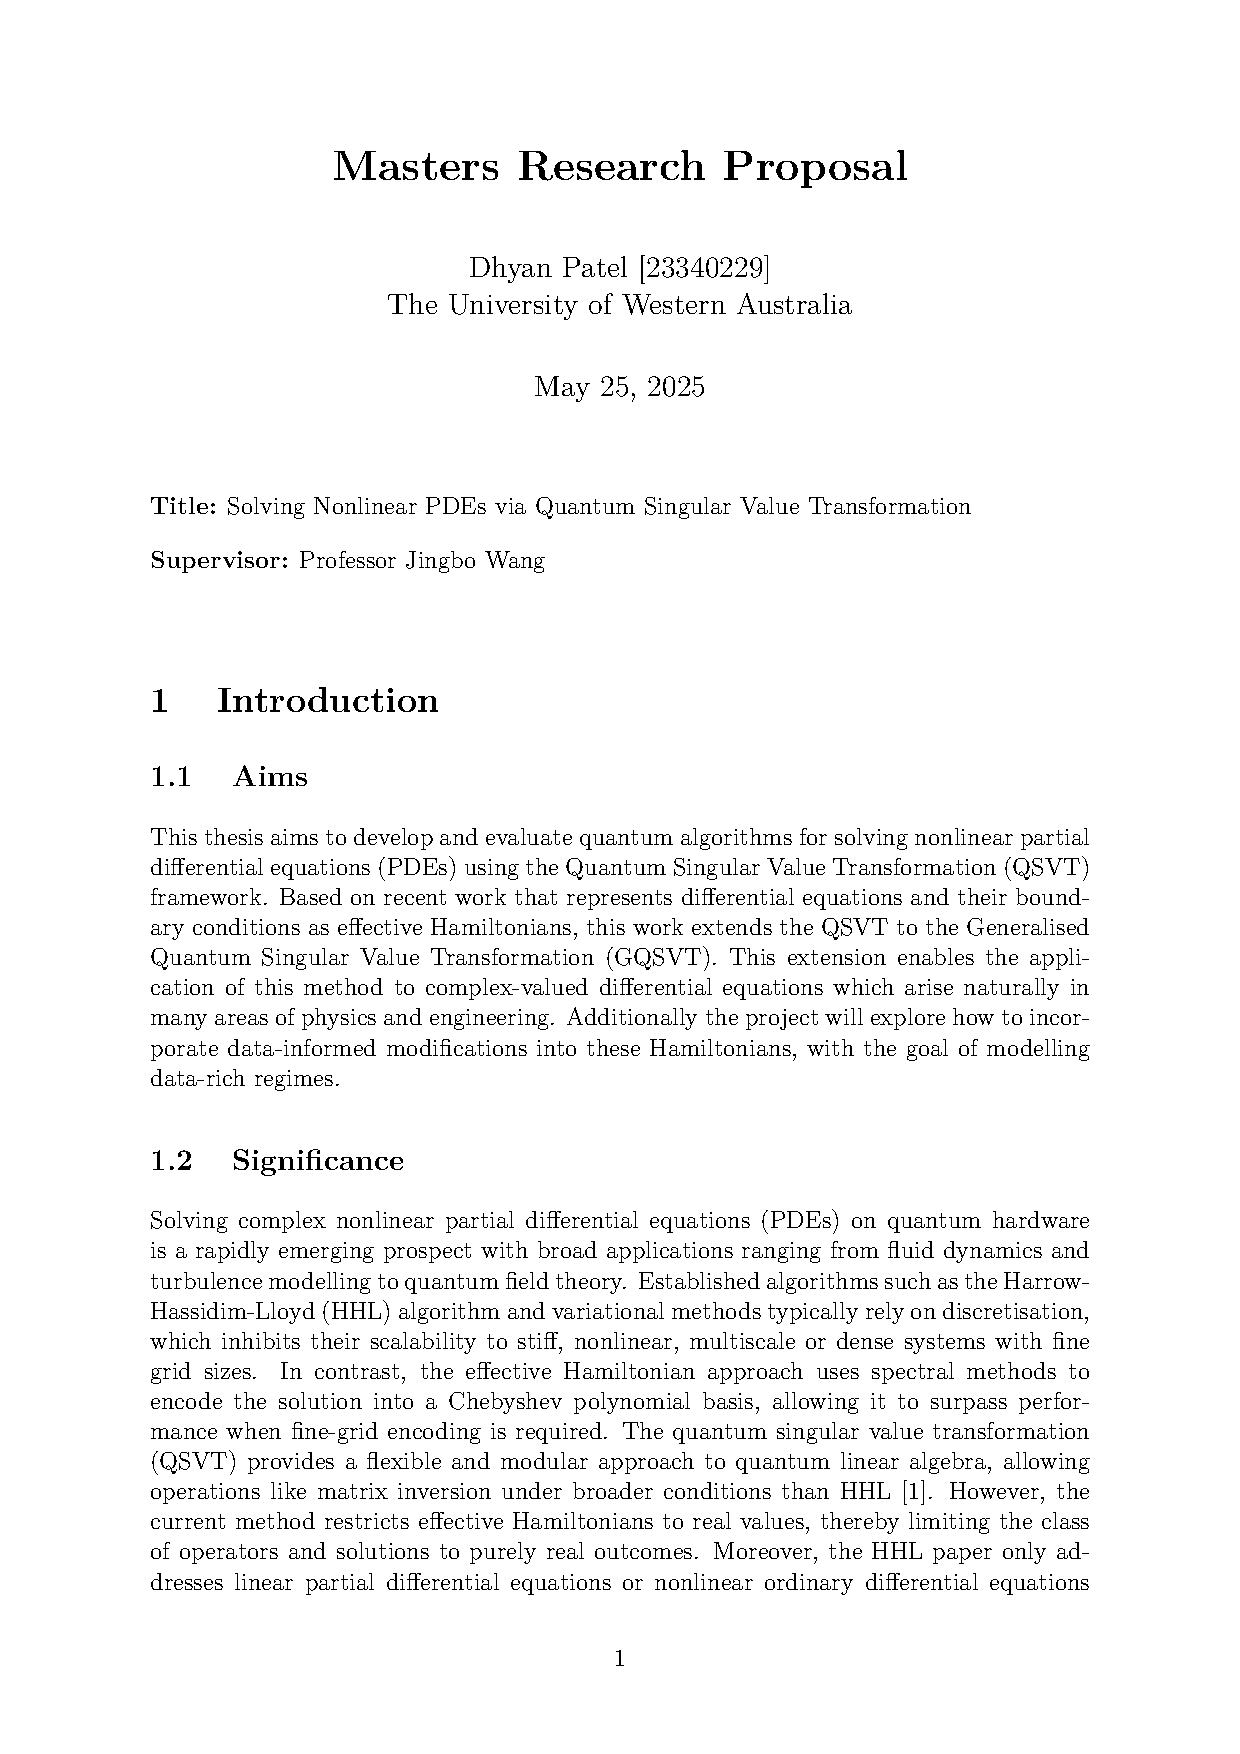
\includepdf[pages=-, scale=0.9, pagecommand={\thispagestyle{plain}}]{3_footer/research_proposal.pdf}

%
\endgroup

\end{document}
